\documentclass[b5paper, twosided]{book}
\usepackage{lipsum}
\usepackage[b5paper, width = 14.5cm, headheight = 2.0cm, tmargin=2.0cm, bmargin = 1.5cm, height=18.0cm, twoside, hmargin={1.5cm,1cm} ]{geometry}
\usepackage[english]{babel}
\usepackage{wallpaper}

\usepackage[square, sort&compress]{natbib}

\usepackage{amsmath, amssymb, amsfonts}
\usepackage{graphicx}
	\usepackage{makeidx}
\usepackage{nomencl}
\usepackage{multicol}
\usepackage{mathtools}
\usepackage{lettrine}



\usepackage{userManualStyle}
%\usepackage[latin2]{inputenc}


\usepackage{color}
\usepackage[unicode]{hyperref}
\hypersetup{
    colorlinks = true,%
    citecolor = [rgb]{0.0,0.0,0.75},
    filecolor=black,%	
    linkcolor = [rgb]{0.65,0.0,0.0},%
    anchorcolor = red,
    urlcolor= [rgb]{0.65,0.0,0.0}
}

\newcommand*{\citedelimiter}{; }
\makeatletter
\def\@citex[#1]#2{\leavevmode
  \let\@citea\@empty
  \@cite{\@for\@citeb:=#2\do
    {\@citea\def\@citea{\citedelimiter\penalty\@m}%
     \edef\@citeb{\expandafter\@firstofone\@citeb\@empty}%
     \if@filesw\immediate\write\@auxout{\string\citation{\@citeb}}\fi
     \@ifundefined{b@\@citeb}{\hbox{\reset@font\bfs	eries ?}%
       \G@refundefinedtrue
       \@latex@warning
         {Citation `\@citeb' on page \thepage \space undefined}}%
       {\@cite@ofmt{\csname b@\@citeb\endcsname}}}}{#1}}
\makeatother


\usepackage{listings}
\usepackage{color}
\usepackage{xcolor}
\usepackage{caption}
\usepackage{tikz}
\usepackage{mdframed}
\usepackage{transparent}

\DeclareCaptionFont{white}{\color{white}}

\definecolor{Teal}{rgb}{0.0, 0.4078431372549, 0.54296875}
\definecolor{TealBorder}{cmyk}{0.9, 0.0, 0.0, 0.0}
\definecolor{ListingBackgroundGray}{gray}{0.95}
\definecolor{ListingBorderGray}{gray}{0.75}

\newmdenv[tikzsetting={fill=ListingBackgroundGray,fill opacity=1.0, line width = 0, draw = ListingBackgroundGray}, backgroundcolor = none]{transparentbox}

\makeatletter
\lst@Key{countblanklines}{true}[t]%
{\lstKV@SetIf{#1}\lst@ifcountblanklines}

\lst@AddToHook{OnEmptyLine}{%
	\lst@ifnumberblanklines\else%
	\lst@ifcountblanklines\else%
	\advance\c@lstnumber-\@ne\relax%
	\fi%
	\fi}
\makeatother


\makeatletter
\AtBeginEnvironment{mdframed}{%
    \def\@fnsymbol#1{\ensuremath{\ifcase#1\or \dagger\or \ddagger\or
            \mathsection\or \mathparagraph\or \|\or **\or \dagger\dagger
            \or \ddagger\ddagger \or \copyright \else\@ctrerr\fi}}%
}   
\renewcommand\thempfootnote{\fnsymbol{mpfootnote}}
\makeatother


\let\origthelstnumber\thelstnumber

\makeatletter
\newcommand*\Suppressnumber{%
    \lst@AddToHook{OnNewLine}{%
        \let\thelstnumber\relax%
        \advance\c@lstnumber-\@ne\relax%
       }%
      }
      
\newcommand*\Reactivatenumber{%
  \lst@AddToHook{OnNewLine}{%
      \let\thelstnumber\origthelstnumber%
      \advance\c@lstnumber\@ne\relax}%
   }
   
   
\makeatother
           	
\newcommand{\ccode}[5]
{

	\lstset
	{
		%columns = fixed,%space-flexible,
		numberblanklines = false,
		countblanklines = false,
		escapeinside={(*@}{@*)},
		mathescape = true,
		showstringspaces=false,
%		backgroundcolor = \color[rgb]{0.95, 0.95, 0.95},
		firstnumber = {#1},	
		language = C++,
		classoffset = 0,
		morekeywords = {openmode, asin, size_t, floor, map, ios_base, undef, assert, min, rand, RAND_MAX, once, string, fstream, uniform, vec4, attribute, varying, vec3, max, normalize, gl_LightSource, gl_FrontMaterial, pow, version, gl_NormalMatrix, gl_Normal, gl_LightModel, ftransform, gl_Position, mat4, sampler2D,
        texture2DProj,
		gl_FragColor, gl_Vertex, gl_ModelViewMatrix, reflect, length, dot, clamp, gl_FrontLightModelProduct, gl_MaxLights, gl_BackMaterial, gl_BackLightModelProduct,
		gl_FragColor,
		istream, ostream, const_iterator, iterator, cos, sin, __FILE__, __LINE__,
		std, vector, memcpy, nothrow, define, pragma, omp, parallel, flush, critical, atomic, abs, nullptr, pair}, keywordstyle = {\color[rgb]{0.5, 0.0, 0.0}},
		classoffset = 1,
		morekeywords = {
        CARTESIANS3_H,
        HOMOGENEOUS3_H,
        COLORS4_H,
        TCOORDINATES4_H,
        GENERICCURVES3_H,
        LINEARCOMBINATIONS3_H,
        LIGHTS_H,
        MATERIALS_H,
        TENSORPRODUCTSURFACES3_H,
        TRIANGLEMESHES3_H,
        TRIANGULARFACES_H,
        CONSTANTS_H,
        GENERICGLTRANSFORMATIONS_H,
        MATRICES_H,
        PASCALTRIANGLES_H,
        REALMATRICES_H,
        REALMATRIXDECOMPOSITIONS_H,
        SPECIALGLTRANSFORMATIONS_H,
        SHADERPROGRAMS_H,
        CHECKINGPOLICIES_H,
        IMPLICITCONVERSIONPOLICIES_H,
        OWNERSHIPPOLICIES_H,
        SMARTPOINTERS_H,
        SPECIALIZEDSMARTPOINTERS_H,
        STATICCHECKS_H,
        STORAGEPOLICIES_H,
        TYPESELECTORS_H,
        EXCEPTIONS_H,
        UTILITIES_H,
        ABSTRACTBASES_H,
        CHARACTERISTICPOLYNOMIALS_H,
        ECSPACES_H,
        BCURVES3_H,
        BSURFACES3_H,
        YOURGLWIDGET_H,
        MACHINE_EPS,
        TINY,
        DEFAULT_NULL_FRAGMENT,
        X_VARIATION_FRAGMENT,
        Y_VARIATION_FRAGMENT,
        Z_VARIATION_FRAGMENT,
        NORMAL_LENGTH_FRAGMENT,
        GAUSSIAN_CURVATURE_FRAGMENT,
        MEAN_CURVATURE_FRAGMENT,
        WILLMORE_ENERGY_FRAGMENT,
        LOGARITHMIC_WILLMORE_ENERGY_FRAGMENT,
        UMBILIC_DEVIATION_ENERGY_FRAGMENT,
        LOGARITHMIC_UMBILIC_DEVIATION_ENERGY_FRAGMENT,
        TOTAL_CURVATURE_ENERGY_FRAGMENT,
        LOGARITHMIC_TOTAL_CURVATURE_ENERGY_FRAGMENT,
        LOG_WILLMORE_ENERGY_FRAGMENT,
        LOG_UMBILIC_DEVIATION_ENERGY_FRAGMENT,
        LOG_TOTAL_CURVATURE_ENERGY_FRAGMENT,
        ImageColorScheme,
        variable,
        colors, materials, toString, platformIsSupported, coldToHotColormap, openGLTypeToString,
        directionalLight,
        pointLight,
        spotlight,
        calculateAttenuation,
        calculateLighting,
        LightSource,
        RealMatrix,
        PLUDecomposition,
        FactorizedUnpivotedLUDecomposition,
        SVDecomposition,
        EuclideanNorm,
        sign,
        GLTransformation,
        MATRIX,
        SWAP_ROWS,
        Rotate,
        Scale,
        Translate,
        LookAt,
        OrthogonalProjection,
        PerspectiveProjection,
        VERTEX,
        FRAGMENT,
        COMPUTE,
        GEOMETRY,
        TESS_CONTROL,
        TESS_EVALUATION,
        ActiveVariable,
        Attribute, Uniform,
		CAGD, CalculateLighting,
		StoragePolicy, Default, Array, OwnershipPolicy, NoCopy, DeepCopy, DeepPrimitiveCopy, DestructiveCopy, ReferenceCounting, DESTRUCTIVE_COPY,
		CheckingPolicy, NoCheck, RejectNullDereferenceOrIndirection, RejectNull, AssertNullDereferenceOrIndirection, AssertNull, _CopiedType, _ImplicitConversionType,
		STATIC_CHECK, primitive, NullPointerException, 
		TypeSelector, Result, ImplicitConversionPolicy, Allowed, Disallowed, ENABLED, ImplicitConversionType, SmartPointer, NullPointerTester, CompileTimeError, Cartesian3, Homogeneous3,
		ONE_RADIAN, TWO_PI, Material, IsLightEnabled, CalculateAttenuation, AMBIENT_BLACK, DEFAULT_BLACK,
		Matrix, ColumnMatrix, RowMatrix, TriangularMatrix, RealSquareMatrix, Exception, HCoordinate, DirectionalLight, PointLight, Spotlight,
		GenericCurve, ShaderProgram, Shader,
		SmoothParametricCurve,
		ptrVectorValuedFunction1V,
		ptrVectorValuedFunction2V,
		SplineInformation,
		ApproximatingSpline,ColdToHotColormap,
		SomeApproximatingCurve,
		Vertex, Face, Color, TextureCoordinate, TriangularFace, TCoordinate, TriangulatedMesh, AbstractTensorProductSurface, SurfaceInformation, BicubicBezierPatch,
		EPS, cagd, GLWidget, GenericCurve3, YourGLWidget,Derivatives,
		ECSpace, CharacteristicPolynomial, DefaultPrimitive, NonIntrusiveReferenceCounting, BasisFunctionType, ORDINARY_BASIS, LinearCombination3, PolynomialECSpace, TrigonometricECSpace, HyperbolicECSpace, NON_NEGATIVE_NORMALIZED_B_BASIS, SP, PI, Default, Zero, _OrdinaryBasisFunction, Type, AET_COSINE, AET_SINE, AE_COSINE, AE_SINE, AT_COSINE, AT_SINE, P_COSINE, P_SINE, HyperbolicBCurve3, BCurve3, AbstractBase, _Disallowed, TensorProductSurface3, TriangleMesh3, TCoordinate4, PartialDerivatives, DirectionalDerivatives, VARIABLE, B_BASIS, BC, BSurface3, OrdinarySurfaceCoefficients, PascalTriangle, Color4, HALF_PI, DEG_TO_RADIAN, BC_SIZE, MAX_DIFF_ORDER, ATECSpace, AETECSpace, SnailUECSpace, SnailVECSpace, BrilleaudMazureSpace, Renderable}, 
		keywordstyle = {\color[rgb]{0.0, 0.0, 0.70}},
		classoffset = 2,
		morekeywords = {
            glClearColor,
            GL_DEPTH_TEST,
        glGetIntegerv, 
        glGetAttachedShaders,
        GL_CURRENT_PROGRAM,
        GL_ACTIVE_ATTRIBUTES,
        GL_ACTIVE_ATTRIBUTE_MAX_LENGTH,
        glGetActiveAttrib,
        GL_FLOAT_VEC3,
        GL_FLOAT_VEC4,
        GL_FLOAT_VEC2,
        GL_INT,
        GL_INT_VEC2,
        GL_INT_VEC3,
        GL_INT_VEC4,
        GL_UNSIGNED_INT_VEC2,
        GL_UNSIGNED_INT_VEC3,
        GL_UNSIGNED_INT_VEC4,
        GL_BOOL,
        GL_BOOL_VEC2,
        GL_BOOL_VEC3,
        GL_BOOL_VEC4,
        GL_FLOAT_MAT2,
        GL_FLOAT_MAT3,
        GL_FLOAT_MAT4,
        GL_FLOAT_MAT2x3,
        GL_FLOAT_MAT2x4,
        GL_FLOAT_MAT3x2,
        GL_FLOAT_MAT3x4,
        GL_FLOAT_MAT4x2,
        GL_FLOAT_MAT4x3,
        GL_SAMPLER_1D,
        GL_SAMPLER_2D,
        GL_SAMPLER_3D,
        GL_SAMPLER_CUBE,
        GL_SAMPLER_1D_SHADOW,
        GL_SAMPLER_2D_SHADOW,
        GL_SAMPLER_1D_ARRAY,
        GL_SAMPLER_2D_ARRAY,
        GL_SAMPLER_1D_ARRAY_SHADOW,
        GL_SAMPLER_2D_ARRAY_SHADOW,
        GL_SAMPLER_2D_MULTISAMPLE,
        GL_SAMPLER_2D_MULTISAMPLE_ARRAY,
        GL_SAMPLER_CUBE_SHADOW,
        GL_SAMPLER_BUFFER,
        GL_SAMPLER_2D_RECT,
        GL_SAMPLER_2D_RECT_SHADOW,
        GL_INT_SAMPLER_1D,
        GL_INT_SAMPLER_2D,
        GL_INT_SAMPLER_3D,
        GL_INT_SAMPLER_CUBE,
        GL_INT_SAMPLER_1D_ARRAY,
        GL_INT_SAMPLER_2D_ARRAY,
        GL_INT_SAMPLER_2D_MULTISAMPLE,
        GL_INT_SAMPLER_2D_MULTISAMPLE_ARRAY,
        GL_INT_SAMPLER_BUFFER,
        GL_INT_SAMPLER_2D_RECT,
        GL_UNSIGNED_INT_SAMPLER_1D,
        GL_UNSIGNED_INT_SAMPLER_2D,
        GL_UNSIGNED_INT_SAMPLER_3D,
        GL_UNSIGNED_INT_SAMPLER_CUBE,
        GL_UNSIGNED_INT_SAMPLER_1D_ARRAY,
        GL_UNSIGNED_INT_SAMPLER_2D_ARRAY,
        GL_UNSIGNED_INT_SAMPLER_2D_MULTISAMPLE,
        GL_UNSIGNED_INT_SAMPLER_2D_MULTISAMPLE_ARRAY,
        GL_UNSIGNED_INT_SAMPLER_BUFFER,
        GL_UNSIGNED_INT_SAMPLER_2D_RECT,
        GLsizeiptr,
        T, ET, U, V, TSP, TOP, TICP, TCP, USP, UOP, UICP, UCP, VSP, VOP, VICP, VCP, glPointSize, glLineWidth, glTranslatef,
		GL_POINTS, GL_LINES, GL_POLYGON_OFFSET_FILL, glPolygonOffset, GL_LINE_SMOOTH, GL_LINE_SMOOTH_HINT, GL_POINT_SMOOTH, GL_POINT_SMOOTH_HINT, GL_NICEST, glHint, GLEW_OK, GL_LINE_STRIP, GL_LINE_LOOP, GL_TRIANGLES, GL_TRIANGLE_STRIP, GL_TRIANGLE_FAN, GL_QUADS, GL_QUAD_STRIP, GL_POLYGON,
		GL_STATIC_DRAW, GL_STATIC_READ, GL_STATIC_COPY,
		GL_STREAM_DRAW, GL_STREAM_READ, GL_STREAM_COPY,
		GL_DYNAMIC_DRAW, GL_DYNAMIC_READ, GL_DYNAMIC_COPY,
		GL_VERTEX_ARRAY, GL_ARRAY_BUFFER, GL_FLOAT, GL_DOUBLE,
		GL_LIGHT0, GL_LIGHT1, GL_LIGHT2, GL_LIGHT3, GL_LIGHT4, GL_LIGHT5, GL_LIGHT6, GL_LIGHT7, 
		GL_POSITION, GL_SPOT_CUTOFF, GL_SPOT_EXPONENT, GL_CONSTANT_ATTENUATION, GL_LINE_STIPPLE, glLineStipple, GL_LINEAR_ATTENUATION, GL_QUADRATIC_ATTENUATION, GL_SPOT_DIRECTION,
		GL_BLEND, GL_TRUE, GL_FALSE, GL_DEPTH, GLUT_DOUBLE, GLUT_DEPTH, GLUT_RGBA, GL_SRC_ALPHA, GL_ONE_MINUS_SRC_ALPHA, GL_ONE, GL_WRITE_ONLY, GL_READ_ONLY, GL_READ_WRITE,
		GL_LIGHTING, GL_NORMALIZE,
		glClear,
		GL_COLOR_BUFFER_BIT, GL_DEPTH_BUFFER_BIT,
		glPushMatrix, glPopMatrix,
		GLint, GLuint,
		GLboolean,glMapBuffer, glUnmapBuffer,glMaterial,glMaterialf, glMaterialfv,GL_FRONT, GL_BACK, GL_FRONT_AND_BACK, GL_AMBIENT, GL_SPECULAR, GL_DIFFUSE, GL_EMISSION, GL_SHININESS,
		GLfloat, GLdouble, glDrawElements,glTexCoordPointer, glNormalPointer, glVertexPointer, GL_ELEMENT_ARRAY_BUFFER, GL_NORMAL_ARRAY, GL_TEXTURE_COORD_ARRAY,GL_UNSIGNED_INT,
        GL_NONE,
        GL_COMPUTE_SHADER,
        GL_GEOMETRY_SHADER,
        GL_TESS_CONTROL_SHADER,
        GL_TESS_EVALUATION_SHADER,
        GL_ATTACHED_SHADERS,
        GL_ACTIVE_UNIFORMS,
        GL_ACTIVE_UNIFORM_MAX_LENGTH,
        glGetActiveUniform,
        glGetUniformLocation,
        GL_ACTIVE_ATTRIBUTES,
        GL_ACTIVE_ATTRIBUTE_MAX_LENGTH,
        glUniform1ui,
        glUniform2ui,
        glUniform3ui,
        glUniform4ui,
        glUniform1uiv,
        glUniform2uiv,
        glUniform3uiv,
        glUniform4uiv,
        glUniformMatrix4x3fv,
		GLenum,
		GLvoid, GL_DST_ALPHA, GL_ONE_MINUS_DST_ALPHA, glCullFace, GL_CULL_FACE, 
		glBegin, glEnd, GLushort,
		glUnmapBuffer, glGenBuffers, glBindBuffer, glBufferData, glVertexPointer, glDrawArrays, glEnableClientState, glDisableClientState, glDeleteBuffers,
		glVertex3f, glVertex3fv, glNormal3f, glNormal3fv, glScalef, glTranslate, glRotate, glMultMatrixf, glGenLists, glDeleteLists, glEnable, glDisable,
		glColor3f, glColor3fv, glColor4f, glColor4fv,
		glNormal3f, glNormal3fv,
		glTexCoord2f, glTexCoord2fv, glDepthMask, glBlendFunc, glewInit, glewIsSupported, GLEW_ARB_vertex_shader, GLEW_ARB_fragment_shader,
		glCreateShader, glShaderSource, glCompileShader, glCreateProgram, glAttachShader, glLinkProgram, glUseProgram, GLsizei, GLchar, glValidateProgram, glDetachShader, glDeleteShader,
		glGetShaderInfoLog, glGetShaderiv, glGetProgramInfoLog, glGetProgramiv, glDeleteProgram, GL_VERTEX_SHADER, GL_FRAGMENT_SHADER, GL_COMPILE_STATUS, GL_LINK_STATUS, GL_NO_ERROR, glGetError,
		gluErrorString, GL_VALIDATE_STATUS, GL_INFO_LOG_LENGTH, GetUniformVariableLocation, glUniform1f, glUniform2f, glUniform3f, 
		glUniform1i, glUniform4f, glUniform2i, glUniform3i, glUniform4i,
		glUniform1fv, glUniform2fv, glUniform3fv, glUniform4fv,
		glUniform1iv, glUniform2iv, glUniform3iv, glUniform4iv,
		glUniformMatrix2fv, glUniformMatrix3fv, glUniformMatrix4fv, glUniformMatrix2x3fv, glUniformMatrix3x2fv, glUniformMatrix2x4fv, glUniformMatrix4x2fv, glUniformMatrix3x4fv, glUniformMatrix4x3fv
		GLushort, GLubyte, GLshort, GLbyte,
		glVertexAttrib1f, glVertexAttrib1s, glVertexAttrib1d,
		glVertexAttrib2f, glVertexAttrib2s, glVertexAttrib2d,
		glVertexAttrib3f, glVertexAttrib3s, glVertexAttrib3d,
		glVertexAttrib4f, glVertexAttrib4s, glVertexAttrib4d, glVertexAttrib4Nub,
		glVertexAttrib1fv, glVertexAttrib1sv, glVertexAttrib1dv,
		glVertexAttrib2fv, glVertexAttrib2sv, glVertexAttrib2dv,
		glVertexAttrib3fv, glVertexAttrib3sv, glVertexAttrib3dv,
		glVertexAttrib4fv, glVertexAttrib4sv, glVertexAttrib4dv, glVertexAttrib4Nubv,
		glVertexAttrib4ubv, glVertexAttrib4usv, glVertexAttrib4uiv, glVertexAttrib4Nbv, glVertexAttrib4Nsv, glVertexAttrib4Niv, glVertexAttrib4Nuiv, glVertexAttrib4Nusv, glVertexAttrib4Nubv,
		glVertexAttrib4iv, glVertexAttrib4bv, glGetAttribLocation, glVertexAttribPointer, glEnableVertexAttribArray, glDisableVertexAttribArray
		}, keywordstyle = {\color[rgb]{1.0, 0.0, 0.6}},
		classoffset = 3,
		morekeywords = {in, out, app, inout}, keywordstyle = {\color[rgb]{1.0, 0.0, 0.0}},
		classoffset = 0,
		commentstyle = {\color[rgb]{0.0, 0.5, 0.0}},
		basicstyle = \linespread{1}\scriptsize,
		numbers = left, numberstyle = \tiny, numbersep = 5 pt
	}
	
	\refstepcounter{lstlisting}\label{#3}
	\vspace{0.5\baselineskip}
%	\setlength{\fboxrule}{0.25pt}
	\noindent{}\fcolorbox{black}{Teal}{\parbox{0.985\textwidth}{\footnotesize{\White{\textbf{Listing \thelstlisting.} #4}}}}
%	\vspace{-1.25\baselineskip}
	\begin{mdframed}[backgroundcolor = ListingBackgroundGray, linecolor = ListingBorderGray, linewidth = 0.25pt, skipabove = -0.5pt, skipbelow = 0.33\baselineskip, innertopmargin = 0pt, innerbottommargin = 0pt, innerleftmargin = 0pt, innerrightmargin = 0pt]
%	\lstinputlisting[label = #3, caption = #4]{#2}
%	\lstinputlisting[label = #3]{#2}
	\lstinputlisting[firstline = {#5}]{#2}
%    \addcontentsline{CODE}{ccode}
%    {\protect\numberline{\thelstlisting}#4}\par
	\end{mdframed}
}

\newcommand{\ccodeNUV}[5]
{
	
	\lstset
	{
		%columns = fixed,%space-flexible,
		numberblanklines = false,
		countblanklines = false,
		escapeinside={(*@}{@*)},
		mathescape = true,
		showstringspaces=false,
		%		backgroundcolor = \color[rgb]{0.95, 0.95, 0.95},
		firstnumber = {#1},	
		language = C++,
		classoffset = 0,
		morekeywords = {openmode, asin, size_t, floor, map, ios_base, undef, assert, min, rand, RAND_MAX, once, string, fstream, uniform, vec4, attribute, varying, vec3, max, normalize, gl_LightSource, gl_FrontMaterial, pow, gl_NormalMatrix, gl_Normal, gl_LightModel, ftransform, gl_Position, mat4, sampler2D, 
            texture2DProj,
            version,
			gl_FragColor, gl_Vertex, gl_ModelViewMatrix, reflect, length, dot, clamp, gl_FrontLightModelProduct, gl_MaxLights, gl_BackMaterial, gl_BackLightModelProduct,
			gl_FragColor,
			istream, ostream, const_iterator, iterator, cos, sin, __FILE__, __LINE__,
			std, vector, memcpy, nothrow, define, pragma, omp, parallel, flush, critical, atomic, abs, nullptr, pair}, keywordstyle = {\color[rgb]{0.5, 0.0, 0.0}},
		classoffset = 1,
		morekeywords = {
            CARTESIANS3_H,
            HOMOGENEOUS3_H,
            COLORS4_H,
            TCOORDINATES4_H,
            GENERICCURVES3_H,
            LINEARCOMBINATIONS3_H,
            LIGHTS_H,
            MATERIALS_H,
            TENSORPRODUCTSURFACES3_H,
            TRIANGLEMESHES3_H,
            TRIANGULARFACES_H,
            CONSTANTS_H,
            GENERICGLTRANSFORMATIONS_H,
            MATRICES_H,
            PASCALTRIANGLES_H,
            REALMATRICES_H,
            REALMATRIXDECOMPOSITIONS_H,
            SPECIALGLTRANSFORMATIONS_H,
            SHADERPROGRAMS_H,
            CHECKINGPOLICIES_H,
            IMPLICITCONVERSIONPOLICIES_H,
            OWNERSHIPPOLICIES_H,
            SMARTPOINTERS_H,
            SPECIALIZEDSMARTPOINTERS_H,
            STATICCHECKS_H,
            STORAGEPOLICIES_H,
            TYPESELECTORS_H,
            EXCEPTIONS_H,
            UTILITIES_H,
            ABSTRACTBASES_H,
            CHARACTERISTICPOLYNOMIALS_H,
            ECSPACES_H,
            BCURVES3_H,
            BSURFACES3_H,
            YOURGLWIDGET_H,
            MACHINE_EPS,
            TINY,
            DEFAULT_NULL_FRAGMENT,
            X_VARIATION_FRAGMENT,
            Y_VARIATION_FRAGMENT,
            Z_VARIATION_FRAGMENT,
            NORMAL_LENGTH_FRAGMENT,
            GAUSSIAN_CURVATURE_FRAGMENT,
            MEAN_CURVATURE_FRAGMENT,
            WILLMORE_ENERGY_FRAGMENT,
            LOGARITHMIC_WILLMORE_ENERGY_FRAGMENT,
            UMBILIC_DEVIATION_ENERGY_FRAGMENT,
            LOGARITHMIC_UMBILIC_DEVIATION_ENERGY_FRAGMENT,
            TOTAL_CURVATURE_ENERGY_FRAGMENT,
            LOGARITHMIC_TOTAL_CURVATURE_ENERGY_FRAGMENT,
            LOG_WILLMORE_ENERGY_FRAGMENT,
            LOG_UMBILIC_DEVIATION_ENERGY_FRAGMENT,
            LOG_TOTAL_CURVATURE_ENERGY_FRAGMENT,
            ImageColorScheme,
            variable,
            colors, materials, toString, platformIsSupported, coldToHotColormap, openGLTypeToString,
            directionalLight,
            pointLight,
            spotlight,
            calculateAttenuation,
            calculateLighting,
            LightSource,
            RealMatrix,
            PLUDecomposition,
            FactorizedUnpivotedLUDecomposition,
            SVDecomposition,
            EuclideanNorm,
            sign,
            GLTransformation,
            MATRIX,
            SWAP_ROWS,
            Rotate,
            Scale,
            Translate,
            LookAt,
            OrthogonalProjection,
            PerspectiveProjection,
            VERTEX,
            FRAGMENT,
            COMPUTE,
            GEOMETRY,
            TESS_CONTROL,
            TESS_EVALUATION,
            ActiveVariable,
            Attribute, Uniform,
            ColdToHotColormap,
			CAGD, CalculateLighting,
			StoragePolicy, Default, Array, OwnershipPolicy, NoCopy, DeepCopy, DeepPrimitiveCopy, DestructiveCopy, ReferenceCounting, DESTRUCTIVE_COPY,
			CheckingPolicy, NoCheck, RejectNullDereferenceOrIndirection, RejectNull, AssertNullDereferenceOrIndirection, AssertNull, _CopiedType, _ImplicitConversionType,
			STATIC_CHECK, primitive, NullPointerException, 
			TypeSelector, Result, ImplicitConversionPolicy, Allowed, Disallowed, ENABLED, ImplicitConversionType, SmartPointer, NullPointerTester, CompileTimeError, Cartesian3, Homogeneous3,
			ONE_RADIAN, TWO_PI, Material, IsLightEnabled, CalculateAttenuation, AMBIENT_BLACK, DEFAULT_BLACK,
			Matrix, ColumnMatrix, RowMatrix, TriangularMatrix, RealSquareMatrix, Exception, HCoordinate, DirectionalLight, PointLight, Spotlight,
			GenericCurve, ShaderProgram, Shader,
			SmoothParametricCurve,
			ptrVectorValuedFunction1V,
			ptrVectorValuedFunction2V,
			SplineInformation,
			ApproximatingSpline,
			SomeApproximatingCurve,
			Vertex, Face, Color, TextureCoordinate, TriangularFace, TCoordinate, TriangulatedMesh, AbstractTensorProductSurface, SurfaceInformation, BicubicBezierPatch,
			EPS, cagd, GLWidget, GenericCurve3, YourGLWidget,Derivatives,
			ECSpace, CharacteristicPolynomial, DefaultPrimitive, NonIntrusiveReferenceCounting, BasisFunctionType, ORDINARY_BASIS, LinearCombination3, PolynomialECSpace, TrigonometricECSpace, HyperbolicECSpace, NON_NEGATIVE_NORMALIZED_B_BASIS, SP, PI, Default, Zero, _OrdinaryBasisFunction, Type, AET_COSINE, AET_SINE, AE_COSINE, AE_SINE, AT_COSINE, AT_SINE, P_COSINE, P_SINE, HyperbolicBCurve3, BCurve3, AbstractBase, _Disallowed, TensorProductSurface3, TriangleMesh3, TCoordinate4, PartialDerivatives, DirectionalDerivatives, U, V, VARIABLE, B_BASIS, BC, BSurface3, OrdinarySurfaceCoefficients, PascalTriangle, Color4, HALF_PI, DEG_TO_RADIAN, BC_SIZE, MAX_DIFF_ORDER, ATECSpace, AETECSpace, SnailUECSpace, SnailVECSpace, BrilleaudMazureSpace, Renderable}, 
		keywordstyle = {\color[rgb]{0.0, 0.0, 0.70}},
		classoffset = 2,
		morekeywords = {
            glClearColor,
            GL_DEPTH_TEST,
            glGetIntegerv, 
            GL_CURRENT_PROGRAM,
            GL_ACTIVE_ATTRIBUTES,
            GL_ACTIVE_ATTRIBUTE_MAX_LENGTH,
            glGetActiveAttrib,
            GL_FLOAT_VEC3,
            GL_FLOAT_VEC4,
            GL_FLOAT_VEC2,
            GL_INT,
            GL_INT_VEC2,
            GL_INT_VEC3,
            GL_INT_VEC4,
            GL_UNSIGNED_INT_VEC2,
            GL_UNSIGNED_INT_VEC3,
            GL_UNSIGNED_INT_VEC4,
            GL_BOOL,
            GL_BOOL_VEC2,
            GL_BOOL_VEC3,
            GL_BOOL_VEC4,
            GL_FLOAT_MAT2,
            GL_FLOAT_MAT3,
            GL_FLOAT_MAT4,
            GL_FLOAT_MAT2x3,
            GL_FLOAT_MAT2x4,
            GL_FLOAT_MAT3x2,
            GL_FLOAT_MAT3x4,
            GL_FLOAT_MAT4x2,
            GL_FLOAT_MAT4x3,
            GL_SAMPLER_1D,
            GL_SAMPLER_2D,
            GL_SAMPLER_3D,
            GL_SAMPLER_CUBE,
            GL_SAMPLER_1D_SHADOW,
            GL_SAMPLER_2D_SHADOW,
            GL_SAMPLER_1D_ARRAY,
            GL_SAMPLER_2D_ARRAY,
            GL_SAMPLER_1D_ARRAY_SHADOW,
            GL_SAMPLER_2D_ARRAY_SHADOW,
            GL_SAMPLER_2D_MULTISAMPLE,
            GL_SAMPLER_2D_MULTISAMPLE_ARRAY,
            GL_SAMPLER_CUBE_SHADOW,
            GL_SAMPLER_BUFFER,
            GL_SAMPLER_2D_RECT,
            GL_SAMPLER_2D_RECT_SHADOW,
            GL_INT_SAMPLER_1D,
            GL_INT_SAMPLER_2D,
            GL_INT_SAMPLER_3D,
            GL_INT_SAMPLER_CUBE,
            GL_INT_SAMPLER_1D_ARRAY,
            GL_INT_SAMPLER_2D_ARRAY,
            GL_INT_SAMPLER_2D_MULTISAMPLE,
            GL_INT_SAMPLER_2D_MULTISAMPLE_ARRAY,
            GL_INT_SAMPLER_BUFFER,
            GL_INT_SAMPLER_2D_RECT,
            GL_UNSIGNED_INT_SAMPLER_1D,
            GL_UNSIGNED_INT_SAMPLER_2D,
            GL_UNSIGNED_INT_SAMPLER_3D,
            GL_UNSIGNED_INT_SAMPLER_CUBE,
            GL_UNSIGNED_INT_SAMPLER_1D_ARRAY,
            GL_UNSIGNED_INT_SAMPLER_2D_ARRAY,
            GL_UNSIGNED_INT_SAMPLER_2D_MULTISAMPLE,
            GL_UNSIGNED_INT_SAMPLER_2D_MULTISAMPLE_ARRAY,
            GL_UNSIGNED_INT_SAMPLER_BUFFER,
            GL_UNSIGNED_INT_SAMPLER_2D_RECT,
            GLsizeiptr,
            TSP, TOP, TICP, TCP, USP, UOP, UICP, UCP, VSP, VOP, VICP, VCP, glPointSize,
			GL_POINTS, GL_LINES, GL_POLYGON_OFFSET_FILL, glPolygonOffset, GL_LINE_SMOOTH, GL_LINE_SMOOTH_HINT, GL_POINT_SMOOTH, GL_POINT_SMOOTH_HINT, GL_NICEST, glHint, GLEW_OK, GL_LINE_STRIP, GL_LINE_LOOP, GL_TRIANGLES, GL_TRIANGLE_STRIP, GL_TRIANGLE_FAN, GL_QUADS, GL_QUAD_STRIP, GL_POLYGON,
			GL_STATIC_DRAW, GL_STATIC_READ, GL_STATIC_COPY,
			GL_STREAM_DRAW, GL_STREAM_READ, GL_STREAM_COPY,
			GL_DYNAMIC_DRAW, GL_DYNAMIC_READ, GL_DYNAMIC_COPY,
			GL_VERTEX_ARRAY, GL_ARRAY_BUFFER, GL_FLOAT, GL_DOUBLE,GL_LINE_STIPPLE, glLineStipple,
			GL_LIGHT0, GL_LIGHT1, GL_LIGHT2, GL_LIGHT3, GL_LIGHT4, GL_LIGHT5, GL_LIGHT6, GL_LIGHT7, 
			GL_POSITION, GL_SPOT_CUTOFF, GL_SPOT_EXPONENT, GL_CONSTANT_ATTENUATION, GL_LINEAR_ATTENUATION, GL_QUADRATIC_ATTENUATION, GL_SPOT_DIRECTION,
			GL_BLEND, GL_TRUE, GL_FALSE, GL_DEPTH, GLUT_DOUBLE, GLUT_DEPTH, GLUT_RGBA, GL_SRC_ALPHA, GL_ONE_MINUS_SRC_ALPHA, GL_ONE, GL_WRITE_ONLY, GL_READ_ONLY, GL_READ_WRITE,
			GL_LIGHTING, GL_NORMALIZE,
			glClear,
			GL_COLOR_BUFFER_BIT, GL_DEPTH_BUFFER_BIT,
			glPushMatrix, glPopMatrix, glGetAttachedShaders,
			GLint, GLuint,
			GLboolean,glMapBuffer, glUnmapBuffer,glMaterial,glMaterialf, glMaterialfv,GL_FRONT, GL_BACK, GL_FRONT_AND_BACK, GL_AMBIENT, GL_SPECULAR, GL_DIFFUSE, GL_EMISSION, GL_SHININESS,
			GLfloat, GLdouble, glDrawElements,glTexCoordPointer, glNormalPointer, glVertexPointer, GL_ELEMENT_ARRAY_BUFFER, GL_NORMAL_ARRAY, GL_TEXTURE_COORD_ARRAY,GL_UNSIGNED_INT,
            GL_NONE,
            GL_COMPUTE_SHADER,
            GL_GEOMETRY_SHADER,
            GL_TESS_CONTROL_SHADER,
            GL_TESS_EVALUATION_SHADER,
            GL_ATTACHED_SHADERS,
            GL_ACTIVE_UNIFORMS,
            GL_ACTIVE_UNIFORM_MAX_LENGTH,
            glGetActiveUniform,
            glGetUniformLocation,
            GL_ACTIVE_ATTRIBUTES,
            GL_ACTIVE_ATTRIBUTE_MAX_LENGTH,
            glUniform1ui,
            glUniform2ui,
            glUniform3ui,
            glUniform4ui,
            glUniform1uiv,
            glUniform2uiv,
            glUniform3uiv,
            glUniform4uiv,
            glUniformMatrix4x3fv,
			GLenum,
			GLvoid, GL_DST_ALPHA, GL_ONE_MINUS_DST_ALPHA, glCullFace, GL_CULL_FACE, glLineWidth, glTranslatef,
			glBegin, glEnd, GLushort,
			glUnmapBuffer, glGenBuffers, glBindBuffer, glBufferData, glVertexPointer, glDrawArrays, glEnableClientState, glDisableClientState, glDeleteBuffers,
			glVertex3f, glVertex3fv, glNormal3f, glNormal3fv, glScalef, glTranslate, glRotate, glMultMatrixf, glGenLists, glDeleteLists, glEnable, glDisable,
			glColor3f, glColor3fv, glColor4f, glColor4fv,
			glNormal3f, glNormal3fv,
			glTexCoord2f, glTexCoord2fv, glDepthMask, glBlendFunc, glewInit, glewIsSupported, GLEW_ARB_vertex_shader, GLEW_ARB_fragment_shader,
			glCreateShader, glShaderSource, glCompileShader, glCreateProgram, glAttachShader, glLinkProgram, glUseProgram, GLsizei, GLchar, glValidateProgram, glDetachShader, glDeleteShader,
			glGetShaderInfoLog, glGetShaderiv, glGetProgramInfoLog, glGetProgramiv, glDeleteProgram, GL_VERTEX_SHADER, GL_FRAGMENT_SHADER, GL_COMPILE_STATUS, GL_LINK_STATUS, GL_NO_ERROR, glGetError,
			gluErrorString, GL_VALIDATE_STATUS, GL_INFO_LOG_LENGTH, GetUniformVariableLocation, glUniform1f, glUniform2f, glUniform3f, 
			glUniform1i, glUniform4f, glUniform2i, glUniform3i, glUniform4i,
			glUniform1fv, glUniform2fv, glUniform3fv, glUniform4fv,
			glUniform1iv, glUniform2iv, glUniform3iv, glUniform4iv,
			glUniformMatrix2fv, glUniformMatrix3fv, glUniformMatrix4fv, glUniformMatrix2x3fv, glUniformMatrix3x2fv, glUniformMatrix2x4fv, glUniformMatrix4x2fv, glUniformMatrix3x4fv, glUniformMatrix4x3fv
			GLushort, GLubyte, GLshort, GLbyte,
			glVertexAttrib1f, glVertexAttrib1s, glVertexAttrib1d,
			glVertexAttrib2f, glVertexAttrib2s, glVertexAttrib2d,
			glVertexAttrib3f, glVertexAttrib3s, glVertexAttrib3d,
			glVertexAttrib4f, glVertexAttrib4s, glVertexAttrib4d, glVertexAttrib4Nub,
			glVertexAttrib1fv, glVertexAttrib1sv, glVertexAttrib1dv,
			glVertexAttrib2fv, glVertexAttrib2sv, glVertexAttrib2dv,
			glVertexAttrib3fv, glVertexAttrib3sv, glVertexAttrib3dv,
			glVertexAttrib4fv, glVertexAttrib4sv, glVertexAttrib4dv, glVertexAttrib4Nubv,
			glVertexAttrib4ubv, glVertexAttrib4usv, glVertexAttrib4uiv, glVertexAttrib4Nbv, glVertexAttrib4Nsv, glVertexAttrib4Niv, glVertexAttrib4Nuiv, glVertexAttrib4Nusv, glVertexAttrib4Nubv,
			glVertexAttrib4iv, glVertexAttrib4bv, glGetAttribLocation, glVertexAttribPointer, glEnableVertexAttribArray, glDisableVertexAttribArray
		}, keywordstyle = {\color[rgb]{1.0, 0.0, 0.6}},
		classoffset = 3,
		morekeywords = {in, out,app, inout}, keywordstyle = {\color[rgb]{1.0, 0.0, 0.0}},
		classoffset = 0,
		commentstyle = {\color[rgb]{0.0, 0.5, 0.0}},
		basicstyle = \linespread{1}\scriptsize,
		numbers = left, numberstyle = \tiny, numbersep = 5 pt
	}
	
	\refstepcounter{lstlisting}\label{#3}
	\vspace{0.5\baselineskip}
	%	\setlength{\fboxrule}{0.25pt}
	\noindent{}\fcolorbox{black}{Teal}{\parbox{0.985\textwidth}{\footnotesize{\White{\textbf{Listing \thelstlisting.} #4}}}}
	%	\vspace{-1.25\baselineskip}
	\begin{mdframed}[backgroundcolor = ListingBackgroundGray, linecolor = ListingBorderGray, linewidth = 0.25pt, skipabove = -0.5pt, skipbelow = 0.33\baselineskip, innertopmargin = 0pt, innerbottommargin = 0pt, innerleftmargin = 0pt, innerrightmargin = 0pt]
		%	\lstinputlisting[label = #3, caption = #4]{#2}
		%	\lstinputlisting[label = #3]{#2}
		\lstinputlisting[firstline = {#5}]{#2}
%    \addcontentsline{CODE}{ccode}
%    {\protect\numberline{\thelstlisting}#4}\par
	\end{mdframed}
}


\newcommand{\ccodenonumber}[1]
{

	\lstset
	{
		escapeinside={(*@}{@*)},
		backgroundcolor = \color[rgb]{0.95, 0.95, 0.95},
		showstringspaces=false,
		language = C++,
		classoffset = 0,
		morekeywords = {openmode, asin, size_t, floor, map,ios_base, undef,RAND_MAX, rand, string, fstream, uniform, vec4, attribute, varying, vec3, max, nothrow, normalize, gl_LightSource, gl_FrontMaterial, pow, gl_NormalMatrix, gl_Normal, gl_LightModel, ftransform, gl_Position,
		gl_Vertex, gl_ModelViewMatrix,
		istream, ostream, version, const_iterator, iterator, cos, sin, __FILE__, __LINE__,
		std, vector,memcpy, vec, bvec, ivec, mat2, mat3, mat4, vec2, discard,
		sampler1D, sampler2D,texture2DProj, sampler3D, samplerCube, sampler1DShadow, ,sampler2DShadow
		}, keywordstyle = {\color[rgb]{0.5, 0.0, 0.0}},
		classoffset = 1,
		morekeywords = {
            ABSTRACTBASES_H,
            CHARACTERISTICPOLYNOMIALS_H,
            ECSPACES_H,
            BCURVES3_H,
            BSURFACES3_H,
            MACHINE_EPS,
            YOURGLWIDGET_H,
            TINY,
            DEFAULT_NULL_FRAGMENT,
            X_VARIATION_FRAGMENT,
            Y_VARIATION_FRAGMENT,
            Z_VARIATION_FRAGMENT,
            NORMAL_LENGTH_FRAGMENT,
            GAUSSIAN_CURVATURE_FRAGMENT,
            MEAN_CURVATURE_FRAGMENT,
            WILLMORE_ENERGY_FRAGMENT,
            LOGARITHMIC_WILLMORE_ENERGY_FRAGMENT,
            UMBILIC_DEVIATION_ENERGY_FRAGMENT,
            LOGARITHMIC_UMBILIC_DEVIATION_ENERGY_FRAGMENT,
            TOTAL_CURVATURE_ENERGY_FRAGMENT,
            LOGARITHMIC_TOTAL_CURVATURE_ENERGY_FRAGMENT,
            LOG_WILLMORE_ENERGY_FRAGMENT,
            LOG_UMBILIC_DEVIATION_ENERGY_FRAGMENT,
            LOG_TOTAL_CURVATURE_ENERGY_FRAGMENT,
            ImageColorScheme,
            variable,
            colors, materials, toString, platformIsSupported, coldToHotColormap, openGLTypeToString,
            directionalLight,
            pointLight,
            spotlight,
            calculateAttenuation,
            calculateLighting,
            LightSource,
            RealMatrix,
            PLUDecomposition,
            FactorizedUnpivotedLUDecomposition,
            SVDecomposition,
            EuclideanNorm,
            sign,
            GLTransformation,
            MATRIX,
            SWAP_ROWS,
            Rotate,
            Scale,
            Translate,
            LookAt,
            OrthogonalProjection,
            PerspectiveProjection,
            VERTEX,
            FRAGMENT,
            COMPUTE,
            GEOMETRY,
            TESS_CONTROL,
            TESS_EVALUATION,
            ActiveVariable,
            Attribute, Uniform,
		cagd,PI,
		DCoordinate, ONE_RADIAN, TWO_PI,Material,
		Matrix, ColumnMatrix, RowMatrix, RealSquareMatrix, Exception, HCoordinate, DirectionalLight, PointLight, Spotlight,
		GenericCurve, ShaderProgram, Shader,
		SmoothParametricCurve,
		ptrVectorValuedFunction1V,
		ptrVectorValuedFunction2V,
		SplineInformation,
		ApproximatingSpline,
		SomeApproximatingCurve,
		Vertex, Face, Color, TextureCoordinate, TriangularFace, TCoordinate, TriangulatedMesh, AbstractTensorProductSurface, SurfaceInformation, BicubicBezierPatch, GLWidget,
		cagd,
		EPS, ECSpace, CharacteristicPolynomial, BasisFunctionType, ORDINARY_BASIS, NON_NEGATIVE_NORMALIZED_B_BASIS, SP, Default, Zero, _OrdinaryBasisFunction,Derivatives,	 Type,LinearCombination3, AET_COSINE, AET_SINE, AE_COSINE, AE_SINE, AT_COSINE, AT_SINE, P_COSINE, P_SINE, HyperbolicBCurve3, BCurve3, PolynomialECSpace, TrigonometricECSpace, HyperbolicECSpace}, 
		keywordstyle = {\color[rgb]{0.0, 0.0, 0.70}},
		classoffset = 2,
		morekeywords = {
            glClearColor,
            GL_DEPTH_TEST,
            glGetIntegerv, 
            GL_CURRENT_PROGRAM,
            GL_ACTIVE_ATTRIBUTES,
            GL_ACTIVE_ATTRIBUTE_MAX_LENGTH,
            glGetActiveAttrib,
            GL_FLOAT_VEC3,
            GL_FLOAT_VEC4,
            GL_FLOAT_VEC2,
            GL_INT,
            GL_INT_VEC2,
            GL_INT_VEC3,
            GL_INT_VEC4,
            GL_UNSIGNED_INT_VEC2,
            GL_UNSIGNED_INT_VEC3,
            GL_UNSIGNED_INT_VEC4,
            GL_BOOL,
            GL_BOOL_VEC2,
            GL_BOOL_VEC3,
            GL_BOOL_VEC4,
            GL_FLOAT_MAT2,
            GL_FLOAT_MAT3,
            GL_FLOAT_MAT4,
            GL_FLOAT_MAT2x3,
            GL_FLOAT_MAT2x4,
            GL_FLOAT_MAT3x2,
            GL_FLOAT_MAT3x4,
            GL_FLOAT_MAT4x2,
            GL_FLOAT_MAT4x3,
            GL_SAMPLER_1D,
            GL_SAMPLER_2D,
            GL_SAMPLER_3D,
            GL_SAMPLER_CUBE,
            GL_SAMPLER_1D_SHADOW,
            GL_SAMPLER_2D_SHADOW,
            GL_SAMPLER_1D_ARRAY,
            GL_SAMPLER_2D_ARRAY,
            GL_SAMPLER_1D_ARRAY_SHADOW,
            GL_SAMPLER_2D_ARRAY_SHADOW,
            GL_SAMPLER_2D_MULTISAMPLE,
            GL_SAMPLER_2D_MULTISAMPLE_ARRAY,
            GL_SAMPLER_CUBE_SHADOW,
            GL_SAMPLER_BUFFER,
            GL_SAMPLER_2D_RECT,
            GL_SAMPLER_2D_RECT_SHADOW,
            GL_INT_SAMPLER_1D,
            GL_INT_SAMPLER_2D,
            GL_INT_SAMPLER_3D,
            GL_INT_SAMPLER_CUBE,
            GL_INT_SAMPLER_1D_ARRAY,
            GL_INT_SAMPLER_2D_ARRAY,
            GL_INT_SAMPLER_2D_MULTISAMPLE,
            GL_INT_SAMPLER_2D_MULTISAMPLE_ARRAY,
            GL_INT_SAMPLER_BUFFER,
            GL_INT_SAMPLER_2D_RECT,
            GL_UNSIGNED_INT_SAMPLER_1D,
            GL_UNSIGNED_INT_SAMPLER_2D,
            GL_UNSIGNED_INT_SAMPLER_3D,
            GL_UNSIGNED_INT_SAMPLER_CUBE,
            GL_UNSIGNED_INT_SAMPLER_1D_ARRAY,
            GL_UNSIGNED_INT_SAMPLER_2D_ARRAY,
            GL_UNSIGNED_INT_SAMPLER_2D_MULTISAMPLE,
            GL_UNSIGNED_INT_SAMPLER_2D_MULTISAMPLE_ARRAY,
            GL_UNSIGNED_INT_SAMPLER_BUFFER,
            GL_UNSIGNED_INT_SAMPLER_2D_RECT,
            GLsizeiptr,
            glPointSize,
		GL_POINTS, GL_LINES, GL_POLYGON_OFFSET_FILL, glPolygonOffset, GL_LINE_SMOOTH, GL_LINE_SMOOTH_HINT, GL_POINT_SMOOTH, GL_POINT_SMOOTH_HINT, GL_NICEST, glHint, GLEW_OK, GL_LINE_STRIP, GL_LINE_LOOP, GL_TRIANGLES, GL_TRIANGLE_STRIP, GL_TRIANGLE_FAN, GL_QUADS, GL_QUAD_STRIP, GL_POLYGON, 
		GL_STATIC_DRAW, GL_STATIC_READ, GL_STATIC_COPY,
		GL_STREAM_DRAW, GL_STREAM_READ, GL_STREAM_COPY,
		GL_DYNAMIC_DRAW, GL_DYNAMIC_READ, GL_DYNAMIC_COPY,
		GL_VERTEX_ARRAY, GL_ARRAY_BUFFER, GL_FLOAT, GL_DOUBLE,
		GL_LIGHT0, GL_LIGHT1, GL_LIGHT2, GL_LIGHT3, GL_LIGHT4, GL_LIGHT5, GL_LIGHT6, GL_LIGHT7,
		GL_POSITION, GL_SPOT_CUTOFF, GL_SPOT_EXPONENT, GL_CONSTANT_ATTENUATION, GL_LINEAR_ATTENUATION, GL_QUADRATIC_ATTENUATION, GL_SPOT_DIRECTION,
		GL_BLEND, GL_TRUE, GL_FALSE, GL_DEPTH, GLUT_DOUBLE, GLUT_DEPTH, GLUT_RGBA, GL_SRC_ALPHA, GL_ONE_MINUS_SRC_ALPHA, GL_ONE, GL_WRITE_ONLY, GL_READ_ONLY, GL_READ_WRITE,
		GL_LIGHTING, GL_NORMALIZE,
		glClear,
		GL_COLOR_BUFFER_BIT, GL_DEPTH_BUFFER_BIT,
		glPushMatrix, glPopMatrix,
		GLint, GLuint,
		GLboolean, glMapBuffer, glUnmapBuffer, glMaterial,glMaterialf, glMaterialfv, GL_FRONT, GL_BACK, GL_FRONT_AND_BACK, GL_AMBIENT, GL_SPECULAR, GL_DIFFUSE, GL_EMISSION, GL_SHININESS,
		GLfloat, GLdouble, glDrawElements,glTexCoordPointer, glNormalPointer, glVertexPointer, GL_ELEMENT_ARRAY_BUFFER, GL_NORMAL_ARRAY, GL_TEXTURE_COORD_ARRAY, GL_UNSIGNED_INT,
        GL_NONE,
        GL_COMPUTE_SHADER,
        GL_GEOMETRY_SHADER,
        GL_TESS_CONTROL_SHADER,
        GL_TESS_EVALUATION_SHADER,
        GL_ATTACHED_SHADERS,
        GL_ACTIVE_UNIFORMS,
        GL_ACTIVE_UNIFORM_MAX_LENGTH,
        glGetActiveUniform,
        glGetUniformLocation,
        GL_ACTIVE_ATTRIBUTES,
        GL_ACTIVE_ATTRIBUTE_MAX_LENGTH,
        glUniform1ui,
        glUniform2ui,
        glUniform3ui,
        glUniform4ui,
        glUniform1uiv,
        glUniform2uiv,
        glUniform3uiv,
        glUniform4uiv,
        glUniformMatrix4x3fv,
		GLenum,
		GLvoid, GL_DST_ALPHA, GL_ONE_MINUS_DST_ALPHA, glCullFace, GL_CULL_FACE, glGetAttachedShaders,
		glBegin, glEnd,
		glUnmapBuffer, glGenBuffers, glBindBuffer, glBufferData, glVertexPointer, glDrawArrays, glEnableClientState, glDisableClientState, glDeleteBuffers,
		glVertex, glVertex3f, glVertex3fv, glNormal3f, glNormal3fv, glScalef, glTranslate, glRotate, glMultMatrixf, glGenLists, glDeleteLists, glEnable, glDisable,
		glColor3f, glColor3fv, glColor4f, glColor4fv,
		glNormal3f, glNormal3fv,
		glTexCoord2f, glTexCoord2fv, glDepthMask, glBlendFunc,glewInit, glewIsSupported, GLEW_ARB_vertex_shader, GLEW_ARB_fragment_shader,
		glCreateShader, glShaderSource, glCompileShader, glCreateProgram, glAttachShader, glLinkProgram, glUseProgram, GLsizei, GLchar, glValidateProgram, glDetachShader, glDeleteShader,
		glGetShaderInfoLog, glGetShaderiv, glGetProgramInfoLog, glGetProgramiv, glDeleteProgram, GL_VERTEX_SHADER, GL_FRAGMENT_SHADER, GL_COMPILE_STATUS, GL_LINK_STATUS, GL_NO_ERROR, glGetError,
		gluErrorString, GL_VALIDATE_STATUS, GL_INFO_LOG_LENGTH, GetUniformVariableLocation, glUniform1f, glUniform2f, glUniform3f, glUniform1i,
		glUniform4f, glUniform2i, glUniform3i, glUniform4i,
		glUniform1fv, glUniform2fv, glUniform3fv, glUniform4fv,
		glUniform1iv, glUniform2iv, glUniform3iv, glUniform4iv,
		glUniformMatrix2fv, glUniformMatrix3fv, glUniformMatrix4fv, glUniformMatrix2x3fv, glUniformMatrix3x2fv, glUniformMatrix2x4fv, glUniformMatrix4x2fv, glUniformMatrix3x4fv, glUniformMatrix4x3fv,
		GLushort, GLubyte, GLshort, GLbyte,
		glVertexAttrib1f, glVertexAttrib1s, glVertexAttrib1d,
		glVertexAttrib2f, glVertexAttrib2s, glVertexAttrib2d,
		glVertexAttrib3f, glVertexAttrib3s, glVertexAttrib3d,
		glVertexAttrib4f, glVertexAttrib4s, glVertexAttrib4d, glVertexAttrib4Nub,
		glVertexAttrib1fv, glVertexAttrib1sv, glVertexAttrib1dv,
		glVertexAttrib2fv, glVertexAttrib2sv, glVertexAttrib2dv,
		glVertexAttrib3fv, glVertexAttrib3sv, glVertexAttrib3dv,
		glVertexAttrib4fv, glVertexAttrib4sv, glVertexAttrib4dv, glVertexAttrib4Nubv,
		glVertexAttrib4ubv, glVertexAttrib4usv, glVertexAttrib4uiv, glVertexAttrib4Nbv, glVertexAttrib4Nsv, glVertexAttrib4Niv, glVertexAttrib4Nuiv, glVertexAttrib4Nusv, glVertexAttrib4Nubv,
		glVertexAttrib4iv, glVertexAttrib4bv, glGetAttribLocation, glVertexAttribPointer, glEnableVertexAttribArray, glDisableVertexAttribArray
		}, keywordstyle = {\color[rgb]{1.0, 0.0, 0.6}},
		classoffset = 3,
		morekeywords = {in, out, inout}, keywordstyle = {\color[rgb]{1.0, 0.0, 0.0}},
		classoffset = 0,
		commentstyle = {\color[rgb]{0.0, 0.5, 0.0}},
		basicstyle = \tiny,
%		numbers = left, numberstyle = \tiny, numbersep = 5 pt
	}
	
	\lstinputlisting{#1}
}

\newcommand{\blue}[1]{{\color[rgb]{0.0, 0.0, 0.75}#1}}	

\newtheorem{theorem}{Theorem}[chapter]
\newtheorem{acknowledgement}{Acknowledgement}[chapter]
\newtheorem{algorithm}{Algorithm}[chapter]
\newtheorem{axiom}{Axiom}[chapter]
\newtheorem{case}{Case}[chapter]
\newtheorem{claim}{Claim}[chapter]
\newtheorem{conclusion}{Conclusion}[chapter]
\newtheorem{condition}{Condition}[chapter]
\newtheorem{conjecture}{Conjecture}[chapter]
\newtheorem{corollary}{Corollary}[chapter]
\newtheorem{criterion}{Criterion}[chapter]
\newtheorem{definition}{Definition}[chapter]
\newtheorem{example}{Example}[chapter]
\newtheorem{exercise}{Exercise}[chapter]
\newtheorem{lemma}{Lemma}[chapter]
\newtheorem{notation}{Notation}[chapter]
\newtheorem{problem}{Problem}[chapter]
\newtheorem{proposition}{Proposition}[chapter]
\newtheorem{remark}{Remark}[chapter]
\newtheorem{solution}{Solution}[chapter]
\newtheorem{summary}{Summary}[chapter]
\newenvironment{proof}[1][Proof]{\noindent\textbf{#1.} }{\ \rule{0.5em}{0.5em}}

\newcommand{\White}[1]{{\color[rgb]{1.0, 1.0, 1.0}{#1}}}
\newcommand{\Black}[1]{{\color[rgb]{0.0, 0.0, 0.0}{#1}}}
\newcommand{\Red}[1]{{\color[rgb]{1.0, 0.0, 0.0}{#1}}}
\newcommand{\CDRRed}[1]{{\color[rgb]{0.8515625, 0.14453125, 0.11328125}{#1}}}
\newcommand{\CRed}[1]{{\color[rgb]{0.5, 0.0, 0.0}{#1}}}
\newcommand{\Blue}[1]{{\color[rgb]{0.1, 0.5, 0.9}{#1}}}
\newcommand{\CBlue}[1]{{\color[rgb]{0.0, 0.0, 0.9}{#1}}}
\newcommand{\CPurple}[1]{{\color[rgb]{1.0, 0.0, 0.6}{#1}}}
\newcommand{\DBlue}[1]{{\color[rgb]{0.0, 0.0, 0.9}{#1}}}
\newcommand{\Green}[1]{{\color[rgb]{0.0, 0.4, 0.0}{#1}}}
\newcommand{\CDRGreen}[1]{{\color[rgb]{0.0, 0.5703125, 0.24609375}{#1}}}
\newcommand{\Purple}[1]{{\color[rgb]{0.6, 0.0, 1.0}{#1}}}
\newcommand{\DPurple}[1]{{\color[rgb]{0.6, 0.0, 0.8}{#1}}}
\newcommand{\Orange}[1]{{\color[rgb]{1.0, 0.6, 0.0}{#1}}}
\newcommand{\CDROrange}[1]{{\color[rgb]{0.90234375, 0.46875, 0.08984375}{#1}}}
\newcommand{\LinkColor}[1]{{\color[rgb]{0.65,0.0,0.0}{#1}}}
\newcommand{\RPColor}[1]{{\color[rgb]{0.80,0.0,0.0}{#1}}}
\newcommand{\CDRBluePurple}[1]{{\color[rgb]{0.5625, 0.1171875, 0.46875}{#1}}}
\newcommand{\CDRPurple}[1]{{\color[rgb]{0.5921568627450980392156862745098, 0.27058823529411764705882352941176, 0.47058823529411764705882352941176}{#1}}}
\newcommand{\CDRCyan}[1]{{\color[rgb]{0.0, 0.57647058823529411764705882352941, 0.86666666666666666666666666666667}{#1}}}

\definecolor{Teal}{rgb}{0.0, 0.4078431372549, 0.54296875}
\definecolor{TealBorder}{cmyk}{0.9, 0.0, 0.0, 0.0}
\definecolor{ListingBackgroundGray}{gray}{0.95}
\definecolor{ListingBorderGray}{gray}{0.75}



\renewcommand{\chaptermark}[1]{\markboth{\thechapter\ \uppercase{#1}}{}}
\renewcommand{\sectionmark}[1]{\markright{\thesection\ \uppercase{#1}}{}}

\addto\captionsenglish{\renewcommand{\figurename}{Fig.}}

\usepackage{relsize}
\DeclareRobustCommand{\mref}[1]{\ref{#1}{\relsize{-1}/\pageref{#1}}}

\allowdisplaybreaks

\begin{document}


\title{}
\begin{titlepage}
	
	\begin{flushright}
		\vspace*{\fill}
			\Huge
			{
				\textbf
				{
					\CRed{User manual}\\An OpenGL- and C++-based function library for curve and surface modeling in a large class of extended Chebyshev spaces\\}
			}
			\bigskip{}
		\Large{
			{$\copyright$ \'Agoston R\'oth, 2018\\
				\bigskip
				\bigskip
				\bigskip
			}
			\bigskip
		}
	{\normalsize{\textbf{\CRed{Babe\c s--Bolyai University}}/\textbf{\Blue{Babe\c s--Bolyai Tudom\'anyegyetem}}\\\CRed{Department of Mathematics and Computer Science of the Hungarian Line}/\\\Blue{Magyar Matematika \'es Informatika Int\'ezet}
    \\$\mathbb{RO}$--400084 \textbf{Cluj-Napoca}/\textbf{\Blue{Kolozsv\'ar}}, \textbf{Romania}/\textbf{\Blue{Rom\'ania}}\\\href{mailto:agoston.roth@gmail.com}{agoston.roth@gmail.com},  \href{mailto:agoston.roth@math.ubbcluj.ro}{agoston.roth@math.ubbcluj.ro}}}
        
        \bigskip{}
        \bigskip{}
        \bigskip{}
        
        
        
        \reflectbox{\rotatebox[origin=c]{0}{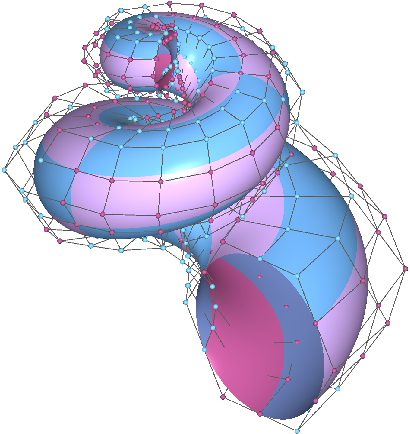
\includegraphics[scale = 1]{images/user_manual_logo.pdf}}}
        
        \bigskip{}
        \bigskip{}
	\end{flushright}
    
    
            
	\vspace*{\fill}
    
    \scriptsize{\noindent{}\CRed{Permission to make digital or hard copies of all or part of this work for personal or classroom use is granted without fee
        provided that copies are not made or distributed for profit or commercial advantage and that copies bear this notice and
        the full citation on the first page. Copyrights for components of this work owned by others than the author must be
        honored. Abstracting with credit is permitted. To copy otherwise, or republish, to post on servers, to redistribute to lists or to use in commercial/non-commercial applications
        requires prior specific permission and/or a fee.}}
    
	\newpage
\end{titlepage}

\frontmatter

\LRCornerWallPaper{0.25}{./images/phantom_BBU_2018.pdf}

\tableofcontents
\listoffigures

\mainmatter

\def\goldenratio{0.61803398875}
\begin{savequote}[\goldenratio\textwidth]
	\sffamily
	\footnotesize
	{
		\begin{center}
			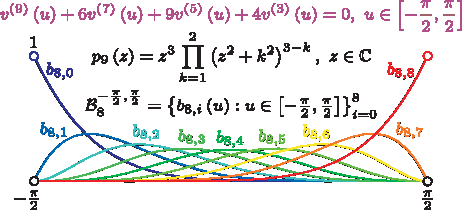
\includegraphics[height = 3.5cm]{images/theoretical_introduction.pdf}
		\end{center}
		\LinkColor{Extended Chebyshev spaces $\bullet$ Critical length for design $\bullet$ Constant-coefficient homogeneous linear differential equations  $\bullet$ Ordinary bases  $\bullet$ Normalized B-bases  $\bullet$ B-curves  $\bullet$ B-surfaces  $\bullet$ Construction and differentiation of normalized B-bases  $\bullet$  General order (or dimension) elevation  $\bullet$ General B-algorithm $\bullet$  General basis transformation  $\bullet$ Control point based exact description of ordinary integral curves and surface}
	}
\end{savequote}

\chapter{Theoretical introduction}

We propose a platform-independent multi-threaded function library that provides data structures to generate, differentiate and render both the ordinary basis and the normalized B-basis of a user-specified extended Chebyshev (EC) space that comprises the constants and can be identified with the solution space of a constant-coefficient homogeneous linear differential equation defined on a sufficiently small interval. Using the obtained normalized B-bases, our library can also generate, (partially) differentiate, modify and visualize a large family of so-called B-curves and tensor product B-surfaces. Moreover, the library also implements methods that can be used to perform dimension elevation, to subdivide B-curves and B-surfaces by means of de Casteljau-like B-algorithms, and to generate basis transformations for the B-representation of arbitrary integral curves and surfaces that  are described in traditional parametric form by means of the ordinary bases of the underlying EC spaces. Independently of the algebraic, exponential, trigonometric or mixed type of the applied EC space, the proposed library is numerically stable and efficient up to a reasonable dimension number and may be useful for academics and engineers in the fields of Approximation Theory, Computer Aided Geometric Design, Computer Graphics, Isogeometric and Numerical Analysis.


\section{Preliminaries}\label{sec:introduction}

In order to explain the possibilities of the proposed function library and to provide detailed implementation comments, we will use the following well-known notions. Let $n\geq1$ be a fixed integer and consider the extended Chebyshev (EC) system%
\begin{equation}
    \mathcal{F}_{n}^{\alpha,\beta}=\left\{  \varphi
    _{n,i}\left(  u\right)  :u\in\left[  \alpha,\beta\right]  \right\}  _{i=0}%
    ^{n},~\varphi_{n,0}	\equiv 1,~-\infty<\alpha<\beta<\infty\label{eq:ordinary_basis}%
\end{equation}
of basis functions in $C^{n}\left(  \left[  \alpha,\beta\right]  \right)  $,
i.e., by definition \citep{KarlinStudden1966}, for any integer $0\leq r\leq n$, any strictly increasing
sequence of knot values $\alpha\leq u_{0}<u_{1}<\ldots<u_{r}\leq\beta$, any
positive integers (or multiplicities) $\left\{  m_{k}\right\}  _{k=0}^{r}$
such that $\sum_{k=0}^{r}m_{k}=n+1$, and any real numbers $\left\{
\xi_{k,\ell}\right\}  _{k=0,~\ell=0}^{r,~m_{k}-1}$ there always exists a
unique function
\begin{equation}
    f:=\sum_{i=0}^{n}\lambda_{n,i}\varphi_{n,i}\in\mathbb{S}_{n}^{\alpha,\beta}:=\left\langle\mathcal{F}_{n}^{\alpha,\beta
    }\right\rangle:=\operatorname{span}\mathcal{F}_{n}^{\alpha,\beta},~\lambda_{n,i}\in\mathbb{R},~i=0,1,\ldots,n \label{eq:unique_solution}%
\end{equation}
that satisfies the conditions of the Hermite interpolation problem%
\begin{equation}
    f^{\left(  \ell\right)  }\left(  u_{k}\right)  =\xi_{k,\ell},~\ell
    =0,1,\ldots,m_{k}-1,~k=0,1,\ldots,r. \label{eq:Hermite_interpolation_problem}%
\end{equation}

In what follows, we assume that the sign-regular determinant of the coefficient
matrix of the linear system (\mref{eq:Hermite_interpolation_problem}) of
equations is strictly positive for any permissible parameter settings introduced above.
Under these circumstances, the vector space $\mathbb{S}_{n}^{\alpha,\beta}$ of functions is
called an EC space of dimension $n+1$. In terms of zeros, this
definition means that any non-zero element of $\mathbb{S}_{n}^{\alpha,\beta}$
vanishes at most $n$ times in the interval $\left[  \alpha,\beta\right]  $. Such spaces and their corresponding spline counterparts have been widely studied, consider, e.g.,\ articles \citep{Schumaker2007, Lyche1985,Pottmann1993,MazureLaurent1998,MainarPena1999,MainarPenaSanchez2001,LuWangYang2002,CarnicerMainarPena2004,MainarPena2004,CostantiniLycheManni2005,CarnicerMainarPena2007,MainarPena2010,Roth2015a,Roth2015b} and many other references therein. (Concerning the definition of EC spaces, the condition $1\equiv\varphi_{n,0}\in\mathbb{S}_{n}^{\alpha,\beta}$ would be not necessary, nevertheless we have included the constants in $\mathbb{S}_{n}^{\alpha,\beta}$ in order to ensure that all its bases can be normalized.)


Hereafter we will also refer to $\mathcal{F}_{n}^{\alpha,\beta}$ as the
ordinary basis of $\mathbb{S}_{n}^{\alpha,\beta}$ and we will also assume that the ($n$-dimensional) space
$
D\mathbb{S}_{n}^{\alpha,\beta}:=
\big\{
f^{\left(1\right)} 
: f \in \mathbb{S}_{n}^{\alpha,\beta}
\big\}
$
of the derivatives 
is also EC over the interval $\left[\alpha,\beta\right]$. Using \cite[Theorem
5.1]{CarnicerPena1995} and \cite[Theorem 4.1]{CarnicerMainarPena2004}, it follows that under these conditions the vector space $\mathbb{S}_{n}^{\alpha,\beta}$ also has a unique
strictly totally positive normalizable basis,
%\footnote{A basis $\left\{f_i\left(u\right):\left[\alpha,\beta\right]\right\}_{i=0}^{n}$ of $\mathbb{S}_{n}^{\alpha,\beta}$ is strictly totally positive, if all minors of all its collocation matrices $\left[f_i\left(u_j\right)\right]_{i=0,\,j=0}^{n,m}$ are strictly positive, where $\left\{u_j\right\}_{j=0}^m$ consists of arbitrary strictly increasing knot values within $\left[\alpha,\beta\right]$.},
called normalized B-basis
\begin{equation}
    \mathcal{B}_{n}^{\alpha,\beta}=\left\{  b_{n,i}\left(  u\right)  :u\in\left[
    \alpha,\beta\right]  \right\}  _{i=0}^{n} \label{eq:B-basis}%
\end{equation}
that apart from the identity%
\begin{equation}
    \sum_{i=0}^{n}b_{n,i}\left(  u\right)  \equiv1,~\forall u\in\left[
    \alpha,\beta\right]  \label{eq:partition_of_unity}%
\end{equation}
also fulfills the properties%
\begin{align}
    b_{n,0}\left(  \alpha\right)   &  =b_{n,n}\left(  \beta\right)
    =1,\label{eq:endpoint_interpolation}\\
    b_{n,i}^{\left(  j\right)  }\left(  \alpha\right)   &  =0,~j=0,\ldots
    ,i-1,~b_{n,i}^{\left(  i\right)  }\left(  \alpha\right)
    >0,\label{eq:Hermite_conditions_0}\\
    b_{n,i}^{\left(  j\right)  }\left(  \beta\right)   &  =0,~j=0,1,\ldots
    ,n-1-i,~\left(  -1\right)  ^{n-i}b_{n,i}^{\left(  n-i\right)  }\left(
    \beta\right)  >0 \label{eq:Hermite_conditions_alpha}%
\end{align}
conform \cite[Theorem 5.1]{CarnicerPena1995} and \cite[Equation (3.6)]{Mazure1999}. (In order to avoid ambiguity, in case of some figures we will also use the notation $\overline{\mathcal{F}}_n^{\alpha,\beta}$ instead of $\mathcal{B}_n^{\alpha,\beta}$.)

All algorithms that will be presented in the forthcoming sections are valid in case of any EC space $\mathbb{S}_n^{\alpha, \beta}$ that fulfills all conditions above, however in case of their C++ and OpenGL based implementation we always assume that $\mathbb{S}_n^{\alpha, \beta}$ can be identified with the solution space of the constant-coefficient homogeneous linear differential equation
\begin{equation}
    \sum_{i=0}^{n+1}\gamma_{i}v^{\left(  i\right)  }\left(  u\right)=0,~\gamma_{i}\in\mathbb{R},~u\in\left[  \alpha,\beta\right]  
    \label{eq:differential_equation}
\end{equation} 
of order $n+1$. Such a solution space:
\begin{itemize}
    \item 
    is translation invariant and it is spanned by those ordinary basis functions that are generated by the (higher order) zeros of the characteristic polynomial
    \begin{equation}
        p_{n+1}\left(  z\right) =\sum_{i=0}^{n+1}\gamma_{i}z^{i},~z\in \mathbb{C}
        \label{eq:characteristic_polynomial}%
    \end{equation}
    associated with the differential equation (\mref{eq:differential_equation}) (naturally, in order to ensure that $\varphi_{n,0}\equiv 1 \in \mathbb{S}_n^{\alpha,\beta}$, we will assume that $z=0$ is at least a first order zero of (\mref{eq:characteristic_polynomial}));
    
    \item
    is of class $C^{\infty}\left(\left[\alpha,\beta\right]\right)$ and is EC on intervals of sufficiently small length $\beta-\alpha \in \left(0,\ell_n\right)$, where the so-called critical length $\ell_n > 0$ (i.e., the supremum of the lengths of the intervals on which the given space is EC) can be determined as follows (see \cite[Proposition 3.1]{CarnicerMainarPena2004}):
    \begin{itemize}
        \item
        let
        \begin{equation}
            W_{\left[  v_{n,0},v_{n,1},\ldots,v_{n,n}\right]  }\left(  u\right)  :=
            \left[
            v_{n,i}^{\left(j\right)}\left(u\right)
            \right]_{i=0,~j=0}^{n,~n},~u\in\left[\alpha,\beta\right]
            \label{eq:forward_Wronskian}
        \end{equation}
        be the Wronskian matrix of those particular integrals
        \begin{equation}
            v_{n,i}:=\sum_{k=0}^{n}\rho_{i,k}\varphi_{n,k}\in\mathbb{S}_{n}^{\alpha,\beta
            },~\left\{\rho_{i,k}\right\}_{k=0}^{n}\subset\mathbb{R},~i=0,1,\ldots,n\label{eq:particular_integrals}%
        \end{equation}
        of (\mref{eq:differential_equation}) which correspond to the boundary conditions%
        \begin{equation}
            \def\arraystretch{1.3}
            \left\{
            \begin{array}{rcl}
                v_{n,i}^{\left(  j\right)  }\left(  \alpha\right)    & = & 0,~j=0,\ldots,i-1,\\
                v_{n,i}^{\left(  i\right)  }\left(  \alpha\right)    & = & 1,\\
                v_{n,i}^{\left(  j\right)  }\left(  \beta\right)    & =& 0 ,~j=0,\ldots,n-1-i,
            \end{array}
            \right.
            \def\arraystretch{1.0}
            \label{eq:boundary_conditions}
        \end{equation}
        i.e., the system $\left\{  v_{n,i}\left(  u\right)  :u\in\left[
        \alpha,\beta\right]  \right\}  _{i=0}^{n}$ is a bicanonical basis on the interval $\left[\alpha, \beta\right]$ such that the Wronskian (\mref{eq:forward_Wronskian}) at $u=\alpha$ is a
        lower triangular matrix with positive (unit) diagonal entries;
        \item
        consider the functions (or Wronskian determinants)%
        \begin{align}
            w_{n,i}\left(  u\right)  &:=\det W_{\left[  v_{n,i},v_{n,i+1},\ldots
                ,v_{n,n}\right]  }\left(  u\right)  ,~i=
            \left\lfloor \tfrac{n}{2}\right\rfloor +1,\ldots
            ,n,\label{eq:Wronskian_determinants}
            \\
            \theta_{n,i}\left(u\right) &:= \left(-1\right)^{n\left(n+1-i\right)}\det W_{\left[  v_{n,i},v_{n,i+1},\ldots,v_{n,n}\right]  }\left(  -u\right),~i=
            \left\lfloor \tfrac{n}{2}\right\rfloor +1,\ldots,n,
        \end{align}
        define the critical length%
        \begin{equation}
            \ell_{n}:=\min_{i=\left\lfloor \frac{n}{2}\right\rfloor +1,\ldots
                ,n}\min\left\{  \left\vert u - \alpha\right\vert :w_{n,i}\left(  u\right)
            =0\text{ or } \theta_{n,i}\left(u\right)=0,~u\neq\alpha\right\}
            \label{eq:critical_length}
        \end{equation}
        (we write $\ell_{n}=+\infty$ whenever the Wronskian determinants
        (\mref{eq:Wronskian_determinants}) do not have real zeros other than $\alpha$, moreover $\ell_{n}$ is infinite whenever the characteristic polynomial (\mref{eq:characteristic_polynomial}) has only real roots, otherwise it is finite a number that, in general, also depends on parameters resulting from the differential equation (\mref{eq:differential_equation}), i.e., on the real and imaginary parts of the complex zeros of the characteristic polynomial (\mref{eq:characteristic_polynomial})).
    \end{itemize}
\end{itemize}

We will denote the critical length of the derivative space $D\mathbb{S}_{n}^{\alpha,\beta}$ by $\ell_n^{\prime}$ and, in order to ensure that $\mathbb{S}_n^{\alpha, \beta}$ is an EC space that also possesses a unique normalized B-basis (see \cite[Theorem 4.1 and Corollary 4.1]{CarnicerMainarPena2004}), \textit{from hereon we always assume that} $\beta \in \left(\alpha, \alpha + \ell_n^{\prime}\right)$. (The interval length $\beta - \alpha \in \left(0,\ell_n^{\prime}\right)$ can be considered as a shape or tension parameter. In order to avoid ambiguity, instead of $\ell_{n}$ and $\ell_n^{\prime}$, in some cases, we will also use the notations $\ell\left( \mathbb{S}_n^{\alpha,\beta}\right)$ and $\ell^{\prime}\left( \mathbb{S}_n^{\alpha,\beta}\right):=\ell\left(D\mathbb{S}_{n}^{\alpha,\beta}\right)$, respectively.) Following \cite[p.\ 67]{CarnicerMainarPena2004}, we will also refer to $\ell_n^{\prime}$ as \textit{critical length for design}.

\begin{remark}[Concerning the endpoints of the definition domain]
    Since the un\-der\-ly\-ing vec\-tor space $\mathbb{S}_n^{\alpha,\beta}$ is trans\-la\-tion invariant, it would be sufficient to study the properties of such spaces on intervals of the form $[0,h]$, where $h \in \left(0,\ell_n^{\prime}\right)$ and, consequently, the notation $\mathbb{S}_{n}^{\alpha,\beta}$ could be simplified to $\mathbb{S}_{n}^{h}$. Nevertheless, due to flexibility and some implementation details which may appear, e.g.,\ in case of the control point based exact description (i.e., B-representation) of ordinary integral curves defined on intervals of appropriate length, we have designed/implemented all proposed algorithms on the interval $\left[\alpha,\beta\right]$, where $\beta - \alpha \in \left(0,\ell_n^{\prime}\right)$. In this way, during programming, users will have more comfort, e.g., they do not have to deal with phase changes.
\end{remark}  

As we will see, the proposed algorithms do not assume that the characteristic polynomial (\mref{eq:characteristic_polynomial}) is an either odd or even function, but if this the case, the underlying EC space will also be reflection invariant, i.e., if $\mathbb{S}_n^{\alpha,\beta}$ denotes the solution space of (\mref{eq:differential_equation}), $v\in\mathbb{S}_n^{\alpha,\beta}$ and $x\in\mathbb{R}$ is fixed, then $v\left(u - x\right)$ also belongs to  $\mathbb{S}_n^{\alpha,\beta}$, moreover the normalized B-basis functions (\mref{eq:B-basis}) will share the symmetry property 
\begin{equation}
    b_{n,i}\left(u\right)=b_{n,n-i}\left(\alpha + \beta - u\right),~\forall u \in \left[\alpha, \beta\right],~i=0,1,\ldots,\left\lfloor \tfrac{n}{2}\right\rfloor.
    \label{eq:symmetry}
\end{equation}
In this case, the critical length (\mref{eq:critical_length}) can be determined (see \cite[Proposition 3.2]{CarnicerMainarPena2004}) by means of the simpler formula
\begin{equation}
    \ell_{n}:=\min_{i=\left\lfloor \frac{n}{2}\right\rfloor +1,\ldots
        ,n}\min\left\{  \left\vert u - \alpha\right\vert :w_{n,i}\left(  u\right)
    =0,~u\neq\alpha\right\}.
    \label{eq:critical_length_reflection_invariant}
\end{equation}


Based on both original and existing theoretical results, the main objective of the manuscript is to propose and implement general algorithms into a robust and flexible OpenGL and C++ based multi-threaded function library that can be used: 
\begin{itemize}
    \item 
    to automatically generate and evaluate the derivatives of any order of both the ordinary basis and the normalized B-basis of a not necessarily reflection invariant EC space that comprises the constants, can be identified with the translation invariant solution space of the differential equation (\mref{eq:differential_equation}) and whose derivative space is also EC;
    
    \item
    to describe, generate, manipulate and render so-called B-curves defined as convex combinations of control points and normalized B-basis functions;
    
    \item
    to generate, manipulate and render so-called B-surfaces defined as tensor products of B-curves;
    
    \item
    to elevate the dimension of the underlying EC space(s) and consequently the order(s) of the B-curve (surface) that is rendered;
    
    \item
    to subdivide B-curves by means of general B-algorithms implied by the normalized B-basis of the given EC space and to extend this subdivision technique to B-surfaces;
    
    \item
    to generate transformations matrices that map the normalized B-bases of the applied EC spaces to their ordinary bases, in order to ensure control point configurations for the exact B-representation of large classes of integral curves and surfaces that are described in traditional parametric form by means of the ordinary bases of the used EC spaces.
\end{itemize}

\section{Proposed algorithms}\label{sec:proposed_algorithms}

The full implementation details of the proposed function library and test cases that exemplify the usage of our algorithms appear in Chapters \mref{ch:Full_implementation_details} and \mref{ch:Usage_examples}, respectively. After each mathematical notion, theorem or algorithm, this section also includes brief cross references both to the corresponding full implementation details and to the examples that should be considered by the reader. We deliberately omitted the proofs of our theoretical results from this user manual, however they can be found in the paper \citep{Roth2018a}. In order to formulate the input and output of our algorithms, we define the following control point based integral curves and surfaces.

\begin{definition}[B-curves]
    The convex combination 
    \begin{equation}
    \mathbf{c}_{n}\left(  u\right)  =\sum_{i=0}^{n}\mathbf{p}_{i}b_{n,i}\left(
    u\right)  ,~ u\in\left[  \alpha,\beta\right],~0<\beta-\alpha < \ell^{\prime}\left(\mathbb{S}_{n}^{\alpha,\beta}\right)  ,~\mathbf{p}_{i}=\left[
    p_{i}^{\ell}\right]  _{\ell=0}^{\delta-1}\in%
    \mathbb{R}
    ^{\delta},\,\delta \geq 2 \label{eq:B_curve}%
    \end{equation}
    described by means of the normalized B-basis (\mref{eq:B-basis}) is called a B-curve of order $n$, where $\left[\mathbf{p}_i\right]_{i=0}^n$ denotes its control polygon.
\end{definition}

\noindent{}\CRed{\textbf{Brief implementation details.}} In case of our implementation B-curves are represented by the class \CBlue{BCurve3} that is derived from the base abstract class \CBlue{LinearCombination3}. The diagrams of these data structures are illustrated in Figs.\ \mref{fig:UMLLinearCombination3} and \mref{fig:UMLBCurve3}, while their declarations and definitions can be found in Listing pairs \mref{src:LinearCombinations3.h}--\mref{src:LinearCombinations3.cpp} and \mref{src:BCurves3.h}--\mref{src:BCurves3.cpp}, respectively.

\bigskip{}

\noindent{}\CRed{\textbf{Examples to consider.}} Listings \mref{src:GLWidgetDefineEvaluateDifferentiateManipulateRenderBCurves.h}--\mref{src:GLWidgetDefineEvaluateDifferentiateManipulateRenderBCurves.cpp} and Fig.\ \mref{fig:B-curve_operations} of Subsection \mref{subsec:B-curve_generation_order_elevation_and_subdivision} provide examples for the definition, generation, evaluation, differentiation, order elevation, subdivision and rendering of different types of B-curves. Listings \mref{src:GLWidget_exmp_03.h}--\mref{src:GLWidget_exmp_03.cpp} and Fig.\ \mref{fig:logarithmic_spiral} of Subsection \mref{subsec:B_representation_of_ordinary_integral_curves} provide an example for the control point based exact description (or B-representation) of integral curves given in traditional (i.e., ordinary) parametric form.

\begin{definition}[B-surfaces]
    Denoting by
    \[
    \mathcal{B}_{n_r}^{\alpha_r, \beta_r}
    =
    \left\{
    b_{n_r,i_r}\left(u_r;\alpha_r,\beta_r\right): u_r \in \left[\alpha_r, \beta_r\right]
    \right\}_{i_r=0}^{n_r},~0<\beta_r-\alpha_r < \ell^{\prime}\left(\mathbb{S}_{n_r}^{\alpha_r,\beta_r}\right),~r=0,1
    \]
    the normalized B-bases of some EC spaces and using the tensor product of curves of type (\mref{eq:B_curve}), one can define the B-surface 
    \begin{equation}
    \label{eq:B-surface}
    \mathbf{s}_{n_0,n_1}\left(u_0,u_1\right)
    =
    \sum_{i_0=0}^{n_0} \sum_{i_1 = 0}^{n_1}
    \mathbf{p}_{i_0,i_1}
    b_{n_0,i_0}\left(u_0;\alpha_0, \beta_0\right)
    b_{n_1,i_1}\left(u_1;\alpha_1, \beta_1\right),\:\mathbf{p}_{i_0,i_1}=\left[p_{i_0,i_1}^{\ell}\right]_{\ell=0}^2\in\mathbb{R}^3
    \end{equation}
    of order $\left(n_0,n_1\right)$, where the matrix $\left[\mathbf{p}_{i_0,i_1}\right]_{i_0=0,\,i_1=0}^{n_0,\,n_1}$ forms a control net.
\end{definition}

\noindent{}\CRed{\textbf{Brief implementation details.}} The proposed function library represents B-surfaces by the class \CBlue{BSurface3} that is derived from the base abstract class \CBlue{TensorProductSurface3}. The diagrams of these types are illustrated in Figs.\ \mref{fig:UMLTensorProductSurface3} and \mref{fig:UMLBSurface3}, while their declarations and definitions can be found in Listing pairs \mref{src:TensorProductSurfaces3.h}--\mref{src:TensorProductSurfaces3.cpp} and \mref{src:BSurfaces3.h}--\mref{src:BSurfaces3.cpp}, respectively.

\bigskip{}

\noindent{}\CRed{\textbf{Examples to consider.}} Listings \mref{src:GLWidgetTestingBSurfaceOperations.h}--\mref{src:GLWidgetTestingBSurfaceOperations.cpp} and Figs.\ \mref{fig:B_surface_order_elevation}--\mref{fig:B_surface_subdivision_v} of Subsection \mref{subsec:B-surface_generation_order_elevation_and_subdivision} provide examples for the definition, generation, evaluation, differentiation, order elevation, subdivision and rendering of different types of B-surfaces. Listings \mref{src:GLWidgetTestingBSurfaceOperations.h}--\mref{src:GLWidgetTestingBSurfaceOperations.cpp} and Figs.\ 
\mref{fig:control_point_based_exact_description_snail_tau_2}-- \mref{fig:isoparametric_lines_user_manual} of Subsection \mref{subsec:B-representation_of_ordinary_integral_surfaces} give examples for both the control point based exact description (or B-representation) of integral surfaces given in traditional (i.e., ordinary) parametric form and the generation, evaluation, differentiation and rendering of isoparametric lines of B-surfaces.

\subsection{Construction and differentiation of normalized B-basis functions in a large class of EC spaces}\label{subsec:construction}

As already stated in Section \mref{sec:introduction}, our implementation assumes that the underlying EC space $\mathbb{S}_{n}^{\alpha,\beta}$ corresponds to the solution space of a constant-coefficient homogeneous linear differential equation of type (\mref{eq:differential_equation}), where $\beta-\alpha \in \left(0,\ell_n^{\prime}\right)$. This is not necessary for the correctness of the algorithms that will be presented in the forthcoming sections. The only reason for this additional assumption is the fact that in this case we have the possibility to handle a large family of (mixed) EC spaces in a unified way.

For example, if $\mathbf{i}=\sqrt{-1}$, $a, b \in \mathbb{R}$ and $z=a+\mathbf{i}b$ is an $m$th order ($m\geq 1$) zero of the characteristic polynomial (\mref{eq:characteristic_polynomial}), then based on its real and imaginary parts one has that:
\begin{itemize}
    \item
    if $a,b\in\mathbb{R}\setminus\left\{0\right\}$, the conjugate complex number $\overline{z}$ is also a root of multiplicity $m$ and consequently one obtains an algebraic-exponential-trigonometric (AET) mixed EC subspace
    \begin{equation}
    \label{eq:AET}
    \left\langle
    \left\{
    u^r e^{au} \cos\left(bu\right),
    u^r e^{au} \sin\left(bu\right):
    u \in \left[\alpha,\beta\right]
    \right\}_{r=0}^{m-1}
    \right\rangle \subseteq \mathbb{S}_n^{\alpha,\beta};
    \end{equation}
    \item
    if $a \neq 0$, but $b=0$, then one has the
    algebraic-exponential (AE) mixed EC subspace
    \begin{equation}
    \label{eq:AE}
    \left\langle
    \left\{
    u^r e^{au} : u \in \left[\alpha,\beta\right]
    \right\}_{r=0}^{m-1}
    \right\rangle \subseteq \mathbb{S}_n^{\alpha,\beta};
    \end{equation}
    \item
    if $a = 0$, but $b \neq 0$, then one obtains the algebraic-trigonometric (AT) mixed EC subspace
    \begin{equation}
    \label{eq:AT}
    \left\langle
    \left\{
    u^r \cos\left(bu\right),
    u^r \sin\left(bu\right):
    u \in \left[\alpha,\beta\right]
    \right\}_{r=0}^{m-1}
    \right\rangle \subseteq \mathbb{S}_n^{\alpha,\beta};
    \end{equation}
    \item
    if $a=b=0$ then one has the polynomial (P) EC subspace
    \begin{equation}
    \label{eq:P}	
    \left\langle
    \left\{
    u^r : u \in \left[\alpha,\beta\right]
    \right\}_{r=0}^{m-1}
    \right\rangle \subseteq \mathbb{S}_n^{\alpha,\beta}.
    \end{equation}
\end{itemize}
This means that one can easily define ordinary (mixed) basis functions by simply specifying the factorization of the characteristic polynomial (\mref{eq:characteristic_polynomial}), i.e., one can create (mixed) EC spaces at run-time in an interactive way. As we will see, the zeroth and higher order (endpoint) derivatives of the ordinary basis function will play an important role in case of all proposed algorithms. In case of the aforementioned (mixed) EC subspaces one can overload function operators to compute the required derivatives for arbitrarily fixed orders -- this possibility also motivates our assumption on the structure of the underlying EC space. Moreover, in real-world engineering, computer-aided design and manufacturing applications, usually one defines traditional parametric curves and surfaces by means of the ordinary basis functions presented above and, in our opinion, it would be nice to have a unified framework in which -- apart from general order elevation and subdivision -- one is also able to describe exactly important curves and surfaces by using control points and normalized B-basis functions.

In order to have normalizable bases in the vector space $\mathbb{S}_n^{\alpha,\beta}$, we also have to assume that $z=0$ is at least a first order zero of the characteristic polynomial (\mref{eq:characteristic_polynomial}).

Once we have created an EC space of type $\mathbb{S}_n^{\alpha,\beta}$ by defining its ordinary basis $\mathcal{F}_n^{\alpha,\beta}$ (where $\beta-\alpha \in \left(0,\ell_n^{\prime}\right)$), we also have to generate its unique normalized B-basis $\mathcal{B}_n^{\alpha,\beta}$.
In order to achieve this and to be as self-contained as possible, we recall the construction process \citep{CarnicerMainarPena2004} of $\mathcal{B}_n^{\alpha,\beta}$. As we will see, the steps of this process can be fully implemented in case of the aforementioned (mixed) EC spaces.

Consider the bicanonical basis $\left\{v_{n,i}\left(u\right):u\in\left[\alpha,\beta\right]\right\}_{i=0}^{n}$ formed by the particular integrals (\mref{eq:particular_integrals}) determined by the boundary conditions (\mref{eq:boundary_conditions}). Let $W_{\left[v_{n,n},v_{n,n-1},\ldots,v_{n,0}\right]  }\left(  \beta\right)  $ be the Wronskian matrix of the reverse ordered system
$\{  v_{n,n-i}\left(  u\right)  :\allowbreak{}u\in\left[  \alpha,\beta\right]  \}
_{i=0}^{n}$ at the parameter value $u=\beta$ and obtain its Doolittle-type $LU$ factorization %
\begin{equation}
L\cdot U=W_{\left[  v_{n,n},v_{n,n-1},\ldots,v_{n,0}\right]  }\left(
\beta\right),
\label{eq:LU_factorization_of_reversed_system}
\end{equation}
where $L$ is a lower triangular matrix with unit diagonal,
while $U$ is a non-singular upper triangular matrix. Calculate the inverse matrices%
\[
U^{-1}:=\left[
\begin{array}
[c]{cccc}%
\mu_{0,0} & \mu_{0,1} & \cdots & \mu_{0,n}\\
0 & \mu_{1,1} & \cdots & \mu_{1,n}\\
\vdots & \vdots & \ddots & \vdots\\
0 & 0 & \cdots & \mu_{n,n}%
\end{array}
\right]  ,~L^{-1}:=\left[
\begin{array}
[c]{cccc}%
\lambda_{0,0} & 0 & \cdots & 0\\
\lambda_{1,0} & \lambda_{1,1} & \cdots & 0\\
\vdots & \vdots & \ddots & \vdots\\
\lambda_{n,0} & \lambda_{n,1} & \cdots & \lambda_{n,n}%
\end{array}
\right]
\]
and construct the normalized B-basis%
\begin{equation}
\mathcal{B}_{n}^{\alpha,\beta}=\left\{  b_{n,i}\left(  u\right)  =\lambda
_{n-i,0}\widetilde{b}_{n,i}\left(  u\right)  :u\in\left[  \alpha,\beta\right]
\right\}  _{i=0}^{n}\label{eq:construction}%
\end{equation}
defined by%
\[
\left[
\begin{array}
[c]{cccc}%
\widetilde{b}_{n,n}\left(  u\right)   & \widetilde{b}_{n,n-1}\left(
u\right)   & \cdots & \widetilde{b}_{0}\left(
u\right)
\end{array}
\right]  :=\left[
\begin{array}
[c]{cccc}%
v_{n,n}\left(  u\right)   & v_{n,n-1}\left(  u\right)   & \cdots &
v_{n,0}\left(  u\right)
\end{array}
\right]  \cdot U^{-1}%
\]
and%
\[
\left[
\begin{array}
[c]{cccc}%
\lambda_{0,0} & \lambda_{1,0} & \cdots & \lambda_{n,0}%
\end{array}
\right]  ^{T}:=L^{-1}\cdot\left[
\begin{array}
[c]{cccc}%
1 & 0 & \cdots & 0
\end{array}
\right]  ^{T}.
\]

If the characteristic polynomial (\mref{eq:characteristic_polynomial}) is an either even or odd function, then the underlying EC space $\mathbb{S}_{n}^{\alpha,\beta}$ is invariant under reflections, and in this special case one obtains the symmetry (\mref{eq:symmetry}), i.e., we only need to determine the half of the basis functions
(\mref{eq:construction}). 

\begin{remark}[An alternative construction]The non-negative bicanonical basis $\big\{v_{n,i}:u\in[\alpha,\allowbreak{}\beta]\big\}_{i=0}^{n}$ formed by the particular integrals (\mref{eq:particular_integrals}) is a B-basis of the EC space $\mathbb{S}_n^{\alpha,\beta}$ (see \cite[Theorem 2.4/(ii)]{CarnicerMainarPena2004}). Compared with the previously described $LU$ decomposition based method, this B-basis can also be normalized by means of the normalizing coefficients
    \begin{equation}
    c_{n,i}:=-\sum_{r=0}^{i-1} c_{n,r} v_{n,r}^{\left(i\right)}\left(\alpha\right),~i=1,\ldots,n,
    \label{eq:alternative_normalizing_coefficients}
    \end{equation}
    where $c_{n,0}=1$. This means that the unique normalized B-basis functions of the underlying EC space $\mathbb{S}_{n}^{\alpha,\beta}$ could also be determined as the linear combinations
    \begin{equation}
    b_{n,i}\left(u\right) := \sum_{i=0}^{n} c_{n,i} v_{n,i}\left(u\right),~u \in \left[\alpha,\beta\right],~i=0,1,\ldots,n.
    \label{eq:alternative_construction_process}
    \end{equation}
    Although the construction process (\mref{eq:alternative_normalizing_coefficients})--(\mref{eq:alternative_construction_process}) requires less computational effort, several numerical tests show that this alternative method is numerically less stable than (\mref{eq:LU_factorization_of_reversed_system})--(\mref{eq:construction}). 
\end{remark}

Summarizing the calculations of the current section, we can state the next corollary that will be very important both in the formulation and in the implementation of all proposed algorithms.

\begin{corollary}[Differentiation of normalized B-basis functions]\label{cor:B_basis_derivatives}
    In general, the zeroth and higher order differentiation of the constructed normalized B-basis functions (\mref{eq:construction}) can be reduced to the evaluation of formulas
    \begin{align}
    b_{n,n-i}^{\left(  j\right)  }\left(  u\right)    
    & =\lambda_{i,0}%
   	\widetilde{b}_{n,n-i}^{\left(  j\right)  }\left(  u\right)  \nonumber\\
   	& 
    =
    \lambda_{i,0}\sum_{r=0}^{i}\mu_{r,i}v_{n,n-r}^{\left(  j\right)  }\left(
   	u\right)  \nonumber\\
    & =\lambda_{i,0}\sum_{r=0}^{i}\mu_{r,i}\sum_{k=0}^{n}\rho_{n-r,k}\varphi
    _{n,k}^{\left(  j\right)  }\left(  u\right)  ,~\forall u \in \left[\alpha,\beta\right],~i=0,1,\ldots,n.
    \label{eq:mixed_b_derivatives}
    \end{align}
    Naturally, if the underlying EC space is reflection invariant, then formulas (\mref{eq:mixed_b_derivatives}) have to be applied only for indices $i=0,1,\ldots,\left\lfloor \frac{n}{2}\right\rfloor$, since in this special case one also has that
    \begin{align}
    b_{n,i}^{\left(  j\right)  }\left(  u\right)    & =\left(  -1\right)
    ^{j}b_{n,n-i}^{\left(  j\right)  }\left(  \alpha+\beta-u\right)  ,~\forall u \in \left[\alpha, \beta\right],~i=0,1,\ldots
    ,\left\lfloor \tfrac{n}{2}\right\rfloor.
    \label{eq:mixed_b_symmetric_derivatives}
    \end{align}
\end{corollary}

\noindent{}\CRed{\textbf{Brief implementation details.}} Classes \CBlue{CharacteristicPolynomial} and \CBlue{ECSpace}, that provide interfaces for the factorization management of the general characteristic polynomial (\mref{eq:characteristic_polynomial}) and for the generation of the EC space implied by it, are illustrated in Figs.\ \mref{fig:UMLCharacteristicPolynomial} and \mref{fig:UMLECSpace}, while their declaration can be found in Listings \mref{src:CharacteristicPolynomials.h} and \mref{src:ECSpaces.h}, respectively. The full implementation details of these classes are presented in Listings \mref{src:CharacteristicPolynomials.cpp} and \mref{src:ECSpaces.cpp}, respectively. For example, the construction process
((\mref{eq:forward_Wronskian})--(\mref{eq:boundary_conditions}), (\mref{eq:LU_factorization_of_reversed_system})--(\mref{eq:construction})) of the normalized B-basis functions of the underlying EC space and their differentiation formulas (\mref{eq:mixed_b_derivatives}) are implemented in lines \mref{ECSpace::updateBothOrdinaryAndNNBBases::start}--\mref{ECSpace::updateBothOrdinaryAndNNBBases::end} and \mref{ECSpace::operator()::start}--\mref{ECSpace::operator()::end} of Listing \mref{src:ECSpaces.cpp}, respectively.

\bigskip{}

\noindent{}\CRed{\textbf{Examples to consider.}} Deriving from the base class \CBlue{ECSpace}, one can define special (like pure poly\-no\-mi\-al/trig\-o\-no\-met\-ric/hyperbolic and mixed exponential-trigonometric or algebraic-\{trig\-o\-no\-met\-ric/hy\-per\-bo\-lic/ex\-po\-nen\-tial-trigonometric\}) EC spaces as it is presented by several examples in Listings \mref{src:SpecializedECSpaces.h} and \mref{src:SpecializedECSpaces.cpp} of Section \mref{sec:Defining_and_using specialized_EC_spaces}. In Listings \mref{src:GLWidgetDifferentiatingAndRenderingBasisFunctions.h} and \mref{src:GLWidgetDifferentiatingAndRenderingBasisFunctions.cpp} of Section \mref{sec:Differentiating_and_rendering_basis_functions}, we also provided examples for the evaluation, differentiation and rendering of both the ordinary basis and the normalized B-basis of different types of EC spaces. A possible output of these source codes is illustrated in Fig.\ \mref{fig:differentiation_and_rendering_of_B_bases}.



\subsection{General dimension and order elevation}

Consider the EC spaces $\mathbb{S}_n^{\alpha,\beta}$ and $\mathbb{S}_{n+1}^{\alpha,\beta}$ such that $1\in \mathbb{S}_n^{\alpha,\beta} \subset \mathbb{S}_{n+1}^{\alpha,\beta}$ and assume that spaces $D\mathbb{S}_{n}^{\alpha,\beta}$ and $D\mathbb{S}_{n+1}^{\alpha,\beta}$ of the derivatives are also EC on $\left[\alpha,\beta\right]$, i.e., $
0<\beta-\alpha<\min\left\{\ell^{\prime}\left(\mathbb{S}_{n}^{\alpha,\beta}\right),\ell^{\prime}\left(\mathbb{S}_{n+1}^{\alpha,\beta}\right)\right\},
$
furthermore let us denote their unique normalized B-bases by $\left\{b_{n,i}\left(u\right):u\in\left[\alpha,\beta\right]\right\}_{i=0}^n$ and $\big\{b_{n+1,i}\left(u\right):u\in\left[\alpha,\beta\right]\big\}_{i=0}^{n+1}$, respectively. Following the results of \cite[Theorem 3.1]{MazureLaurent1998} and, as a slight difference, considering both endpoints of the definition domain $\left[\alpha, \beta\right]$ in order to minimize the maximal differentiation order of the lower and higher order normalized B-basis functions, one can state the next lemma.

\begin{lemma}[General order elevation, \textnormal{\citep{MazureLaurent1998}}]
    \label{lem:general_order_elevation}
    Using the notations of the section, the $n$th order B-curve (\mref{eq:B_curve}) fulfills the identity
    $$
    \mathbf{c}_n\left(u\right)=\sum_{i=0}^n \mathbf{p}_i b_{n,i}\left(u\right)\equiv\sum_{i=0}^{n+1}\mathbf{p}_{1,i} b_{n+1,i}\left(u\right)=:\mathbf{c}_{n+1}\left(u\right),~\forall u \in \left[\alpha, \beta\right],
    $$
    where $\mathbf{p}_{1,0} = \mathbf{p}_{0}, ~\mathbf{p}_{1,n+1} = \mathbf{p}_n$ and
    \begin{align}
    \mathbf{p}_{1,i} 
    &= 
    \left(
    1-
    \frac
    {
        b_{n,i}^{\left(i\right)}\left(\alpha\right)
    }
    {
        b_{n+1,i}^{\left(i\right)}\left(\alpha\right)
    }
    \right)
    \mathbf{p}_{i-1}
    +
    \frac
    {
        b_{n,i}^{\left(i\right)}\left(\alpha\right)
    }
    {
        b_{n+1,i}^{\left(i\right)}\left(\alpha\right)
    }
    \mathbf{p}_i,~i=1,\ldots,\left\lfloor \tfrac{n}{2} \right\rfloor,
    \label{eq:order_elevation_inner_points_first_half}
    \\
    \mathbf{p}_{1,n+1-i} 
    & = \frac{b_{n,n-i}^{\left(i\right)}\left(\beta\right)}{b_{n+1,n+1-i}^{\left(i\right)}\left(\beta\right)} \mathbf{p}_{n-i} + 
    \left(1-\frac{b_{n,n-i}^{\left(i\right)}\left(\beta\right)}{b_{n+1,n+1-i}^{\left(i\right)}\left(\beta\right)}\right)\mathbf{p}_{n+1-i},~i=1,\ldots,\left\lfloor\tfrac{n+1}{2}\right\rfloor.
    \label{eq:order_elevation_inner_points_second_half}
    \end{align}
\end{lemma}


Although Lemma \mref{lem:general_order_elevation} is valid for any nested EC spaces that fulfill the conditions $1\in \mathbb{S}_n^{\alpha,\beta} \subset \mathbb{S}_{n+1}^{\alpha,\beta}$ and for which the derivative spaces $D\mathbb{S}_{n}^{\alpha,\beta}$ and $D\mathbb{S}_{n+1}^{\alpha,\beta}$ are also EC, in case of our implementation, we always assume that the higher dimensional EC space $\mathbb{S}_{n+1}^{\alpha,\beta}$ can also be identified with the solution space of a constant-coefficient homogeneous linear differential equation.

\bigskip{} 

\noindent{}\CRed{\textbf{Brief implementation details.}} The declaration and definition of the class \CBlue{BCurve3} that represents B-curves of type (\mref{eq:B_curve}) can be found in Listings \mref{src:BCurves3.h} and \mref{src:BCurves3.cpp}, respectively. For example, formulas (\mref{eq:order_elevation_inner_points_first_half})--(\mref{eq:order_elevation_inner_points_second_half}) of the general order elevation are implemented in lines \mref{BCurve3::performOrderElevation::start}--\mref{BCurve3::performOrderElevation::end} of Listing \mref{src:BCurves3.cpp}. Naturally, the results of Lemma \mref{lem:general_order_elevation} can also be extended to the general order elevation of B-surfaces of type (\mref{eq:B-surface}) and our function library ensures this possibility as well: the declaration and definition of the class \CBlue{BSurface3} can be found in Listings \mref{src:BSurfaces3.h} and \mref{src:BSurfaces3.cpp}, respectively, while the order elevation of B-surfaces is implemented in lines \mref{BSurface3::performOrderElevation::start}--\mref{BSurface3::performOrderElevation::end} of Listing \mref{src:BSurfaces3.cpp}.

\bigskip{}

\noindent{}\CRed{\textbf{Examples to consider.}} Examples for the order elevation of different types of B-curves and B-surfaces can be found in Listing pairs \mref{src:GLWidgetDefineEvaluateDifferentiateManipulateRenderBCurves.h}--\mref{src:GLWidgetDefineEvaluateDifferentiateManipulateRenderBCurves.cpp} and \mref{src:GLWidgetTestingBSurfaceOperations.h}--\mref{src:GLWidgetTestingBSurfaceOperations.cpp}, respectively. Figs.\ \mref{fig:B-curve_operations} and \mref{fig:B_surface_order_elevation}--\mref{fig:color_schemes} illustrate order elevated B-curves and B-surfaces, respectively, that were obtained as possible outputs of these source codes.


\subsection{General B-algorithm}\label{subsec:general_B_algorithm}

Theoretically, every normalized B-basis implies a B-algorithm for the subdivision of B-curves like (\mref{eq:B_curve}), i.e., for an arbitrarily fixed parameter value $\gamma \in \left(\alpha, \beta\right)$ there exists a recursive corner cutting de Casteljau-like algorithm that starts with the initial conditions %
$
\mathbf{p}_i^0\left(\gamma\right)\equiv\mathbf{p}_i,~ i=0,1,\ldots,n
$
and recursively defines the subdivision points
\begin{equation}
\label{eq:subdivision}
\mathbf{p}^{j}_i\left(\gamma\right)=
\left(1-\xi_i^j\left(\gamma\right)\right)
\cdot \mathbf{p}_{i}^{j-1}\left(\gamma\right)
+
\xi_i^j\left(\gamma\right)
\cdot \mathbf{p}_{i+1}^{j-1}\left(\gamma\right),
~ i = 0,\ldots,n-j,~
j = 1,\ldots,n,
\end{equation}
where the explicit closed forms of the blending functions
$\left\{\xi_i^j:\left[\alpha,\beta\right]\to\left[0,1\right]\right\}_{i=0,\,j=1}^{n-j,\,n}$, in general, are either not known, or, apart from some very special cases (like B\'ezier curves), usually have non-linear complicated expressions even in low-dimensional EC spaces.

Using blossoms, B-algorithms were theoretically  characterized in \cite[Theorem 2.4]{Pottmann1993} by means of a non-constructive procedure relying on unevaluated exterior products which, unfortunately, are not very useful concerning implementation. Even the author of \cite[Theorem 2.4]{Pottmann1993} states that the steps of His theoretical ``\textit{construction can be used for an implementation if the maps from the parameter interval to the axis [...] are simple. This is the case for rational B\'ezier curves where we have projective maps. Then we get exactly Farin's projective version of the de Casteljau algorithm ([Farin, '83]) see also [Farin \& Worsey, '91]. The value of the algorithm for general TB-curves lies on the theoretical side.}"

Subdivision related constructive algorithms appear, e.g., in \cite[Section 3]{MainarPena1999}. These methods use Neville elimination and are based both on $LU$ decomposition of non-singular stochastic square matrices and on (unique) bidiagonal decompositions of non-singular lower triangular stochastic matrices \cite[Theorem 4.5]{GascaPena1996}.

Compared with subdivision techniques presented in \cite[Theorem 2.4]{Pottmann1993} and \cite[Section 3]{MainarPena1999}, in what follows, we propose simple, efficient and easily implementable constructive formulas which are based only on continuity conditions and avoid the evaluation of the non-diagonal entries of the triangular scheme that can be associated with every B-algorithm.

Let $\mathbb{S}_n^{\alpha,\beta}$ be an EC space, where $1\in\mathbb{S}_n^{\alpha,\beta}$ and $\beta-\alpha \in \left(0,\ell_n^{\prime}\right)$. Consider the B-curve (\mref{eq:B_curve}) and let $
\mathcal{B}_{n}^{\alpha,\gamma}:=\{  b_{n,i}\left(  u;\alpha
,\gamma\right)  :\allowbreak{}u\allowbreak{}\in\allowbreak{}\left[  \alpha,\gamma\right]  \}  _{i=0}^{n}%
$
and $\mathcal{B}_{n}^{\gamma,\beta}:=\{  b_{n,i}\left(  u;\gamma,\beta\right)
:u \in\allowbreak{}[  \gamma,\beta]  \}  _{i=0}^{n}$ be the unique normalized B-bases of the restricted EC spaces $\mathbb{S}_n^{\alpha,\gamma}:=\operatorname{span}\mathcal{F}_{n}^{\alpha,\gamma}\allowbreak{}:=\operatorname{span}\allowbreak{}\left.  \mathcal{F}_{n}^{\alpha,\beta
}\right\vert _{\left[  \alpha,\gamma\right]  }%
$ and $
\mathbb{S}_n^{\gamma,\beta}:=\operatorname{span}\mathcal{F}_{n}^{\gamma,\beta}:=\operatorname{span}\left.  \mathcal{F}_{n}^{\alpha,\beta
}\right\vert _{\left[  \gamma,\beta\right]  }
$, respectively. Consider also the diagonal entries
$$
\left\{\Red{\boldsymbol{\lambda}_i\left(\gamma\right)}:=\Red{\mathbf{p}_0^i\left(\gamma\right)}\right\}_{i=0}^n
\text{ and }
\left\{\Blue{\boldsymbol{\varrho}_i\left(\gamma\right)}:=\Blue{\mathbf{p}_{i}^{n-i}\left(\gamma\right)}\right\}_{i=0}^n
$$
of the triangular scheme 
\[%
\def\arraystretch{1.3}
\begin{array}
[c]{lllll}%
\mathbf{p}_{0}=:%
\Red{\boldsymbol{\lambda}_{0}\left(\gamma\right)} &  &  &  & \\
\mathbf{p}_{1} & \mathbf{p}_{0}^{1}\left(  \gamma\right)  =:%
\Red{\boldsymbol{\lambda}_{1}\left(\gamma\right)} &  &  & \\
\mathbf{p}_{2} & \mathbf{p}_{1}^{1}\left(  \gamma\right)   & \mathbf{p}%
_{0}^{2}\left(  \gamma\right)  =:%
\Red{\boldsymbol{\lambda}_{2}\left(\gamma\right)} &  & \\
\vdots & \vdots & \vdots & \cdots & \mathbf{p}_{0}^{n}\left(  \gamma\right)  =:%
\Red{\boldsymbol{\lambda}_{n}\left(\gamma\right)}=:\Blue{\boldsymbol{\varrho}_{0}\left(\gamma\right)}\\
\mathbf{p}_{n-2} & \mathbf{p}_{n-2}^{1}\left(  \gamma\right)
& \mathbf{p}_{n-2}^{2}\left(  \gamma\right)  =:\Blue{\boldsymbol{\varrho}_{n-2}\left(\gamma\right)} &  & %
\\
\mathbf{p}_{n-1}
&
\mathbf{p}_{n-1}^{1}\left(  \gamma\right)
=:\Blue{\boldsymbol{\varrho}_{n-1}\left(\gamma\right)}
\\
\mathbf{p}_{n}=:\Blue{\boldsymbol{\varrho}_{n}\left(\gamma\right)}
\end{array}
\def\arraystretch{1.0}
\]
that can be associated with the recursive process (\mref{eq:subdivision}). Blending these points with the functions of the normalized B-bases $\mathcal{B}_n^{\alpha,\gamma}$ and $\mathcal{B}_n^{\gamma, \beta}$, the B-curve (\mref{eq:B_curve}) of order $n$ can be subdivided into the left and right arcs 
\begin{equation}
\label{eq:left_arc}
\Red{\boldsymbol{l}_n}\left(u\right) := \displaystyle{}\sum_{i=0}^{n}
\Red{\boldsymbol{\lambda}_i\left(\gamma\right)
    %\mathbf{p}_0^{i}\left(\gamma\right)
} \cdot b_{n,i}\left(u;\alpha,\gamma\right)\equiv\mathbf{c}_n\left(u\right),~\forall u\in\left[\alpha,\gamma\right]
\end{equation}
and
\begin{equation}
\label{eq:right_arc}
\Blue{\mathbf{r}_n}\left(u\right) := \displaystyle{}\sum_{i=0}^{n}
\Blue{
    \boldsymbol{\varrho}_i\left(\gamma\right)
    %	\mathbf{p}_{i}^{n-i}\left(\gamma\right)
}\cdot b_{n,i}\left(u;\gamma,\beta\right) \equiv \mathbf{c}_n\left(u\right),~\forall u\in\left[\gamma,\beta\right],
\end{equation}
respectively, that also fulfill the identities 
\begin{align}
\Red{\boldsymbol{l}_n^{\Black{\left(j\right)}}}\left(u\right)&=\mathbf{c}_n^{\left(j\right)}\left(u\right), ~\forall u \in \left[\alpha,\gamma\right],
\label{eq:subdivision_left_alpha}
\\
\Blue{\mathbf{r}_n^{\Black{\left(j\right)}}}\left(u\right)&=\mathbf{c}_n^{\left(j\right)}\left(u\right),~\forall u \in \left[\gamma, \beta\right]
\label{eq:subdivistion_right_beta}
\end{align}
for all differentiation orders $j\geq 0$.

We close the current section with a recursive method by means of which one can determine the unknown diagonal subdivision points  $\left\{\Red{\boldsymbol{\lambda}_i\left(\gamma\right)}\right\}_{i=0}^n$ and $\left\{\Blue{\boldsymbol{\varrho}_{i}\left(\gamma\right)}\right\}_{i=0}^n$ even in the absence of the usually unknown blending functions $\left\{\xi_i^j:\left[\alpha,\beta\right]\to\left[0,1\right]\right\}_{i=0,\,j=1}^{n-j,\,n}$.

\begin{theorem}[General B-algorithm]
    \label{thm:general_subdivision}
    Given an arbitrarily fixed parameter value $\gamma\in\left(\alpha, \beta\right)$ and starting with the initial conditions
    \begin{align}
    \Red{\boldsymbol{\lambda}_0\left(\gamma\right)}&=\mathbf{c}_n\left(\alpha\right)=\mathbf{p}_0,
    \label{eq:left_c_initial_condition_alpha}
    \\
    \Red{\boldsymbol{\lambda}_n\left(\gamma\right)}&=\mathbf{c}_n\left(\gamma\right)=\Blue{\boldsymbol{\varrho}_0\left(\gamma\right)},
    \label{eq:left_c_right_initial_condition_gamma}
    \\
    \Blue{\boldsymbol{\varrho}_n\left(\gamma\right)} &= \mathbf{c}_n\left(\beta\right) = \mathbf{p}_n,
    \label{eq:right_c_initial_condition_beta}
    \end{align}
    the unknown diagonal subdivision points $\left\{\Red{\boldsymbol{\lambda}_i\left(\gamma\right)}\right\}_{i=0}^n$ and $\left\{\Blue{\boldsymbol{\varrho}_{i}\left(\gamma\right)}\right\}_{i=0}^n$ can be iteratively determined by means of the recursive formulas
    \begin{align}
    \Red{\boldsymbol{\lambda}_i\left(\gamma\right)}
    &=
    \frac{1}{b_{n,i}^{\left(i\right)}\left(\alpha;\alpha,\gamma\right)}
    \left(
    \mathbf{c}_n^{\left(i\right)}\left(\alpha\right)
    -
    \sum_{j = 0}^{i-1} \Red{\boldsymbol{\lambda}_j\left(\gamma\right)}
    \cdot 
    b_{n,j}^{\left(i\right)}\left(\alpha; \alpha, \gamma\right)
    \right),~i = 1,\ldots,\left\lfloor\tfrac{n-1}{2}\right\rfloor,
    \label{eq:left_subdivision_points_first_half}
    \\
    \Red{\boldsymbol{\lambda}_{n-i}\left(\gamma\right)}
    &=
    \frac{1}{b_{n,n-i}^{\left(i\right)}\left(\gamma;\alpha,\gamma\right)}
    \left(
    \mathbf{c}_n^{\left(i\right)}\left(\gamma\right)
    -
    \sum_{j = 0}^{i-1}
    \Red{\boldsymbol{\lambda}_{n-j}\left(\gamma\right)}
    \cdot
    b_{n,n-j}^{\left(i\right)}\left(\gamma; \alpha, \gamma\right)
    \right),
    ~i=1,\ldots,\left\lfloor\tfrac{n}{2}\right\rfloor,
    \label{eq:left_subdivision_points_second_half}
    \\
    \Blue{\boldsymbol{\varrho}_i\left(\gamma\right)}
    &=
    \frac{1}{b_{n,i}^{\left(i\right)}\left(\gamma;\gamma,\beta\right)}
    \left(
    \mathbf{c}_n^{\left(i\right)}\left(\gamma\right)
    -
    \sum_{j = 0}^{i-1}
    \Blue{\boldsymbol{\varrho}_j\left(\gamma\right)}
    \cdot
    b_{n,j}^{\left(i\right)}\left(\gamma;\gamma,\beta\right)
    \right),
    ~i=1,\ldots,\left\lfloor\tfrac{n}{2}\right\rfloor,
    \label{eq:right_subdivision_points_first_half}
    \\
    \Blue{\boldsymbol{\varrho}_{n-i}\left(\gamma\right)}
    &=
    \frac{1}{b_{n,n-i}^{\left(i\right)}\left(\beta;\gamma,\beta\right)}
    \left(
    \mathbf{c}_n^{\left(i\right)}\left(\beta\right)
    -
    \sum_{j=0}^{i-1}
    \Blue{\boldsymbol{\varrho}_{n-j}\left(\gamma\right)}
    \cdot
    b_{n,n-j}^{\left(i\right)}\left(\beta;\gamma,\beta\right)
    \right),~
    i=1,\ldots,\left\lfloor\tfrac{n-1}{2}\right\rfloor.
    \label{eq:right_subdivision_points_second_half}
    \end{align}
\end{theorem}

\bigskip{} 

\noindent{}\CRed{\textbf{Brief implementation details.}} In case of B-curves, formulas (\mref{eq:left_subdivision_points_first_half})--(\mref{eq:right_subdivision_points_second_half}) of the general B-algorithm are implemented in lines \mref{BCurve3::performSubdivision::start}--\mref{BCurve3::performSubdivision::end} of Listing \mref{src:BCurves3.cpp}. The subdivision technique presented in Theorem \mref{thm:general_subdivision} can also be extended to B-surfaces of the type (\mref{eq:B-surface}) as it is implemented in lines \mref{BSurface3::performSubdivision::start}--\mref{BSurface3::performSubdivision::end} of Listing \mref{src:BSurfaces3.cpp}.

\bigskip{} 

\noindent{}\CRed{\textbf{Examples to consider.}} Examples for the subdivision of different types of B-curves and B-surfaces can be found in Listing pairs \mref{src:GLWidgetDefineEvaluateDifferentiateManipulateRenderBCurves.h}--\mref{src:GLWidgetDefineEvaluateDifferentiateManipulateRenderBCurves.cpp} and \mref{src:GLWidgetTestingBSurfaceOperations.h}--\mref{src:GLWidgetTestingBSurfaceOperations.cpp}, respectively. Figs.\ \mref{fig:B-curve_operations} and \mref{fig:B_surface_subdivision_u}--\mref{fig:B_surface_subdivision_v} illustrate subdivided B-curves and B-surfaces, respectively, that were obtained as possible outputs of these source codes.

\subsection{General basis transformation}

The next theorem describes an efficient way for the evaluation of the matrix of the general basis transformation that maps the normalized B-basis $\mathcal{B}_n^{\alpha,\beta}$ to the ordinary basis $\mathcal{F}_{n}^{\alpha,\beta}$ of the EC space $\mathbb{S}_n^{\alpha,\beta}$, whenever $\beta-\alpha \in \left(0,\ell_n^{\prime}\right)$.

\begin{theorem}[Efficient general basis transformation]\label{thm:efficient_basis_transformation}
	The matrix form of the
	linear transformation that maps the normalized B-basis $\mathcal{B}%
	_{n}^{\alpha,\beta}$ to the ordinary basis $\mathcal{F}_{n}^{\alpha,\beta}$ is%
	\begin{equation}
	\left[
	\begin{array}
	[c]{c}%
	\varphi_{n,i}\left(  u\right)
	\end{array}
	\right]  _{i=0}^{n}=\left[  t_{i,j}^{n}\right]  _{i=0,~j=0}^{n,~n}\cdot\left[
	%
	\begin{array}
	[c]{c}%
	b_{n,i}\left(  u\right)
	\end{array}
	\right]  _{i=0}^{n},~\forall u\in\left[  \alpha,\beta\right]  ,
	\label{eq:basis_transformation}%
	\end{equation}
	where $t_{0,j}^{n}=1,~j=0,1,\ldots,n$ and $t_{i,0}^{n}= \varphi_{n,i}\left(  \alpha\right),~
	t_{i,n}^{n}=  ~\varphi_{n,i}\left(  \beta\right)  ,~i=0,1,\ldots
	,n$, while the
	non-trivial entries of the matrix $[t_{i,j}^{n}]_{i=0,\,j=0}^{n,\,n}$ of the general basis transformation (\mref{eq:basis_transformation}) can be determined by initializing the recursive formulas
	\begin{equation}
	\label{eq:efficient_first_half}
	t_{i,j}^{n} = \frac{1}{b_{n,j}^{\left(j\right)}\left(\alpha\right)}
	\left(\varphi_{n,i}^{\left(j\right)}\left(\alpha\right)-\sum_{k=0}^{j-1} t_{i,k}^{n} b_{n,k}^{\left(j\right)}\left(\alpha\right)\right),~j=1,\ldots,\left\lfloor\tfrac{n}{2}\right\rfloor,
	\end{equation}
	and
	\begin{equation}
	\label{eq:efficient_last_half}
	t_{i,n-j}^{n} = \frac{1}{b_{n,n-j}^{\left(j\right)}\left(\beta\right)}
	\left(\varphi_{n,i}^{\left(j\right)}\left(\beta\right)-\sum_{k=0}^{j-1} t_{i,n-k}^{n} b_{n,n-k}^{\left(j\right)}\left(\beta\right)\right),~j=1,\ldots,\left\lfloor\tfrac{n-1}{2}\right\rfloor,
	\end{equation}
	with the starting elements 
	$
	\{
	t_{i,0}^{n} = \varphi_{n,i}\left(\alpha\right)
	\}_{i=1}^{n}
	$
	and
	$
	\{
	t_{i,n}^{n} = \varphi_{n,i}\left(\beta\right)\}_{i=1}^{n},
	$
	respectively, for all $i=1,\ldots,n$.
\end{theorem}


Using \cite[Corollary 2.1, p. 43]{Roth2015b}, one can also provide ready to use control point configurations for the exact description of those traditional integral parametric curves and (hybrid) surfaces that are specified by coordinate functions given as (products of separable) linear combinations of ordinary basis functions. Namely, by means of general basis transformations, one can implement the control point determining formulas (\mref{eq:cpbed_ordinary_curves}) and (\mref{eq:cpbed_ordinary_surfaces}) of the next two theorems.

\begin{theorem}[Exact description of ordinary integral curves]\label{thm:integral_curves}
	Using B-curves of the type (\mref{eq:B_curve}), the ordinary integral curve
	\begin{equation}
	\mathbf{c}\left(u\right) = \sum_{i=0}^{n} \boldsymbol{\lambda}_i \varphi_{n,i}\left(u\right), ~u\in\left[\alpha,\beta\right], ~0<\beta-\alpha <\ell^{\prime}_{n},~\boldsymbol{\lambda}_i \in \mathbb{R}^{\delta},~\delta \geq 2
	\label{eq:ordinary_integral_curve}
	\end{equation}
	fulfills the identity
	\[
	\mathbf{c}\left(u\right)\equiv \mathbf{c}_n\left(u\right) = \sum_{j=0}^n \mathbf{p}_j b_{n,j}\left(u\right),~\forall u \in \left[\alpha,\beta\right],
	\]
	where
	\begin{equation}
	\label{eq:cpbed_ordinary_curves}
	\left[
	\begin{array}{cccc}
	\mathbf{p}_0 & \mathbf{p}_1 & \cdots & \mathbf{p}_n
	\end{array}
	\right]
	=
	\left[
	\begin{array}{cccc}
	\boldsymbol{\lambda}_0 & \boldsymbol{\lambda}_1 & \cdots & \boldsymbol{\lambda}_n
	\end{array}
	\right]
	\cdot
	\left[
	t_{i,j}^n
	\right]_{i=0,\,j=0}^{n,\,n}.
	\end{equation}
\end{theorem}

\begin{theorem}
	[Exact description of ordinary integral surfaces]\label{thm:integral_surfaces}%
	Let
	\[
	\mathcal{F}_{n_{r}}^{\alpha_{r},\beta_{r}}=\left\{  \varphi_{n_{r},i_{r}}\left(  u_{r}\right)  :u_{r}\in\left[
	\alpha_{r},\beta_{r}\right]  \right\}  _{i_{r}=0}^{n_{r}},~\varphi_{n_{r},0} \equiv 1,~0<\beta_r - \alpha_r < \ell^{\prime}\left(\mathbb{S}_{n_r}^{\alpha_r,\beta_r}\right)
	\]
	be the ordinary basis and
	$$
	\mathcal{B}_{n_{r}}^{\alpha_{r},\beta_{r}}=\left\{  b_{n_{r},j_{r}}\left(
	u_{r}\right)  :u_{r}\in\left[  \alpha_{r},\beta_{r}\right]  \right\}
	_{j_{r}=0}^{n_{r}}
	$$
	be the normalized B-basis of some EC vector space $\mathbb{S}%
	_{n_{r}}^{\alpha_{r},\beta_{r}}$ of functions and denote by $[  t_{i_{r},j_{r}}^{n_{r}}]  _{i_{r}=0,~j_{r}=0}%
	^{n_{r},~n_{r}}$ the regular square matrix that transforms $\mathcal{B}%
	_{n_{r}}^{\alpha_{r},\beta_{r}}$ to $\mathcal{F}_{n_{r}}^{\alpha_{r},\beta
		_{r}}$, where $r=0,1$. Consider also the ordinary integral surface%
	\begin{equation}
	\mathbf{s}\left(  u_0, u_1\right)  =\left[
	\begin{array}
	[c]{ccc}%
	s^{0}\left(  u_0, u_1\right)   & s^{1}\left(  u_0, u_1\right)   &
	s^{2}\left(  u_0, u_1\right)
	\end{array}
	\right]  ^{T}\in%
	\mathbb{R}
	^{3},~\left(u_0, u_1\right)\in\left[  \alpha_{0}%
	,\beta_{0}\right]  \times\left[  \alpha_{1},\beta_{1}\right],
	\label{eq:ordinary_integral_surface}%
	\end{equation}
	where%
	\begin{equation*}
	s^{k}\left(  u_0, u_1\right)  =\sum_{\zeta=0}^{\sigma_{k}-1}\prod_{r=0}%
	^{1}\left(  \sum_{i_{r}=0}^{n_{r}}\lambda_{n_r,i_{r}}^{k,\zeta}\varphi
	_{n_{r},i_{r}}\left(  u_{r}\right)  \right)  ,~\sigma_{k}\geq 1, ~k
	=0,1,2. %\label{eq:ordinary_integral_surface_cf}%
	\end{equation*}
	Then, by using B-surfaces of the type (\mref{eq:B-surface}), the ordinary surface
	(\mref{eq:ordinary_integral_surface}) fulfills the identity
	\begin{equation*}
	\mathbf{s}\left(  u_0, u_1\right) \equiv \mathbf{s}_{n_0,n_1}\left(u_0, u_1\right) =\sum_{j_{0}=0}^{n_{0}}\sum
	_{j_{1}=0}^{n_{1}}\mathbf{p}_{j_{0},j_{1}}b_{n_{0},j_{0}}\left(  u_{0}\right)
	b_{n_{1},j_{1}}\left(  u_{1}\right)  ,~\forall\left(u_0,u_1\right)\in\left[  \alpha_{0},\beta_{0}\right]  \times\left[  \alpha
	_{1},\beta_{1}\right], %
	\end{equation*}
	where the control points $\mathbf{p}_{j_{0},j_{1}}=[
	p_{j_{0},j_{1}}^{k}]_{k=0}^{2}\in%
	\mathbb{R}
	^{3}$ are defined by the coordinates%
	\begin{equation}
	p_{j_{0},j_{1}}^{k}=\sum_{\zeta=0}^{\sigma_{k}-1}\prod_{r=0}^{1}\left(\sum_{i_{r}=0}^{n_{r}}\lambda_{n_r, i_{r}%
	}^{k,\zeta}t_{i_{r},j_{r}}^{n_{r}}\right),~k
	=0,1,2.\label{eq:cpbed_ordinary_surfaces}%
	\end{equation}
	
\end{theorem}

\noindent{}\CRed{\textbf{Brief implementation details.}} Formulas (\mref{eq:efficient_first_half})--(\mref{eq:efficient_last_half}) of the general basis transformation are implemented in lines \mref{ECSpace::basisTransformationFromNNBToOrdinary::start}--\mref{ECSpace::basisTransformationFromNNBToOrdinary::end} of Listing \mref{src:ECSpaces.cpp}. Using B-curves/surfaces of the type (\mref{eq:B_curve})/(\mref{eq:B-surface}) and applying formulas (\mref{eq:cpbed_ordinary_curves})/(\mref{eq:cpbed_ordinary_surfaces}), the proposed basis transformation can be used for the control point based exact description (or B-representation) of large families of integral or rational ordinary curves/surfaces that may be important in several areas of applied mathematics, since the investigated large class of EC vector spaces also comprise functions that appear in the traditional (or ordinary) parametric description of famous geometric objects like:
\textit{\CDRRed{ellipses}}; \textit{\CDRRed{epi- and hypocycloids}}; \textit{\CDRRed{epi- and hypotrochoids}}; \textit{\CDRRed{Lissajous curves}}; \textit{\CDRRed{torus knots}}; \textit{\CDRRed{foliums}}; \textit{\CDRRed{rose curves}}; \textit{\CDRRed{the witch of Agnesi}}; \textit{\CDRRed{the cissoid of Diocles}}; \textit{\CDRRed{Bernoulli's lemniscate}};
 \textit{\CDRRed{Zhukovsky airfoil profiles}}; \textit{\CDRRed{cycloids}}; \textit{\CDRRed{hyperbolas}}; \textit{\CDRRed{helices}}; \textit{\CDRRed{catenaries}}; \textit{\CDRRed{Archimedean and logarithmic spirals}};
 \textit{\CDRPurple{ellipsoids}}; \textit{\CDRPurple{tori}}; \textit{\CDRPurple{hyperboloids}}; \textit{\CDRPurple{catenoids}}; \textit{\CDRPurple{helicoids}}; \textit{\CDRPurple{ring, horn and spindle Dupin cyclides}}; \textit{\CDRPurple{non-orientable surfaces such as Boy's and Steiner's surfaces
and the Klein Bottle of Gray}}. Using B-curves of type (\mref{eq:B_curve}), the control point based exact description of ordinary integral curves of type (\mref{eq:ordinary_integral_curve}) is implemented in lines \mref{BCurve3::updateControlPointsForExactDescription::start}--\mref{BCurve3::updateControlPointsForExactDescription::end} of Listing \mref{src:BCurves3.cpp}, while the B-representation of ordinary integral surfaces of type (\mref{eq:ordinary_integral_surface}) is implemented in lines \mref{BSurface3::updateControlPointsForExactDescription::start}--\mref{BSurface3::updateControlPointsForExactDescription::end} of Listing \mref{src:BSurfaces3.cpp}.

\bigskip{}

\noindent{}\CRed{\textbf{Examples to consider.}} Listings \mref{src:GLWidget_exmp_03.h}--\mref{src:GLWidget_exmp_03.cpp} and Fig.\ \mref{fig:logarithmic_spiral} of Subsection \mref{subsec:B_representation_of_ordinary_integral_curves} provide an example for the control point based exact description (or B-representation) of several arcs of the logarithmic spiral (\mref{eq:logarithmic_spiral}). Listings \mref{src:GLWidgetSnail.h}--\mref{src:GLWidgetSnail.cpp} and Figs.\ 
\mref{fig:control_point_based_exact_description_snail_tau_2}-- \mref{fig:isoparametric_lines_user_manual} of Subsection \mref{subsec:B-representation_of_ordinary_integral_surfaces} give an example for the B-representations of the transcendental exponential-trigonometric ordinary integral surface patches (\mref{eq:snail}).

\begin{savequote}[\goldenratio\textwidth]
	\sffamily
	\footnotesize
	{
		\begin{flushright}
			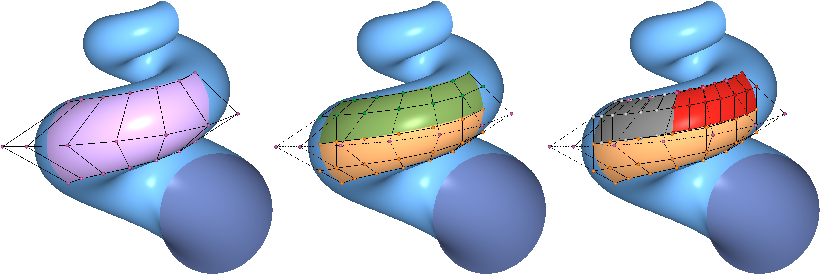
\includegraphics[width = \textwidth]{images/full_implementation_details.pdf}
		\end{flushright}
		\LinkColor{Exceptions $\bullet$ Smart pointers  $\bullet$ Cartesian, homogeneous and texture coordinates  $\bullet$  Colors, lights, materials  $\bullet$ Different template and specialized matrices $\bullet$  Constants and utility functions $\bullet$ Shader programs  $\bullet$ Generic curves and simple triangle meshes  $\bullet$  Abstract linear combinations and tensor product surfaces  $\bullet$ Characteristic polynomials, EC spaces, B-curves and B-surfaces}
	}
\end{savequote}

\chapter{Full implementation details}\label{ch:Full_implementation_details}

The entire implementation of the proposed function library is explained in the exhaustively commented listings of the current chapter.  Our library assumes that the user has a multi-core CPU and also a GPU that is compatible at least with the desktop variant of OpenGL 3.0. In order to render the geometry, we use vertex buffer objects through the OpenGL Extension Wrangler (GLEW) library and for multi-threading we rely on a C++ compiler that at least supports OpenMP 2.0. Apart from GLEW no other external dependencies are used. 

In its current state, the proposed function library consists of two main packages. The first of these is called \CBlue{\textbf{Core}} and includes data types that represent:
\begin{itemize}
    \item
    exceptions (\CBlue{Exception});
    \item
    Cartesian (\CBlue{Cartesian3}), homogeneous (\CBlue{Homogeneous3}) and texture coordinates (\CBlue{TCoordinate4});
    \item
    color components (\CBlue{Color4}), different types of lights (\CBlue{DirectionalLight}, \CBlue{PointLight}, \CBlue{Spotlight}) and materials (\CBlue{Material});
    \item
    mathematical constants, generic rectangular (\CBlue{Matrix}$<$\CPurple{T}$>$, \CBlue{RowMatrix}$<$\CPurple{T}$>$, \CBlue{Column\-Ma\-trix}$<$\break{}\CPurple{T}$>$) or triangular template matrices (\CBlue{TriangularMatrix}$<$\CPurple{T}$>$), real matrices (\CBlue{RealMatrix}: \CRed{public} \CBlue{Matrix}$<$\CRed{double}$>$), some real matrix decompositions (\CBlue{PLUDecomposition}, \CBlue{Facto\-rized\-Un\-piv\-ot\-ed\-LU\-De\-com\-po\-si\-tion}, \CBlue{SVDecomposition}), generic and derived OpenGL transformations (\CBlue{GLTransformation}, \CBlue{Translate}, \CBlue{Scale}, \CBlue{Rotate}, \CBlue{PerspectiveProjection}, \CBlue{OrthogonalProjection}, \CBlue{LookAt}) and Pascal triangles of binomial coefficients (\CBlue{PascalTriangle}: \CRed{public} \CBlue{TriangularMatrix}$<$\CRed{double}$>$);
    \item
    generic and specialized smart pointers (\CBlue{SmartPointer}$<$\CPurple{T},\CPurple{TSP},\CPurple{TOP},\CPurple{TICP},\CPurple{TCP}$>$, \CBlue{SP}$<$\CPurple{T}$>$::\CBlue{De\-faultPrimitive}, \CBlue{SP}$<$\CPurple{T}$>$::\CBlue{De\-fault}, \CBlue{SP}$<$\CPurple{T}$>$::\CBlue{Array}, \CBlue{SP}$<$\CPurple{T}$>$::\CBlue{DestructiveCopy}, \CBlue{SP}$<$\CPurple{T}$>$::\CBlue{NonIn\-tru\-siveReferenceCounting}) that provide different storage, ownership, implicit conversion and checking policies (\CBlue{StoragePolicy}$<$\CPurple{T}$>$::\CBlue{Default}, \CBlue{StoragePolicy}$<$\CPurple{T}$>$::\CBlue{Array}, \CBlue{OwnershipPolicy}$<$\break{}\CPurple{T}$>$, \CBlue{ImplicitConversionPolicy}, \CBlue{CheckingPolicy}$<$\CPurple{T}$>$::\CBlue{No\-Check}, \CBlue{CheckingPolicy}$<$\CPurple{T}$>$::\CBlue{Reject\-Null\-Deref\-er\-ence\-Or\-Indirection}, \CBlue{CheckingPolicy}$<$\CPurple{T}$>$::\CBlue{RejectNull},   \CBlue{CheckingPolicy}$<$\CPurple{T}$>$::\CBlue{As\-sert\-Null\-Deref\-er\-ence\-Or\-Indirection}, \CBlue{CheckingPolicy}$<$\CPurple{T}$>$::\CBlue{AssertNull}) in order to avoid memory leaks and to ensure exception safety (one of the most frequently used smart pointers will be the specialized variant \CBlue{SP}$<$\CPurple{T}$>$::\CBlue{Default} that ensures default storage and deep copy policies, disallows implicit conversion and rejects null dereference or indirection);
    \item
    generic curves (\CBlue{GenericCurve3}) and abstract linear combinations (\CBlue{LinearCombination3});
    \item
    triangular faces (\CBlue{TriangularFace}), simple triangle meshes (\CBlue{TriangleMesh3}) and abstract tensor product surfaces (\CBlue{TensorProductSurface3});
    \item
    shader programs\footnote{For convenience we have also provided shader programs for simple (flat) color shading, for two-sided per pixel lighting that is able to handle user-defined directional, point and spotlights with uniform front and back materials, and another one for reflection lines that are combined with two-sided per pixel lighting. All figures of the current user manual and of the paper \citep{Roth2018a} were rendered by using these shader programs. 
        %        If these would not be sufficient, more experienced users are invited to implement and use their custom shader programs and to append the provided function library with new special effects like in an open source project.
    } (\CBlue{ShaderProgram}) written in the OpenGL Shading Language and used for rendering geometries (like control polygons and nets, or generic curves and triangle meshes obtained, e.g.,\ as the images of linear combinations and tensor product surfaces, respectively).
\end{itemize}

The previously listed classes serve the definition, implementation and testing of the following data types that realize our main objectives and are included in the second main package called \CBlue{\textbf{EC}}:

\begin{itemize}
    \item
    the class \CBlue{CharacteristicPolynomial} ensures the factorization management and evaluation of characteristic polynomials of type (\ref{eq:characteristic_polynomial});
    
    \item
    EC spaces that comprise the constants and can be identified with the solution spaces of differential equations of type (\ref{eq:differential_equation}) will be instances of the class \CBlue{ECSpace};
    
    \item
    B-curves of type (\ref{eq:B_curve}) are represented by the class \CBlue{BCurve3} that is derived from the abstract base class \CBlue{LinearCombination3} and is based on the results of Corollary \ref{cor:B_basis_derivatives}, Lemma \ref{lem:general_order_elevation} and Theorems \ref{thm:general_subdivision},  \ref{thm:efficient_basis_transformation}--\ref{thm:integral_curves};
    
    \item
    B-surfaces of type (\ref{eq:B-surface}) are represented by the class \CBlue{BSurface3} that is a descendant of the abstract base class \CBlue{TensorProductSurface3} and is based on Theorem \ref{thm:integral_surfaces} and on the natural extensions of Corollary \ref{cor:B_basis_derivatives}, Lemma \ref{lem:general_order_elevation} and Theorem \ref{thm:general_subdivision}.
\end{itemize}

The tree-view of the header files that can be included from our library is illustrated in Fig.\ \mref{fig:function_library_structure} and, in what follows, we detail the implementation of each of the previously listed data types.

\begin{figure}[!h]
    \centering
    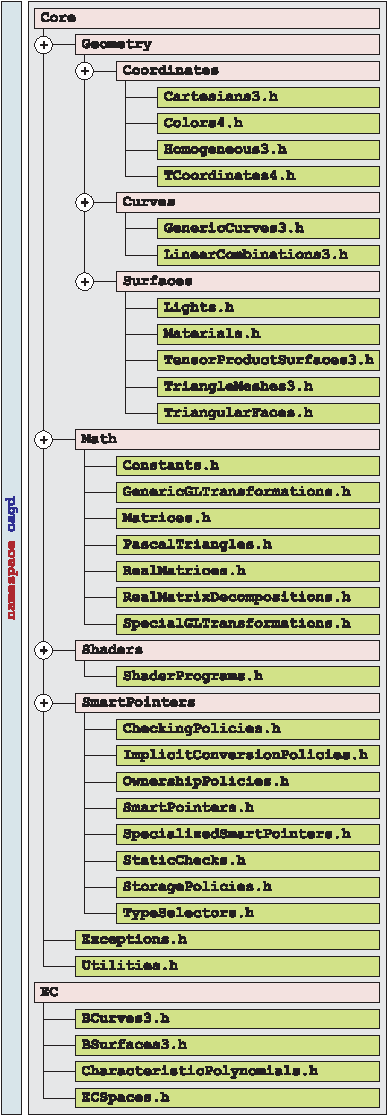
\includegraphics[scale = 1.05]{images/function_library_structure_01.pdf}
    \caption{Tree-view of the header files of the proposed function library}
    \label{fig:function_library_structure}
\end{figure}

\section{Exceptions}

We provide a simple class for possible exception handling as it is illustrated in Listing \mref{src:Exceptions.h}.

\ccode{1}{listings/Core/Exceptions.h}{src:Exceptions.h}{Exceptions (\textbf{Core/Exceptions.h})}{13}

\section{Smart pointers}
Based on \citep{Alexandrescu2001} we provide several classes to handle generic smart pointers (\CBlue{SmartPointer}) that ensure different storage, ownership, implicit conversion and checking policies in order to avoid memory leaks and to ensure exception safety. The following subsections at first detail these different policy classes, then they also define generic and specialized smart pointers by multiple inheritance.

\subsection{Type selectors}

Type selectors will be used for both enabling/disabling the implicit conversion policy and to determine the copied type in case of the storage policies.

\ccode{1}{listings/Core/SmartPointers/TypeSelectors.h}{src:TypeSelectors.h}{Type selectors (\textbf{Core/SmartPointers/TypeSelectors.h})}{15}

\subsection{Implicit conversion policies}

The class diagram of implicit conversion policies is illustrated in Fig.\ \mref{fig:UMLImplicitConversionPolicy}. Their implementation can be found in Listing \mref{src:ImplicitConversionPolicies.h}.

\begin{figure}[!h]
	\centering
	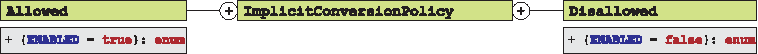
\includegraphics[]{images/UMLImplicitConversionPolicy.pdf}
	\caption{Possible implicit conversion policies ensured by our smart pointers}
	\label{fig:UMLImplicitConversionPolicy}
\end{figure}

\ccode{1}{listings/Core/SmartPointers/ImplicitConversionPolicies.h}{src:ImplicitConversionPolicies.h}{Implicit conversion policies (\textbf{Core/SmartPointers/ImplicitConversionPolicies.h})}{15}

\subsection{Static checks}

In order to include the possible compile time errors related to our smart pointers into the error list generated by the compiler, we need to provide a mechanism that performs static checks by using a macro. The definition of this macro can be found in Listing \mref{src:StaticChecks.h}.

\ccode{1}{listings/Core/SmartPointers/StaticChecks.h}{src:StaticChecks.h}{Static checks (\textbf{Core/SmartPointers/StaticChecks.h})}{15}

\subsection{Ownership policies}

Currently one can choose from the no-copy, deep copy, deep primitive copy, destructive copy and non-intrusive reference counting ownership policies. There are other (like copy-on-write, intrusive reference counting and reference linking) ownership policies as well that can be incorporated into the current implementation by following the examples provided in Listing \mref{src:OwnershipPolicies.h}.

Note that, if one applies our smart pointers with deep copy ownership policy to one of their custom types, then the corresponding class should provide a (virtual) constant cloning member function named ``clone" that returns a raw pointer to a new dynamically allocated object of the same type obtained by the invocation of the copy constructor of the class (the user is responsible for the correctness of the copy constructor). If such a custom class serves as the base of further derived classes, then the cloning function of the base should be virtual and has to be redeclared and redefined in each of the derived classes. Another possibility for the users is to derive all their custom types from the abstract base class provided in Listings \mref{src:AbstractBases.h}.

\ccode{1}{listings/Core/SmartPointers/AbstractBases.h}{src:AbstractBases.h}{Abstract base class for deep copy ownership policy in case of custom types}{1}

The class diagram of the provided ownership policies is illustrated in Fig.\ \mref{fig:UMLOwnershipPolicy}, while their implementation can be found in Listing \mref{src:OwnershipPolicies.h}. 

\begin{figure}[!h]
	\centering
	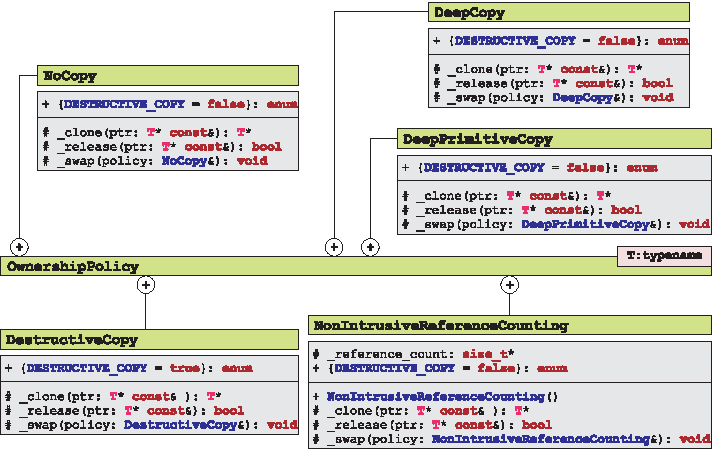
\includegraphics[]{images/UMLOwnershipPolicy.pdf}
	\caption{Possible ownership policies ensured by our smart pointers}
	\label{fig:UMLOwnershipPolicy}
\end{figure}

\newpage{}

\ccode{1}{listings/Core/SmartPointers/OwnershipPolicies.h}{src:OwnershipPolicies.h}{Ownership policies (\textbf{Core/SmartPointers/OwnershipPolicies.h})}{15}

\subsection{Storage policies}

The user can choose between the default (i.e., non-array) and array storage policies. Note that the array storage policy can only be combined with the no-copy ownership policy, since we do not know the size of the array referenced by the raw pointer that is stored in such a smart pointer. The class diagram of the aforementioned storage policies are illustrated in Fig.\ \mref{fig:UMLStoragePolicy}, while their implementations can be found in Listing \mref{src:StoragePolicies.h}. 

\begin{figure}[!h]
	\centering
	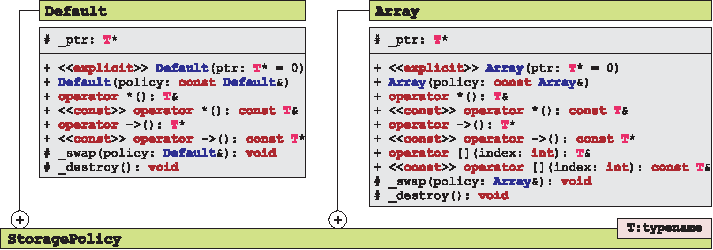
\includegraphics[]{images/UMLStoragePolicy.pdf}
	\caption{Possible storage policies ensured by our smart pointers}
	\label{fig:UMLStoragePolicy}
\end{figure}

\ccode{1}{listings/Core/SmartPointers/StoragePolicies.h}{src:StoragePolicies.h}{Storage policies (\textbf{Core/SmartPointers/StoragePolicies.h})}{15}

\subsection{Checking policies}

The user can choose from the ``reject null dereference or indirection", ``reject null", ``assert null dereference or indirection" and ``assert null" checking policies. The last two of them are based on the usage of the macro \CRed{assert}, they are invoked only under debug mode and will terminate the execution of the program. The possible checking policies are illustrated in Fig.\ \mref{fig:UMLCheckingPolicy}, while their implementations can be found in Listing \mref{src:CheckingPolicies.h}. 

\begin{figure}[!h]
	\centering
	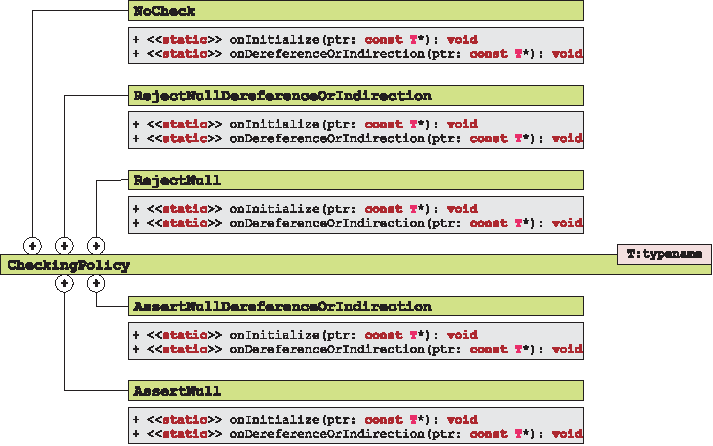
\includegraphics[]{images/UMLCheckingPolicy.pdf}
	\caption{Possible checking policies ensured by our smart pointers}
	\label{fig:UMLCheckingPolicy}
\end{figure}



\ccode{1}{listings/Core/SmartPointers/CheckingPolicies.h}{src:CheckingPolicies.h}{Checking policies (\textbf{Core/SmartPointers/CheckingPolicies.h})}{15}

\subsection{Smart pointers}

Using the implicit conversion, ownership, storage and checking policies as base classes, we define generic smart pointers by multiple inheritance as it is detailed in Listing \mref{src:SmartPointers.h}.



\ccode{1}{listings/Core/SmartPointers/SmartPointers.h}{src:SmartPointers.h}{Smart pointers (\textbf{Core/SmartPointers/SmartPointers.h})}{15}

\subsection{Frequently used specialized smart pointers}

Listing \mref{src:SpecializedSmartPointers.h} provides simpler type definitions for the most frequently used smart pointers. For example, the specialized smart pointer \CBlue{SP}$<$\CPurple{T}$>$::\CBlue{Default} ensures default storage and deep copy policies, disallows implicit conversion and rejects null dereference or indirection.
 
\ccode{1}{listings/Core/SmartPointers/SpecializedSmartPointers.h}{src:SpecializedSmartPointers.h}{Specialized smart pointers (\textbf{Core/SmartPointers/SpecializedSmartPointers.h})}{15}

\section{Cartesian coordinates}

In order to implement mathematical formulas related to B-curves/surfaces in a more natural way, we also provide a class for $3$-dimensional Cartesian coordinates (\CBlue{Cartesian3}) that ensures several useful overloaded arithmetical, logical, indexing and output/input stream operators. By means of these coordinates one can describe and store curve/surface points, higher order (mixed partial) derivatives, (unit) normal vectors associated with surface points, data that have to be interpolated, vertices of control polygons, of nets and of triangle meshes. Thus, these coordinates form the most elementary building blocks for the majority of the forthcoming classes. Fig.\ \mref{fig:UMLCartesian3} illustrates its diagram, while Listing \mref{src:Cartesians3.h} provides its implementation.

\begin{figure}[!h]
	\centering
	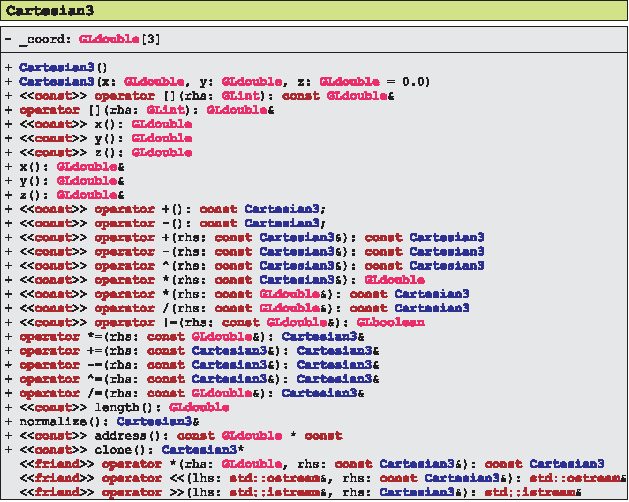
\includegraphics[]{images/UMLCartesian3.pdf}
	\caption{Class diagram of $3$-dimensional Cartesian coordinates}
	\label{fig:UMLCartesian3}
\end{figure}

\newpage{}

\ccode{1}{listings/Core/Geometry/Coordinates/Cartesians3.h}{src:Cartesians3.h}{$3$-dimensional Cartesian coordinates (\textbf{Core/Geometry/Coordinates/Cartesians3.h})}{13}

\section{Homogeneous coordinates}

Cartesian coordinates are not able to describe points at infinity. In order to overcome this problem, we will use homogeneous coordinates which are used in projective geometry and they have the advantage that the coordinates of points, including points at infinity, can be represented using finite coordinates. Formulas based on homogeneous coordinates are often simpler and more symmetric then their Cartesian counterparts. Moreover, they allow affine transformations and, in general, projective transformations to be easily represented by matrices.

Fig.\ \mref{fig:UMLHomogeneous3} illustrates the diagram, while Listing \mref{src:Homogeneous3.h} provides the implementation of the class \blue{Homogeneous3}, i.e., of $3$-dimensional homogeneous coordinates. Note, that we will mostly use this class in case of coordinate and point transformations or to define light positions and directions. Since these operations are graphics related, it is sufficiently enough to store the homogeneous coordinates in an array of single-precision floating-point values.

\begin{figure}[!h]
    \centering
    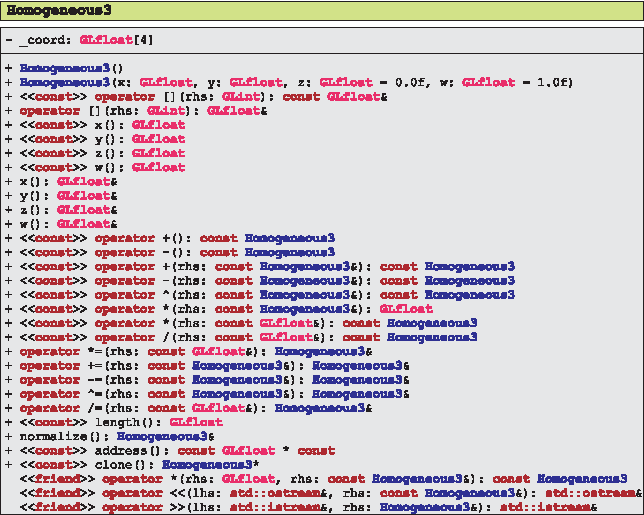
\includegraphics[]{images/UMLHomogeneous3.pdf}
    \caption{Class diagram of $3$-dimensional homogeneous coordinates}
    \label{fig:UMLHomogeneous3}
\end{figure}



\ccode{1}{listings/Core/Geometry/Coordinates/Homogeneous3.h}{src:Homogeneous3.h}{$3$-dimensional homogeneous coordinates (\textbf{Core/Geometry/Coordinates/Homogeneous3.h})}{13}

\section{Texture coordinates}

One can also handle $1$-, $2$- and $3$-dimensional and even projective texture coordinates by using the class \CBlue{TCoordinate4} whose diagram is illustrated in Fig.\ \mref{fig:UMLTCoordinate4}, while its definition and implementation can be found in Listing \mref{src:TCoordinates4.h}.

\begin{figure}[!h]
    \centering
    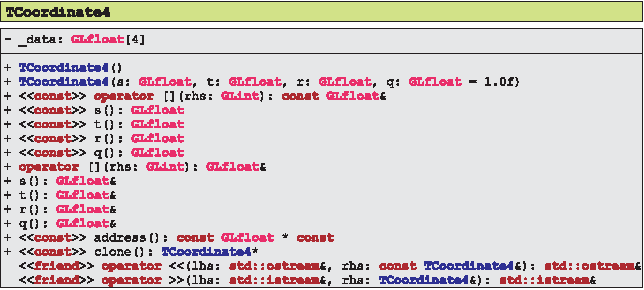
\includegraphics[]{images/UMLTCoordinate4.pdf}
    \caption{Class diagram of $1$-, $2$- and $3$-dimensional or projective texture coordinates}
    \label{fig:UMLTCoordinate4}
\end{figure}



\ccode{1}{listings/Core/Geometry/Coordinates/TCoordinates4.h}{src:TCoordinates4.h}{Texture coordinates (\textbf{Core/Geometry/Coordinates/TCoordinates4.h})}{13}

\section{Colors}

In some of our examples we will use predefined color objects that provide fixed values for red, green, blue and alpha channels. The definition and implementation of the class \CBlue{Color4} can be found in Listing \mref{src:Colors4.h}, while its diagram is presented in Fig.\ \mref{fig:UMLColor4}. Color instances can also be used to describe ambient, diffuse and specular light intensities and to define reflection coefficients in case of materials.

\begin{figure}[!h]
    \centering
    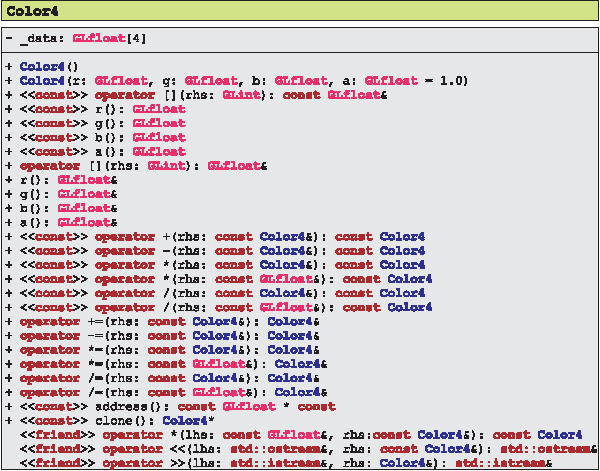
\includegraphics[]{images/UMLColor4.pdf}
    \caption{Class diagram of colors with red, green, blue and alpha channels}
    \label{fig:UMLColor4}
\end{figure}

\ccode{1}{listings/Core/Geometry/Coordinates/Colors4.h}{src:Colors4.h}{Colors (\textbf{Core/Geometry/Coordinates/Colors4.h})}{13}

\section{Lights}

We also provide data structures for directional, point and spotlights that can be used to define light instances which can be sent as uniform variables to shader programs instantiated from our class \CBlue{ShaderProgram} that is defined and implemented in Listings \mref{src:ShaderPrograms.h} and \mref{src:ShaderPrograms.cpp}, respectively. Our shader programs assume that light sources are defined by means of the structure \CBlue{LightSource} detailed in Listing \mref{src:LightSources.shader}.

\ccode{1}{listings/Core/Geometry/Surfaces/LightSources.shader}{src:LightSources.shader}{Light source data structures assumed by our shader programs}{1}

Note that in order to render the geometry and to handle different types of light objects it is not necessary to use the provided class \CBlue{ShaderProgram}. As we will see, each of our rendering methods has two overloaded variants. The first one assumes that the rendering is done through a \CBlue{ShaderProgram} instance, while the second one accepts locations of user-defined position, color, normal and (possibly projective) texture attributes of types \CRed{vec3}, \CRed{vec4}, \CRed{vec3} and \CRed{vec4}, respectively, i.e., users may define their custom shader program classes and light source objects in a totally different way. Naturally, in the latter case the handling of attributes and the communication with uniform variables are the obligations of the user. These second variants of our rendering methods will verify whether the given attribute locations can be found in the list of active attribute locations of the currently active shader program and whether they are associated with attributes of correct types.

Classes \CBlue{DirectionalLight}, \CBlue{PointLight} and \CBlue{Spotlight} were introduced in our function library for convenience in order to ease the communication with our \CBlue{ShaderProgram} instances. Their class diagrams are illustrated in Figs. \mref{fig:UMLDirectionalLight}, \mref{fig:UMLPointLight} and \mref{fig:UMLSpotlight}, while their definitions and implementations can be found in Listings \mref{src:Lights.h} and \mref{src:Lights.cpp}, respectively.

\begin{figure}[!h]
    \centering
    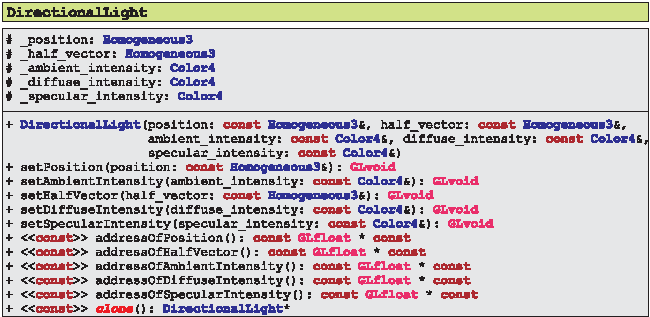
\includegraphics[]{images/UMLDirectionalLight.pdf}
    \caption{Class diagram of directional lights}
    \label{fig:UMLDirectionalLight}
\end{figure}

\begin{figure}[!h]
    \centering
    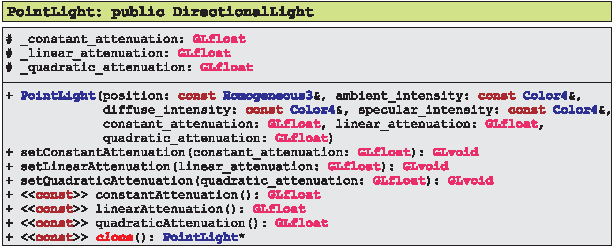
\includegraphics[]{images/UMLPointLight.pdf}
    \caption{Class diagram of point lights}
    \label{fig:UMLPointLight}
\end{figure}

\begin{figure}[!h]
    \centering
    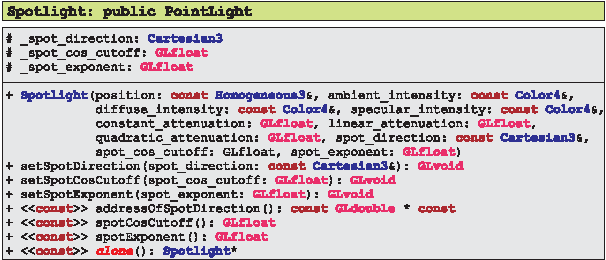
\includegraphics[]{images/UMLSpotlight.pdf}
    \caption{Class diagram of spotlights}
    \label{fig:UMLSpotlight}
\end{figure}

\ccode{1}{listings/Core/Geometry/Surfaces/Lights.h}{src:Lights.h}{Directional, point and spot lights (\textbf{Core/Geometry/Surfaces/Lights.h})}{13}

\newpage{}

\ccode{1}{listings/Core/Geometry/Surfaces/Lights.cpp}{src:Lights.cpp}{Directional, point and spot lights (\textbf{Core/Geometry/Surfaces/Lights.cpp})}{13}

\section{Materials}

We also provide a class for materials whose instances can be sent as uniform variables to shader programs instantiated from our class \CBlue{ShaderProgram} that is defined and implemented in Listings \mref{src:ShaderPrograms.h} and \mref{src:ShaderPrograms.cpp}, respectively. Our shader programs assume that uniform material variables are defined by means of the structure \CBlue{Material} detailed in Listing \mref{src:Materials.shader}.

\ccode{1}{listings/Core/Geometry/Surfaces/Materials.shader}{src:Materials.shader}{Type of uniform material variables assumed by our shader programs}{1}

Note that in order to render the geometry and to handle different types of materials it is not necessary to use the provided class \CBlue{ShaderProgram}. As we will see, each of our rendering methods has two overloaded variants. The first one assumes that the rendering is done through a \CBlue{ShaderProgram} instance, while the second one accepts locations of user-defined position, color, normal and (possibly projective) texture attributes of types \CRed{vec3}, \CRed{vec4}, \CRed{vec3} and \CRed{vec4}, respectively, i.e., users may define their custom shader program classes and materials in a totally different way. Naturally, in the latter case the handling of attributes and the communication with uniform variables are the obligations of the user. These second variants of our rendering methods will verify whether the given attribute locations can be found in the list of active attribute locations of the currently active shader program and whether they are associated with attributes of correct types.

The class \CBlue{Material} was introduced in our function library for convenience in order to ease the communication with our \CBlue{ShaderProgram} instances, its diagram is illustrated in Fig.\ \mref{fig:UMLMaterial}, while its definition and implementation can be found in Listings \mref{src:Materials.h} and \mref{src:Materials.cpp}, respectively. We also provide in lines \mref{src:predefined_materials:start}--\mref{src:predefined_materials:end} of Listing \mref{src:Materials.cpp} predefined materials like black plastique, black rubber, brass, bronze, chrome, copper, emerald, gold, jade, obsidian, pearl, pewter, polished bronze, polished copper, polished gold, polished silver, ruby, silver and turquoise.

\begin{figure}[!h]
    \centering
    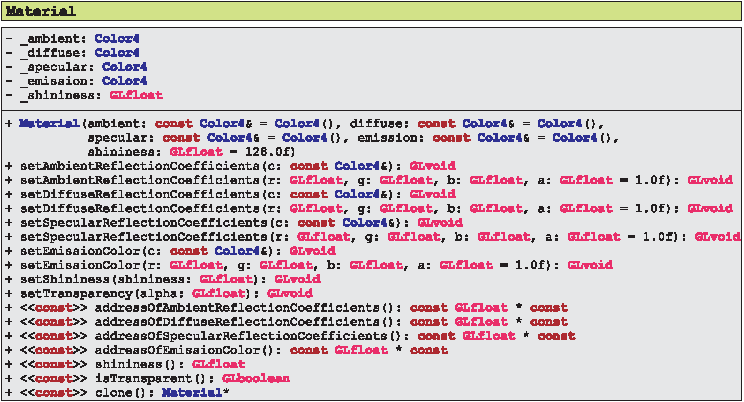
\includegraphics[]{images/UMLMaterial.pdf}
    \caption{Class diagram of materials}
    \label{fig:UMLMaterial}
\end{figure}

\ccode{1}{listings/Core/Geometry/Surfaces/Materials.h}{src:Materials.h}{Materials (\textbf{Core/Geometry/Surfaces/Materials.h})}{13}

\ccode{1}{listings/Core/Geometry/Surfaces/Materials.cpp}{src:Materials.cpp}{Materials (\textbf{Core/Geometry/Surfaces/Materials.cpp})}{13}


\section{Different template and specialized matrices}

\subsection{Generic template matrices}

In order to  represent traditional matrices, knot and weight vectors, control polygons and nets, Pascal triangles of binomial coefficients, triangle matrices of partial derivatives, or data point sequences and grids that have to be interpolated, we also define rectangular, column, row and triangular template matrices (\CBlue{Matrix}$<$\CPurple{T}$>$, \CBlue{ColumnMatrix}$<$\CPurple{T}$>$, \CBlue{RowMatrix}$<$\CPurple{T}$>$ and \CBlue{TriangularMatrix}$<$\CPurple{T}$>$). Fig.\ \mref{fig:UMLTemplateMatrices} illustrates the diagrams of these classes. Their implementation can be found in Listing \mref{src:Matrices.h}.

\begin{figure}[!h]
	%		\vspace{-3\baselineskip}
	\centering
	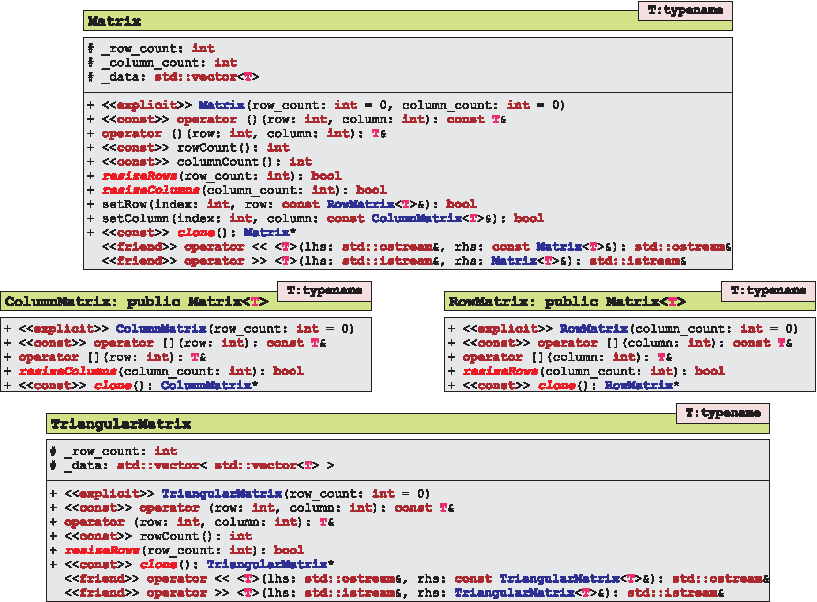
\includegraphics[]{images/UMLTemplateMatrices+.pdf}
	\caption{Class diagrams of different types of template matrices}
	\label{fig:UMLTemplateMatrices}
\end{figure}

\ccode{1}{listings/Core/Math/Matrices.h}{src:Matrices.h}{Rectangular, row, column and triangular template matrices (\textbf{Core/Math/Matrices.h})}{13}

Triangular matrices will be used to store either all (mixed) partial derivatives of a smooth surface up to a specified maximum order of differentiation, or Pascal triangles of binomial coefficients that are required for the evaluation of differentiation formulas which are based on the application of the Leibniz rule. The definition and implementation of Pascal triangles can be found in Listings \mref{src:PascalTriangles.h} and \mref{src:PascalTriangles.cpp}, respectively.

\ccode{1}{listings/Core/Math/PascalTriangles.h}{src:PascalTriangles.h}{Pascal triangles of binomial coefficients (\textbf{Core/Math/PascalTriangles.h})}{13}

\ccode{1}{listings/Core/Math/PascalTriangles.cpp}{src:PascalTriangles.cpp}{Pascal triangles of binomial coefficients (\textbf{Core/Math/PascalTriangles.cpp})}{13}

\subsection{Real matrices and decompositions}

We also provide real matrices (\CBlue{RealMatrix}:\ \CRed{public} \CBlue{Matrix}$<$\CRed{double}$>$) and data structures (like \CBlue{PLUDecomposition}, \CBlue{Factorized\-Un\-piv\-o\-ted\-LU\-Decomposition} and \CBlue{SVDecomposition}) for pivoted and non-pivoted Doolittle-type $LU$ decompositions and for singular value decompositions as well.

Real matrices provide multi-threaded arithmetical operators for matrix related operations, while using different matrix decompositions we are able:
\begin{itemize}
    \item to solve by multi-threading linear systems of equations described by template matrices that may appear not only in traditional real cases, but in case of curve and surface interpolation problems as well;
    
    \item to study the condition numbers of possibly ill-conditioned systems of linear of equations;
    
    \item to construct the normalized B-basis of the underlying EC spaces.
\end{itemize}

\subsubsection{Real matrices}

Diagrams of the class \CBlue{RealMatrix} and of some auxiliary real row and column matrix related arithmetical binary operators are illustrated in Fig.\ \mref{fig:UMLRealMatrix}, while their definitions and implementations can  be found in Listings \mref{src:RealMatrices.h} and \mref{src:RealMatrices.cpp}, respectively.

\begin{figure}[!h]
    \centering
    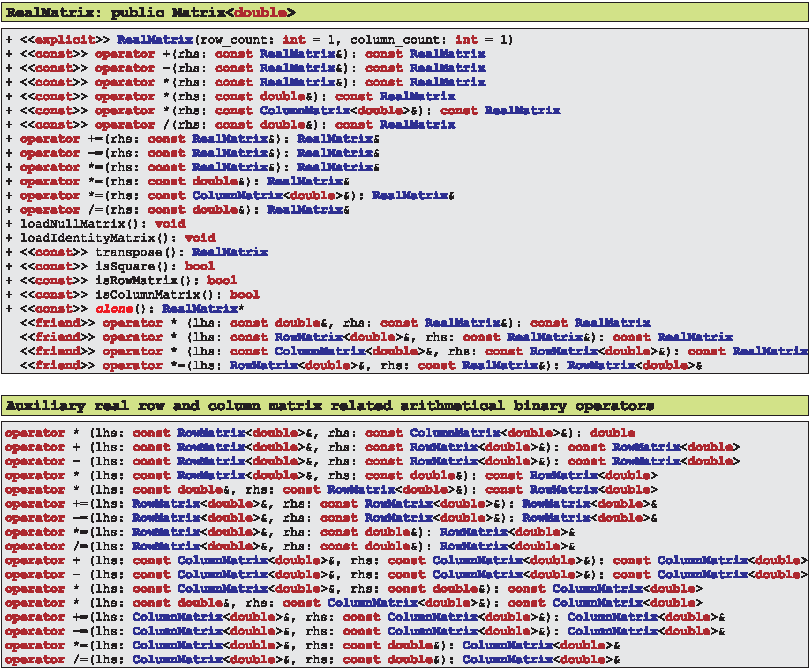
\includegraphics[]{images/UMLRealMatrix.pdf}
    \caption{Diagrams of real matrices and of some auxiliary real row and column matrix related arithmetical binary operators}
    \label{fig:UMLRealMatrix}
\end{figure} 

\ccodeNUV{1}{listings/Core/Math/RealMatrices.h}{src:RealMatrices.h}{Real matrices (\textbf{Core/Math/RealMatrices.h})}{13}

\ccodeNUV{1}{listings/Core/Math/RealMatrices.cpp}{src:RealMatrices.cpp}{Real matrices (\textbf{Core/Math/RealMatrices.cpp})}{13}

\subsubsection{$LU$ and singular value decompositions}

%The structures of these classes are illustrated in Figs.\ \mref{fig:UMLRealMatrix}, \mref{fig:PLUDecomposition},  \mref{fig:FactorizedUnpivotedLUDecomposition} and \mref{fig:SVDecomposition}.
%
%TO DO: FIGURES

Diagrams of classes \CBlue{PLUDecomposition}, \CBlue{Factorized\-Unpivoted\-LU\-De\-com\-position} and \CBlue{SVDecomposition}) are illustrated in Fig.\ \mref{fig:UMLRealMatrixDecompositions}, while their declarations and implementations can be found in Listings \mref{src:RealMatrixDecompositions.h} and \mref{src:RealMatrixDecompositions.cpp}, respectively. These parts of the proposed function library are based on \citep{PressTeukolskyVetterlingFlannery2007}.

\begin{figure}[!h]
    \centering
    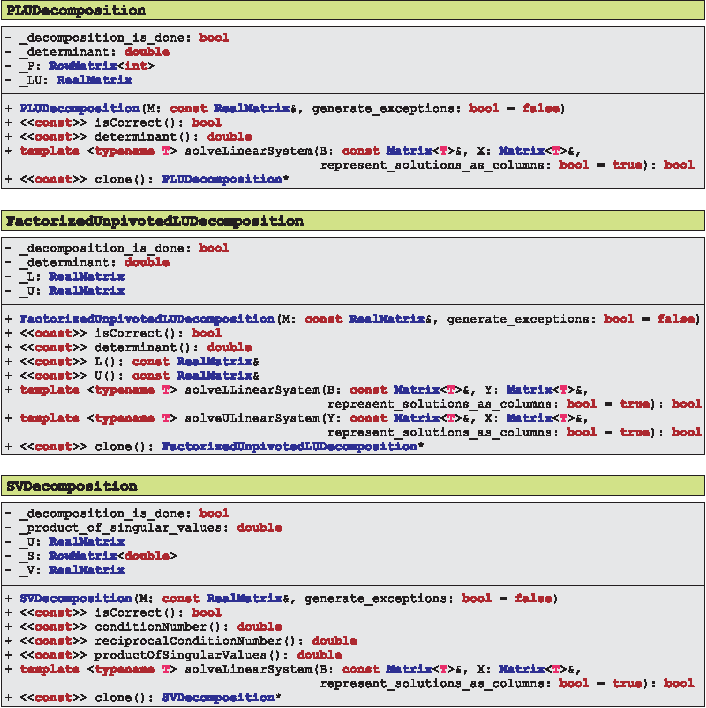
\includegraphics[]{images/UMLRealMatrixDecompositions.pdf}
    \caption{Diagrams of used real matrix decompositions}
    \label{fig:UMLRealMatrixDecompositions}
\end{figure}

\ccode{1}{listings/Core/Math/RealMatrixDecompositions.h}{src:RealMatrixDecompositions.h}{Real matrix decompositions (\textbf{Core/Math/RealMatrixDecompositions.h})}{16}

\ccode{1}{listings/Core/Math/RealMatrixDecompositions.cpp}{src:RealMatrixDecompositions.cpp}{Real matrix decompositions (\textbf{Core/Math/RealMatrixDecompositions.cpp})}{16}

\subsection{Generic and special OpenGL transformation matrices}
Since the classic OpenGL transformation commands (like \CPurple{glMultMatrix\{f$|$d\}},  \CPurple{glRotate\{f$|$d\}},  \CPurple{gl\-Trans\-late\{f$|$d\}},  \CPurple{glScale\{f$|$d\}}, \CPurple{glOrtho\{f$|$d\}},  \CPurple{gluPerspective}, \CPurple{gluLook\-At\{f$|$d\}}) and the traditional matrix stacks that are associated with the projection and model-view matrix modes are considered deprecated, we also provide classes for generic and special OpenGL transformation matrices by means of which one can define general, rotation, translation, scaling, orthogonal or perspective projection and world coordinate transformation matrices. By design, each special OpenGL transformation is derived from the generic one \CBlue{GLTransformation} that stores a $4\times 4$ column-major ordered matrix in a memory-continuous \CRed{float} array whose constant address can be sent either to our or to user-defined custom shader program objects in order to initialize/communicate with matrices defined as uniform variables of type \CRed{mat4}. The class \CBlue{GLTransformation} also defines several multi-threaded mathematical operators and auxiliary methods by means of which one can either compose more complex transformations or to transform \CBlue{Homogeneous3} and \CBlue{Cartesian3} coordinates as well. (Since matrix classes \CBlue{Matrix}$<$\CPurple{T}$>$, \CBlue{RealMatrix}:\ \CRed{public} \CBlue{Matrix}$<$\CRed{double}$>$ and \CBlue{RealSquareMatrix}:\ \CRed{public} \CBlue{RealMatrix} store their data in row-major order and OpenGL expects the transformation matrices by default in column-major order, the class \CBlue{GLTransformation} is not inherited from the matrix classes presented so far.)

The structure of the base class \CBlue{GLTransformation} is illustrated in Fig.\ \mref{fig:UMLGLTransformation}, while its definition and implementation can be found in  Listings \mref{src:GenericGLTransformations.h} and \mref{src:GenericGLTransformations.cpp}, respectively.

\begin{figure}[!h]
    \centering
    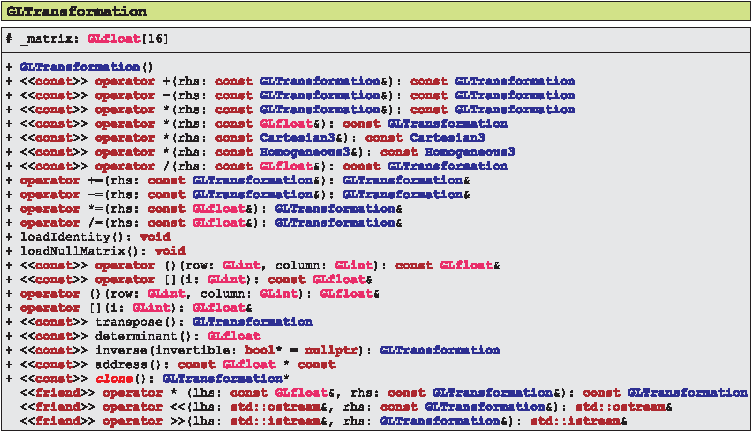
\includegraphics[]{images/UMLGLTransformation.pdf}
    \caption{Diagram of generic OpenGL transformations}
    \label{fig:UMLGLTransformation}
\end{figure}

\ccodeNUV{1}{listings/Core/Math/GenericGLTransformations.h}{src:GenericGLTransformations.h}{Generic OpenGL transformations (\textbf{Core/Math/GenericGLTransformations.h})}{13}


\ccodeNUV{1}{listings/Core/Math/GenericGLTransformations.cpp}{src:GenericGLTransformations.cpp}{Generic OpenGL transformations (\textbf{Core/Math/GenericGLTransformations.cpp})}{13}

Structures of the derived transformation matrices \CBlue{Translate}, \CBlue{Scale}, \CBlue{Rotate}, \CBlue{PerspectiveProjection}, \CBlue{OrthogonalProjection} and \CBlue{LookAt} are illustrated in Fig.\ \mref{fig:UMLSpecialGLTransformations}, while their definitions and implementations are presented in Listings \mref{src:SpecialGLTransformations.h} and \mref{src:SpecialGLTransformations.cpp}, respectively.

\begin{figure}[!h]
    \centering
    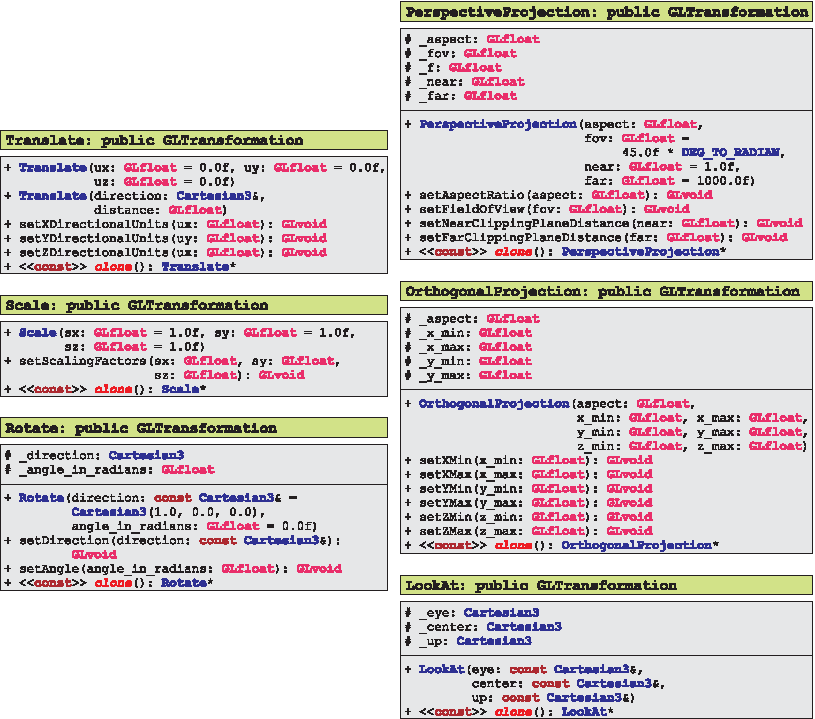
\includegraphics[]{images/UMLSpecialGLTransformations.pdf}
    \caption{Diagrams of special OpenGL transformations}
    \label{fig:UMLSpecialGLTransformations}
\end{figure}

\ccodeNUV{1}{listings/Core/Math/SpecialGLTransformations.h}{src:SpecialGLTransformations.h}{Special OpenGL transformations (\textbf{Core/Math/SpecialGLTransformations.h})}{13}

\newpage

\ccodeNUV{1}{listings/Core/Math/SpecialGLTransformations.cpp}{src:SpecialGLTransformations.cpp}{Special OpenGL transformations (\textbf{Core/Math/SpecialGLTransformations.cpp})}{13}

\section{Constants and utility functions}

Using some of the classes detailed so far, we also provide some frequently used constants and utility functions in Listings \mref{src:Constants.h} and \mref{src:Utilities.h}/\mref{src:Utilities.cpp}, respectively.

\ccodeNUV{1}{listings/Core/Math/Constants.h}{src:Constants.h}{Constants (\textbf{Core/Math/Constants.h})}{13}

\ccode{1}{listings/Core/Utilities.h}{src:Utilities.h}{Utility functions (\textbf{Core/Utilities.h})}{13}

\ccodeNUV{1}{listings/Core/Utilities.cpp}{src:Utilities.cpp}{Utility functions (\textbf{Core/Utilities.cpp})}{13}

\section{Shader programs}

In order to render geometries (like control polygons and nets, or generic curves and triangle meshes obtained, e.g.,\ as the images of linear combinations and tensor product surfaces, respectively), we rely on shader programs written in the OpenGL Shading Language. As we will present later on, classes \CBlue{Generic\-Curve3}, \CBlue{TriangleMesh3}, \CBlue{BCurve3}:\ \CRed{public} \CBlue{LinearCombination3} and \CBlue{BSurface3}:\ \CRed{public} \CBlue{TensorProductSurface3} provide several rendering methods. Each of them have two variants, the first of these overloaded member functions relies on instances of our class \CBlue{ShaderProgram} detailed in Listings \mref{src:ShaderPrograms.h} and \mref{src:ShaderPrograms.cpp} below, while the second one assumes that users handle their shader programs in a different way by providing at the same time attribute (like position, color, normal and texture coordinate) locations of proper types as input parameters for this second variant of our rendering methods. The latter variants will return a false value whenever one of the followings happens: the users did not activate their custom shader programs; the given attribute locations cannot be found in the list of active attribute locations, or they exist but are associated with attributes that have incorrect types (positions, colors, normals and texture coordinate attribute variables have to be of types \CRed{vec3}, \CRed{vec4}, \CRed{vec3} and \CRed{vec4}, respectively); the rendering mode or other input parameters are invalid. For more details on the input and output parameters of our rendering methods consider later the lines \mref{src:GenericCurve3:renderDerivatives:start}--\mref{src:GenericCurve3:renderDerivatives:end}, \mref{src:TrinagleMesh3:render:start}--\mref{src:TrinagleMesh3:render:end},  \mref{src:LinearCombination3:renderData:start}--\mref{src:LinearCombination3:renderData:end} and \mref{src:TensorProductSurface3:render:start}--\mref{src:TensorProductSurface3:render:end} of Listings \mref{src:GenericCurves3.h}, \mref{src:TriangleMeshes3.h},  \mref{src:LinearCombinations3.h} and \mref{src:TensorProductSurfaces3.h}, respectively. 

Section \mref{sec:Using_our_shader_programs} provides examples for the usage of our class \CBlue{ShaderProgram} and for convenience also describes shader programs for simple (flat) color shading, for two-sided per pixel lighting (that is able to handle user-defined directional, point and spotlights with uniform front and back materials) and another one for reflection lines that are combined with two-sided per pixel lighting. All figures of this user manual were rendered by using these shader programs.

\ccode{1}{listings/Core/Shaders/ShaderPrograms.h}{src:ShaderPrograms.h}{Shader programs (\textbf{Core/Shaders/ShaderPrograms.h})}{13}

\ccode{1}{listings/Core/Shaders/ShaderPrograms.cpp}{src:ShaderPrograms.cpp}{Shader programs (\textbf{Core/Shaders/ShaderPrograms.cpp})}{13}

\section{Generic curves}

In order to store in vertex buffer objects the points and higher order derivatives of arbitrary smooth parametric (basis) functions, (B-)curves and isoparametric lines of (B-)surfaces, we introduce a class for generic curves (\CBlue{GenericCurve3}) that will be used for rendering purposes. Its diagram is illustrated in Fig.\ \mref{fig:UMLGenericCurve3}. Apart from vertex buffer object handling methods and some simple accessors, the class also provides overloaded function operators that can be used for reading or writing the derivatives associated with a curve point. Moreover, the class also provides a method by means of which one can generate Matlab source codes to plot the curve points and to create scalable vector graphic formats (like EPS). The declaration and implementation of the class can be found in Listings \mref{src:GenericCurves3.h} and \mref{src:GenericCurves3.cpp}, respectively.

\begin{figure}[!h]
	
	\centering
	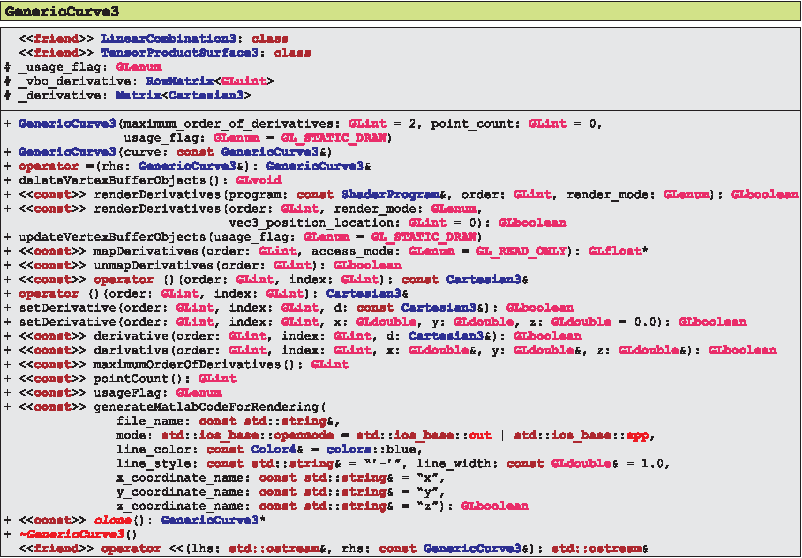
\includegraphics[]{images/UMLGenericCurve3.pdf}
	\caption{Class diagram of generic curves}
	\label{fig:UMLGenericCurve3}
\end{figure}

\ccode{1}{listings/Core/Geometry/Curves/GenericCurves3.h}{src:GenericCurves3.h}{$3$-dimensional generic curves (\textbf{Core/Geometry/Curves/GenericCurves3.h})}{13}

\ccode{1}{listings/Core/Geometry/Curves/GenericCurves3.cpp}{src:GenericCurves3.cpp}{$3$-dimensional generic curves (\textbf{Core/Geometry/Curves/GenericCurves3.cpp})}{13}

\section{Simple triangle meshes}

We also provide classes for triangular faces (\CBlue{TriangularFace}) and simple triangle meshes (\CBlue{TriangleMesh3}), by means of which one can store in vertex buffer objects the attributes (i.e., position, normal and texture coordinates, color components and connectivity information) of vertices that form the triangular faces of the mesh. 

The diagram of the class \CBlue{TriangularFace} is shown in Fig.\  \mref{fig:UMLTriangularFace}, while both of its definition and implementation can be found in Listing \mref{src:TriangularFaces.h}.

\begin{figure}[!h]
    \centering
    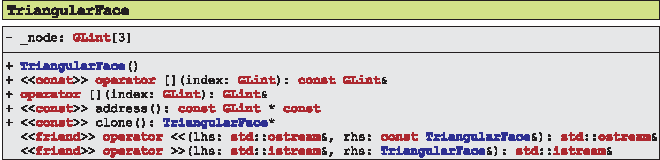
\includegraphics[]{images/UMLTriangularFace.pdf}
    \caption{Class diagram of triangular faces}
    \label{fig:UMLTriangularFace}
\end{figure}

%\newpage{}

\ccode{1}{listings/Core/Geometry/Surfaces/TriangularFaces.h}{src:TriangularFaces.h}{Triangular faces (\textbf{Core/Geometry/Surfaces/TriangularFaces.h})}{13}

The diagram of the class \CBlue{TriangleMesh3} is illustrated in Fig.\  \mref{fig:UMLTriangleMesh3}, while its definition and implementation can be found in Listings \mref{src:TriangleMeshes3.h} and \mref{src:TriangleMeshes3.cpp}, respectively.

\begin{figure}[!h]
    \centering
    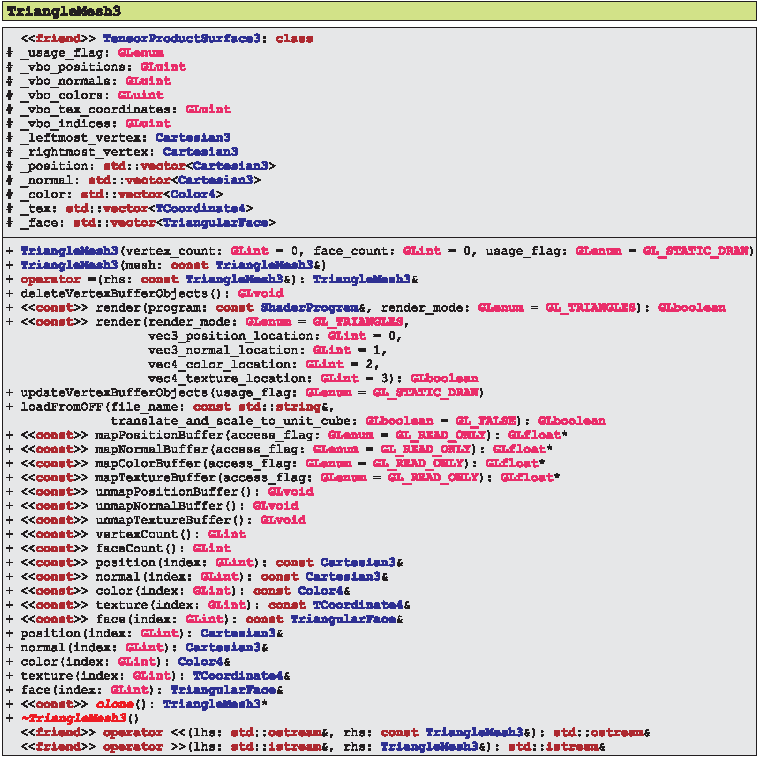
\includegraphics[]{images/UMLTriangleMesh3+.pdf}
    \caption{Class diagram of simple triangle meshes}
    \label{fig:UMLTriangleMesh3}
\end{figure}



%\vspace{-5mm}


\ccode{1}{listings/Core/Geometry/Surfaces/TriangleMeshes3.h}{src:TriangleMeshes3.h}{Simple triangle meshes (\textbf{Core/Geometry/Surfaces/TriangleMeshes3.h})}{13}

\ccode{1}{listings/Core/Geometry/Surfaces/TriangleMeshes3.cpp}{src:TriangleMeshes3.cpp}{Simple triangle meshes (\textbf{Core/Geometry/Surfaces/TriangleMeshes3.cpp})}{13}

\section[Abstract linear combinations and tensor product surfaces]{Abstract linear combinations and tensor product surfaces}

We also ensure abstract base classes for arbitrary linear combinations (\CBlue{LinearCombination3}) and tensor product surfaces (\CBlue{TensorProductSurface3}) that are able to generate their images, to update and render their control polygons or nets and to solve curve or surface interpolation problems -- provided that the user redeclares and defines in derived classes those pure virtual methods that appear in the interfaces of these abstract classes and are responsible for the evaluation of blending functions and of (partial) derivatives up to a specified maximum order of differentiation. 

Pure virtual methods that have to bo redeclared and defined in derived classes are:
\begin{itemize}
	\item 
	\CBlue{LinearCombination3}::\CDRPurple{\textit{\textbf{blendingFunctionValues}}};
	\item
	\CBlue{LinearCombination3}::\CDRPurple{\textit{\textbf{calculateDerivatives}}};
	\item
	\CBlue{TensorProductSurface3}::\CDRPurple{\textit{\textbf{blendingFunctionValues}}};
	\item
	\CBlue{TensorProductSurface3}::\CDRPurple{\textit{\textbf{calculateAllPartialDerivatives}}}; and
	\item
	\CBlue{TensorProductSurface3}::\CDRPurple{\textit{\textbf{calculateDirectionalDerivatives}}}.
\end{itemize}

As we will see in Listings \mref{src:BCurves3.h} and \mref{src:BSurfaces3.h}, B-curves and B-surfaces of type (\mref{eq:B_curve}) and (\mref{eq:B-surface}) will be derived from classes \CBlue{LinearCombination3} and \CBlue{TensorProductSurface3}, respectively.

The diagram of the abstract class \CBlue{LinearCombination3} is illustrated in Fig.\ \mref{fig:UMLLinearCombination3}, while its definition and implementation can be found in Listings \mref{src:LinearCombinations3.h} and \mref{src:LinearCombinations3.cpp}, respectively.

\begin{figure}[!htb]
	\centering
	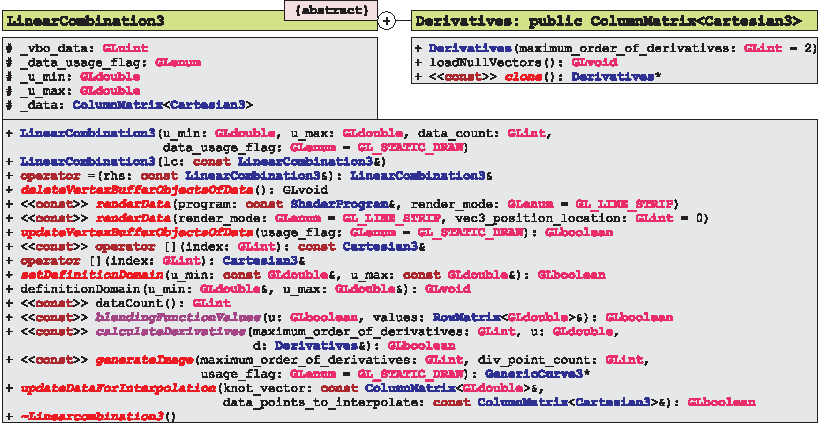
\includegraphics[]{images/UMLLinearCombination3.pdf}
	\caption{Class diagram of abstract linear combinations}
	\label{fig:UMLLinearCombination3}
\end{figure}

\ccode{1}{listings/Core/Geometry/Curves/LinearCombinations3.h}{src:LinearCombinations3.h}{Abstract linear combinations (\textbf{Core/Geometry/Curves/LinearCombinations3.h})}{13}

\ccode{1}{listings/Core/Geometry/Curves/LinearCombinations3.cpp}{src:LinearCombinations3.cpp}{Abstract linear combinations (\textbf{Core/Geometry/Curves/LinearCombinations3.cpp})}{13}

The diagram of the abstract class \CBlue{TensorProductSurface3} is illustrated in Fig.\ \mref{fig:UMLTensorProductSurface3}, while its definition and implementation can be found in Listings \mref{src:TensorProductSurfaces3.h} and \mref{src:TensorProductSurfaces3.cpp}, respectively.

\begin{figure}[!h]
	
	\centering
	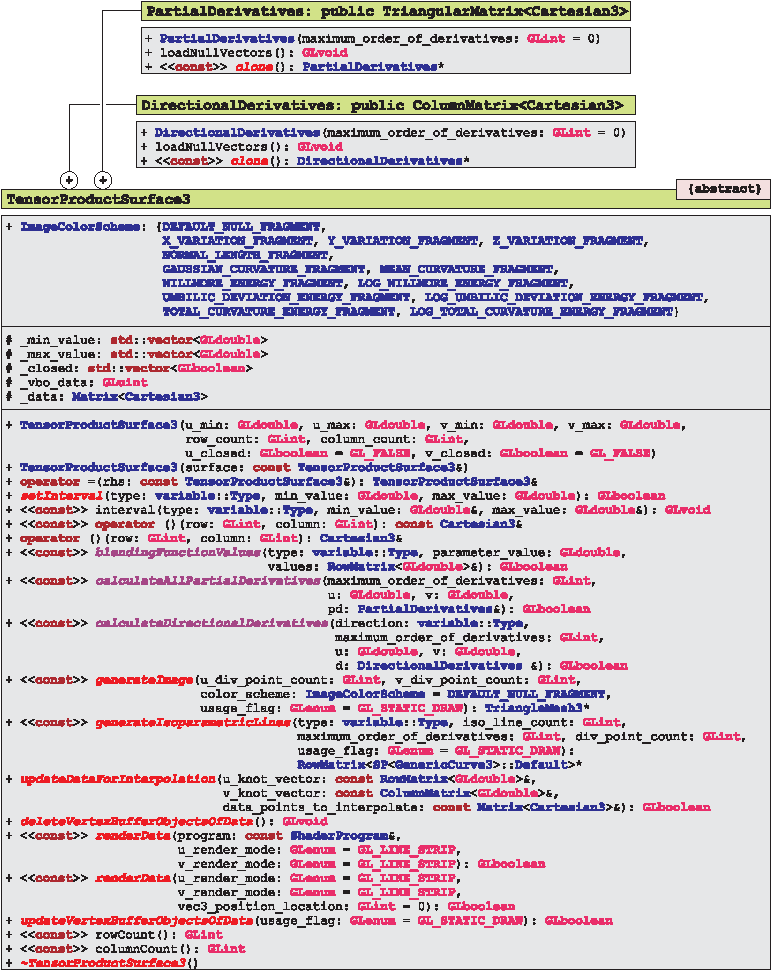
\includegraphics[]{images/UMLTensorProductSurface3.pdf}
	\caption{Class diagram of abstract tensor product surfaces}
	\label{fig:UMLTensorProductSurface3}
\end{figure}

\ccode{1}{listings/Core/Geometry/Surfaces/TensorProductSurfaces3.h}{src:TensorProductSurfaces3.h}{Abstract tensor product surfaces (\textbf{Core/Geometry/Surfaces/TensorProductSurfaces3.h})}{13}


\ccodeNUV{1}{listings/Core/Geometry/Surfaces/TensorProductSurfaces3.cpp}{src:TensorProductSurfaces3.cpp}{Abstract tensor product surfaces (\textbf{Core/Geometry/Surfaces/TensorProductSurfaces3.cpp})}{13}

\section{Characteristic polynomials}

Characteristic polynomials of type (\mref{eq:characteristic_polynomial}) will be instances of the class \CBlue{CharacteristicPolynomial} that is able to store and update the factorization of (\mref{eq:characteristic_polynomial}) and also provides an overloaded function operator for evaluation purposes. The diagram of the class is illustrated in Fig.\ \mref{fig:UMLCharacteristicPolynomial}, while its definition and implementation can be found in Listings \mref{src:CharacteristicPolynomials.h} and \mref{src:CharacteristicPolynomials.cpp}, respectively.

\begin{figure}[!h]
	
	\centering
	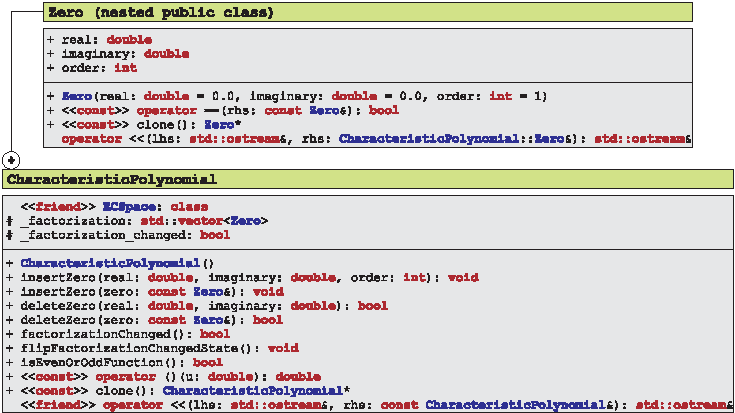
\includegraphics[]{images/UMLCharacteristicPolynomial.pdf}
	\caption{Class diagrams of characteristic polynomials and of their (higher order) zeros}
	\label{fig:UMLCharacteristicPolynomial}
\end{figure}

\ccode{1}{listings/EC/CharacteristicPolynomials.h}{src:CharacteristicPolynomials.h}{Characteristic polynomials (\textbf{EC/CharacteristicPolynomials.h})}{13}

\ccode{1}{listings/EC/CharacteristicPolynomials.cpp}{src:CharacteristicPolynomials.cpp}{Characteristic polynomials (\textbf{EC/CharacteristicPolynomials.cpp})}{13}

\section{EC spaces}
EC spaces (that comprise the constants and can be identified with the solution spaces of differential equations of type (\mref{eq:differential_equation}) defined on intervals for which the corresponding spaces of derivatives are also EC) will be instances of the class \CBlue{ECSpace} that:
\begin{itemize}
\item
is able to generate and to update both the ordinary basis and the normalized B-basis of an EC vector space specified by the factorization of a characteristic polynomial of type (\mref{eq:characteristic_polynomial});
\item
provides a function operator to evaluate the zeroth and higher order derivatives of both bases at any point of the definition domain;
\item
can also be used to generate the general basis transformation matrix formulated in Theorem \mref{thm:efficient_basis_transformation} that maps the normalized B-basis to the ordinary basis of the underlying EC space;
\item
is able to decide whether the specified EC vector is reflection invariant; 
\item
can list the \LaTeX{} expressions of the ordinary basis functions; 
\item
can also be used to generate the images of both the ordinary basis and the normalized B-basis functions.
\end{itemize}
The diagram of the class is illustrated in Fig.\ \mref{fig:UMLECSpace}, while its definition and implementation can be found in Listings \mref{src:ECSpaces.h} and \mref{src:ECSpaces.cpp}, respectively.

\begin{figure}[!h]
	
	\centering
	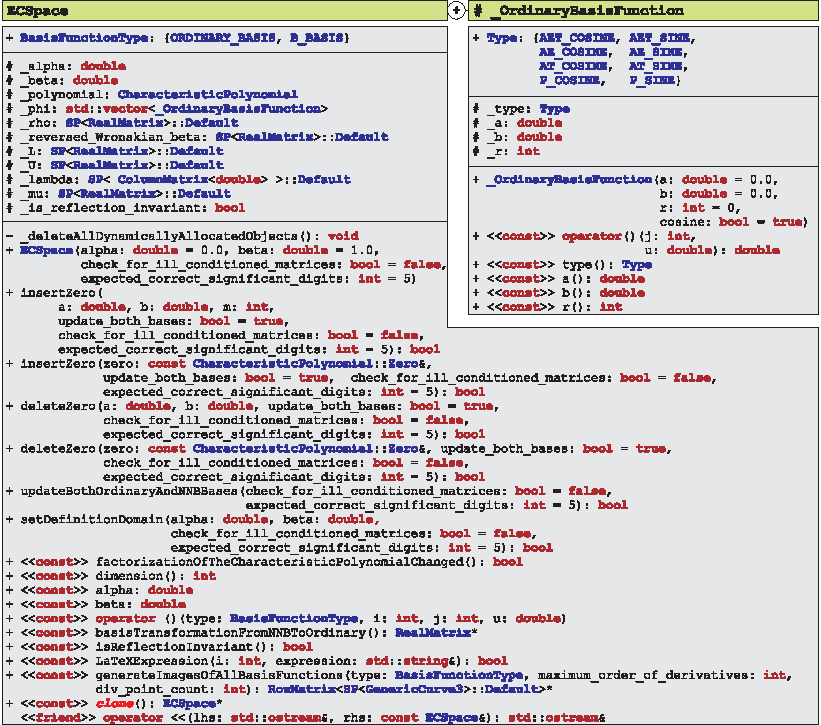
\includegraphics[]{images/UMLECSpace.pdf}
	\caption{Class diagram of constant-comprising translation invariant EC spaces that can be identified with the solution spaces of constant-coefficient homogeneous linear differential equations defined on intervals for which the corresponding spaces of derivatives are also EC}
	\label{fig:UMLECSpace}
\end{figure}

\ccode{1}{listings/EC/ECSpaces.h}{src:ECSpaces.h}{EC spaces (\textbf{EC/ECSpaces.h})}{13}

\ccodeNUV{1}{listings/EC/ECSpaces.cpp}{src:ECSpaces.cpp}{EC spaces (\textbf{EC/ECSpaces.cpp})}{13}

\section{B-curves}

B-curves of type (\mref{eq:B_curve}) are represented by the class \CBlue{BCurve3} that is derived from the abstract base class \CBlue{LinearCombination3} and is based on the results of Corollary \ref{cor:B_basis_derivatives}, Lemma \ref{lem:general_order_elevation} and Theorems \ref{thm:general_subdivision},  \ref{thm:efficient_basis_transformation}--\ref{thm:integral_curves}. It can be used to perform general order elevation, subdivision and to describe exactly user-specified ordinary integral curves by means of convex combinations of control points and normalized B-basis functions. The diagram of the class is illustrated in Fig.\ \mref{fig:UMLBCurve3}, its definition and implementation are listed in Listings \mref{src:BCurves3.h} and \mref{src:BCurves3.cpp}, respectively. Note that the class redeclares and defines those pure virtual methods that are inherited as interfaces from the abstract base class \CBlue{LinearCombination3}.

\begin{figure}[!h]
	\centering
	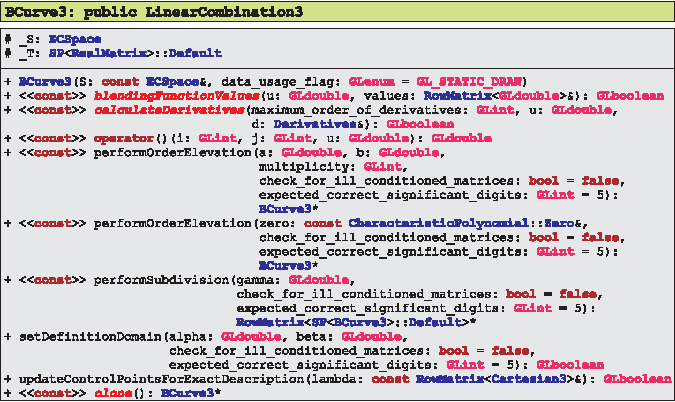
\includegraphics[]{images/UMLBCurve3.pdf}
	\caption{Class diagram of general B-curves}
	\label{fig:UMLBCurve3}
\end{figure}

\ccode{1}{listings/EC/BCurves3.h}{src:BCurves3.h}{B-curves (\textbf{EC/BCurves3.h})}{13}

\newpage

\ccode{1}{listings/EC/BCurves3.cpp}{src:BCurves3.cpp}{B-curves (\textbf{EC/BCurves3.cpp})}{13}

\section{B-surfaces}

B-surfaces of type (\mref{eq:B-surface}) are represented by the class \CBlue{BSurface3} that is derived from the abstract base class \CBlue{TensorProductSurface3}. It is based on Theorem \mref{thm:integral_surfaces} and on the natural extensions of Corollary \mref{cor:B_basis_derivatives}, Lemma \mref{lem:general_order_elevation} and Theorem \mref{thm:general_subdivision}. It can be used to perform general order elevation, subdivision and to describe exactly a large family of ordinary integral surfaces of type (\mref{eq:ordinary_integral_surface}). Its diagram is presented in Fig.\ \mref{fig:UMLBSurface3}, while its definition and implementation can be found in Listings \mref{src:BSurfaces3.h} and \mref{src:BSurfaces3.cpp}. Note that the class redeclares and defines those pure virtual methods that are inherited from the abstract base class \CBlue{TensorProductSurface3}.

\begin{figure}[!h]
	
	\centering
	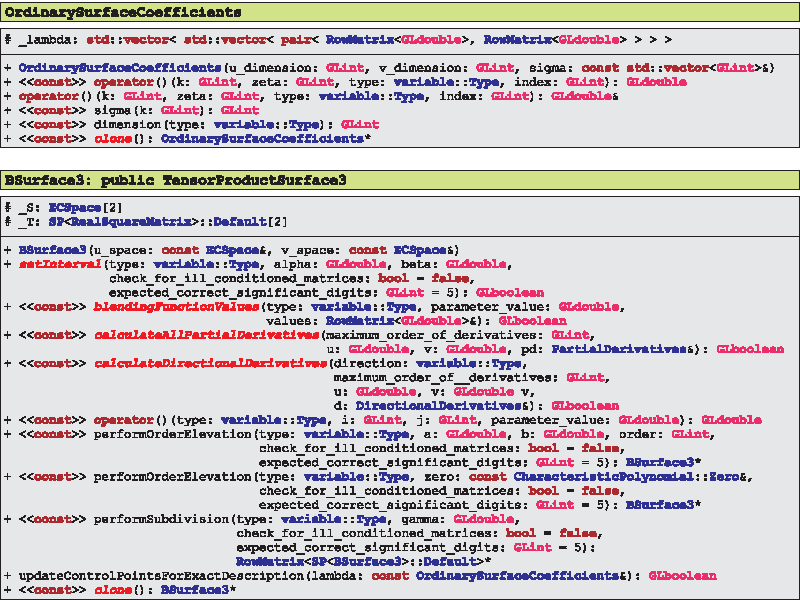
\includegraphics[]{images/UMLBSurface3.pdf}
	\caption{Class diagrams of general B-surfaces and of ordinary surface coefficients}
	\label{fig:UMLBSurface3}
\end{figure}

\ccode{1}{listings/EC/BSurfaces3.h}{src:BSurfaces3.h}{B-surfaces (\textbf{EC/BSurfaces3.h})}{13}

\ccodeNUV{1}{listings/EC/BSurfaces3.cpp}{src:BSurfaces3.cpp}{B-surfaces (\textbf{EC/BSurfaces3.cpp})}{13}

\begin{savequote}[\goldenratio\textwidth]
	\sffamily
	\footnotesize
	{
		\begin{flushright}
            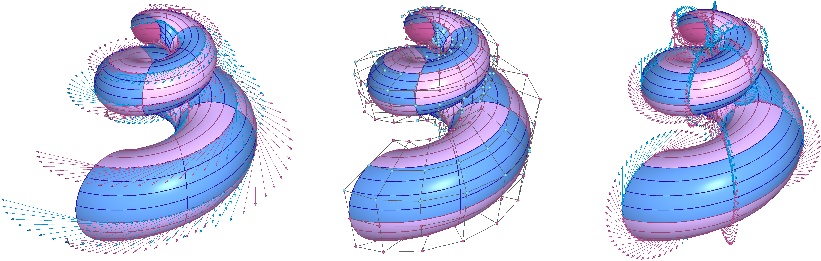
\includegraphics[width =\textwidth]{images/isoparametric_lines_snail.pdf}
		\end{flushright}
		\LinkColor{Defining and using specialized EC spaces  $\bullet$ Differentiating and rendering ordinary and normalized B-basis functions $\bullet$  Creating, manipulating and rendering B-curves and B-surfaces $\bullet$ Generating B-representations of ordinary integral curves and surfaces}
	}
\end{savequote}

\chapter{Usage examples}\label{ch:Usage_examples}

\section{Defining and using specialized EC spaces}\label{sec:Defining_and_using specialized_EC_spaces}

Deriving from the base class \CBlue{ECSpace}, Listings \mref{src:SpecializedECSpaces.h} and \mref{src:SpecializedECSpaces.cpp} define and implement several classes that represent the following polynomial, trigonometric, hyperbolic, algebraic-trigonometric and two algebraic-exponen\-tial-trigonometric EC spaces
\begin{align}
\mathbb{P}_n^{\alpha,\beta}=&~\left\langle\left\{1,u,\ldots,u^n:u\in\left[\alpha,\beta\right]\right\}\right\rangle,
~\dim \mathbb{P}_n^{\alpha,\beta} = n+1,~-\infty < \alpha < \beta < +\infty,
\label{eq:pure_polynomial}
\\
\mathbb{T}_{2n}^{\alpha,\beta}=&~\left\langle\left\{1,\cos\left(u\right),\sin\left(u\right),\ldots,\cos\left(nu\right),\sin\left(nu\right):u\in\left[\alpha,\beta\right]\right\}\right\rangle,
\label{eq:pure_trigonometric}
\\
&~\dim \mathbb{T}_n^{\alpha,\beta} = 2n+1,
~\beta - \alpha \in \left(0,\pi\right),
\nonumber
\\
\mathbb{H}_{2n}^{\alpha,\beta}=&~\left\langle\left\{1,e^u,e^{-u},\ldots,e^{nu},e^{-nu}:u\in\left[\alpha,\beta\right]\right\}\right\rangle,
\label{eq:pure_hyperbolic}
\\
\nonumber
&~\dim \mathbb{H}_n^{\alpha,\beta} = 2n+1,~0 < \beta-\alpha < +\infty, 
\\
\mathbb{AT}_{n\left(n+2\right)}^{\alpha,\beta} =&~
\left\langle
\left\{
1,u,\ldots,u^n,
\left\{
u^r \cos\left(ku\right),
u^r \sin\left(ku\right)
\right\}_{r=0,\,k=1}^{n-k,\,n}:
u \in \left[\alpha,\beta\right]
\right\}
\right\rangle,
\label{eq:algebraic_trigonometric}
\\
&
~\dim \mathbb{AT}_{n\left(n+2\right)}^{\alpha,\beta} = \left(n+1\right)^2,
\nonumber
\\
\mathbb{AET}_{n\left(2n+3\right)}^{\alpha,\beta}
=&~
\left\langle
\left\{
\left\{u^r\right\}_{r=0}^n,
\left\{
u^r e^{ku}\cos\left(ku\right),
u^r e^{ku}\sin\left(ku\right)
\right\}_{r=0,\,k=1}^{n-k,\,n},
\right.
\right.
\label{eq:algebraic-exponential-trigonometric}
\\
&
~~~~\,
\left.
\left.
\left\{
u^r e^{-ku}\cos\left(ku\right),
u^r e^{-ku}\sin\left(ku\right)
\right\}_{r=0,\,k=1}^{n-k,\,n}:
u \in \left[\alpha,\beta\right]
\right\}
\right\rangle,
\nonumber
\\
&
~\dim \mathbb{AT}_{n\left(2n+3\right)}^{\alpha,\beta} = 2n^2+3n+1,
\nonumber
\end{align}
and
\begin{align}
\mathbb{M}_{n+4,a,b}^{\alpha,\beta}=&~
\left\langle
\left\{1,u,\ldots,u^n,
\cosh\left(au\right)\cos\left(bu\right),\cosh\left(au\right)\sin\left(bu\right),\right.\right.
\label{eq:Mazure_vector_space}
\\
&
\left.\left.\sinh\left(au\right)\cos\left(bu\right),\sinh\left(au\right)\sin\left(bu\right)
:
u \in \left[\alpha,\beta\right]
\right\}
\right\rangle,
~
n \geq 0,~a,b>0,
\\
&
~
\dim\mathbb{M}_{n+4,a,b}^{\alpha,\beta}=n+5,
\nonumber{}
\end{align}
respectively.
\begin{remark}It is known that:
    \begin{itemize}
        \item
        the normalized B-basis of $\mathbb{P}_{n}^{\alpha,\beta}$ is formed by the Bernstein polynomials \citep{Carnicer1993} of degree $n$ defined over any non-empty compact interval $\left[\alpha,\beta\right]\subset \mathbb{R}$;
        
        \item
        the unique normalized B-basis of $\mathbb{T}_{2n}^{\alpha,\beta}$ exists whenever $\beta-\alpha \in \left(0,\pi\right)$ and it was constructed in closed form in \citep{Sanchez1998};
        
        \item
        the explicit form of the unique normalized B-basis of the EC space $\mathbb{H}_{2n}^{\alpha,\beta}$ was derived in \citep{ShenWang2005} and, theoretically, the interval length $\beta-\alpha$ can be any positive number (concerning numerical instabilities, the only limitation lies in the usage of potentially too big exponentials);
        
        \item
        for arbitrary values of the order $n \geq 2$, the critical lengths $\ell^{\prime}\left(\mathbb{AT}_{n\left(n+2\right)}^{\alpha,\beta}\right)$ and $ \ell^{\prime}\left(\mathbb{AET}_{n\left(2n+3\right)}^{\alpha,\beta}\right)$ for design and the explicit forms of the unique normalized B-bases of the spaces $\mathbb{AT}_{n\left(n+2\right)}^{\alpha,\beta}$ and  $\mathbb{AET}_{n\left(2n+3\right)}^{\alpha,\beta}$, respectively, were not studied in the literature;  however, normalized B-bases of some special subspaces of these parent spaces were investigated, e.g.,\ in \citep{MainarPena2004,CarnicerMainarPena2004,CarnicerMainarPena2007, MainarPena2010, CarnicerMainarPena2014} and references therein;
    
        \item
        the mixed algebraic-hyperbolic-trigonometric EC space $\mathbb{M}_{n+4,a,b}^{\alpha,\beta}$ was investigated in \citep{BrilleaudMazure2012}, where, for $n=0$, it was shown that $\ell^{\prime}\left(\mathbb{M}_{4,a,b}^{\alpha,\beta}\right)$ coincides with the only solution of the equation $b\tanh\left(au\right)=a \tan\left(bu\right)$, where $u \in \left(\frac{\pi}{b},\frac{3\pi}{2b}\right)$, i.e., in general, the critical length for design is not necessarily a free parameter with respect to the parameters resulting from the differential equation (\ref{eq:differential_equation}); for example, in case of parameters $n=0$, $a=1$ and $b = 0.2$ one obtains that $\ell^{\prime}\left(\mathbb{M}_{4,1,0.2}^{\alpha,\beta}\right)\approx 16.694941067922716$, i.e., the space $\mathbb{M}_{4,1,0.2}^{\alpha,\beta}$ possesses a unique normalized B-basis provided that $\beta - \alpha \in \left(0,16.694941067922716\right)$; moreover, $\ell^{\prime}\left(\mathbb{M}_{n+4,a,b}^{\alpha,\beta}\right)\geq \ell^{\prime}\left(\mathbb{M}_{4,a,b}^{\alpha,\beta}\right),~\forall n\geq 1$, $\forall a,b>0$.
        
    \end{itemize}
    
\end{remark}
Following the provided examples, the user can also implement other special EC spaces that comprise the constant functions and can be identified with the solution spaces of constant-coefficient homogeneous linear differential equations of type (\mref{eq:differential_equation}). Note that in Listing \mref{src:SpecializedECSpaces.cpp}, apart from some natural exception handling, the constructors of the aforementioned derived classes only specify the factorization of the characteristic polynomial (\mref{eq:characteristic_polynomial}) of the differential equation (\mref{eq:differential_equation}), and by doing this both well-known and new types of normalized B-bases can easily be constructed (on intervals having appropriate lengths), by writing only a few lines of code.
 
\ccodeNUV{1}{listings/Examples/01/SpecializedECSpaces.h}{src:SpecializedECSpaces.h}{Specialized EC spaces (\textbf{SpecializedECSpaces.h})}{1}

\ccodeNUV{1}{listings/Examples/01/SpecializedECSpaces.cpp}{src:SpecializedECSpaces.cpp}{Specialized EC spaces (\textbf{SpecializedECSpaces.cpp})}{1}

\section{Using our shader programs}\label{sec:Using_our_shader_programs}

Classes \CBlue{GenericCurve3}, \CBlue{TriangleMesh3}, \CBlue{BCurve3}:\ \CRed{public} \CBlue{LinearCombination3} and \CBlue{BSurface3}:\ \CRed{public} \CBlue{TensorProductSurface3} provide several rendering methods. Each of them have two variants, the first of these overloaded member functions relies on instances of our class \CBlue{ShaderProgram}, while the second one assumes that users handle their shader programs in a different way by providing at the same time attribute (like position, color, normal and texture coordinate) locations of proper types as input parameters for this second variant of our rendering methods. The latter variants will return a false value whenever one of the followings happens: the users did not activate their custom shader programs; the given attribute locations cannot be found in the list of active attribute locations, or they exist but are associated with attributes that have incorrect types (positions, colors, normals and texture coordinate attribute variables have to be of types \CRed{vec3}, \CRed{vec4}, \CRed{vec3} and \CRed{vec4}, respectively); the rendering mode or other input parameters are invalid. For more details consider the lines \mref{src:GenericCurve3:renderDerivatives:start}--\mref{src:GenericCurve3:renderDerivatives:end}, \mref{src:TrinagleMesh3:render:start}--\mref{src:TrinagleMesh3:render:end},  \mref{src:LinearCombination3:renderData:start}--\mref{src:LinearCombination3:renderData:end} and \mref{src:TensorProductSurface3:render:start}--\mref{src:TensorProductSurface3:render:end} of Listings \mref{src:GenericCurves3.h}, \mref{src:TriangleMeshes3.h},  \mref{src:LinearCombinations3.h} and \mref{src:TensorProductSurfaces3.h}, respectively.

For convenience we have also provided shader programs for simple (flat) color shading, for two-sided per pixel lighting that is able to handle user-defined directional, point and spotlights with uniform front and back materials, and another one for reflection lines that are combined with two-sided per pixel lighting. All figures of this user manual were rendered by using these shader programs. If these would not be sufficient, more experienced users are invited to implement and use their custom shader programs and to append the provided function library with new special effects like in an open source project.

\subsection{Simple (flat) color vertex and fragment shaders}

Vertex buffer objects that store curve points, first and higher order derivatives, control polygons or nets do not provide coordinates for normal vectors. Therefore, in order to render these geometric objects, we advise to use the simple (flat) color vertex and fragment shaders that are presented in Listings \mref{src:color.vert} and \mref{src:color.frag}, respectively. 

\ccode{1}{listings/Examples/00/Shaders/color.vert}{src:color.vert}{Simple color vertex shader}{1}

The uniform variable PVM of type \CRed{mat4} declared in line \mref{src:color.vert:PVM} of Listing \mref{src:color.vert} denotes the product of the (either perspective or orthogonal) projection, of the view (i.e., camera) and of the model transformation (i.e., rotation, translation and scaling) matrices that were provided in Listing \mref{src:SpecialGLTransformations.h} as special OpenGL transformations. At the CPU-side, multiplications of these special transformation matrices can be performed by using the arithmetical multiplication operators inherited from their common generic base class \CBlue{GLTransformation} that is defined and implemented in Listings \mref{src:GenericGLTransformations.h} and \mref{src:GenericGLTransformations.cpp}, respectively. The constant address of the memory-continuous constant \CRed{float} array that stores the obtained $4\times 4$ column-major ordered transformation matrix can be queried by the method \CBlue{GLTransformation}::address() that is declared in line \mref{src:GLTransformation:address:declaration} of Listing \mref{src:GenericGLTransformations.h}. By passing this pointer as the fourth input parameter to the method \CPurple{GLboolean} \CBlue{ShaderProgram}::setUniformMatrix4fv(\CRed{const std}::\CRed{string} \&name, \CPurple{GLsizei} count, \CPurple{GLboolean} transpose, \CRed{const} \CPurple{GLfloat} *values) declared in line \mref{src:ShaderProgram:setUniformMatrix4fv:declaration} of Listing \mref{src:ShaderPrograms.h}, one can initialize the uniform matrix variable PVM.

Note that, our \CBlue{ShaderProgram} objects assume by default that the name of the position attribute is ``position", while its type is \CRed{vec3}. If required, this attribute name can be changed by using the method \CPurple{GLvoid} \CBlue{ShaderProgram}::setPositionAttributeName(\CRed{const std}::\CRed{string} \&name) declared in line \mref{src:ShaderProgram:setPositionAttributeName:declaration} of Listing \mref{src:ShaderPrograms.h}.

\ccode{1}{listings/Examples/00/Shaders/color.frag}{src:color.frag}{Simple color fragment shader}{1}

The uniform variable color of type \CRed{vec4} declared in line \mref{src:color.frag:color} of Listing \mref{src:color.frag} can be initialized by using one of the methods 
\CPurple{GLboolean} \CBlue{ShaderProgram}::setUniformValue4f(\CDRRed{const std}::\CDRRed{string} \&name, \CPurple{GLfloat} value\_0, \CPurple{GLfloat} value\_1,
\CPurple{GLfloat} value\_2, \CPurple{GLfloat} value\_3)
,
\CPurple{GLboolean} \CBlue{ShaderProgram}::\allowbreak{}set\-Uniform\-Value4fv(\CDRRed{const std}::\CDRRed{string} \&name, \CPurple{GLsizei} count, \CRed{const} \CPurple{GLfloat} *values)
or
\CPurple{GLboolean} \CBlue{ShaderProgram}::setUniformColor(\CDRRed{const std}::\CDRRed{string} \&name, \CDRRed{const} \CBlue{Color4} \&color) that are declared in lines \mref{src:ShaderProgram:setUniformValue4f:declaration}, \mref{src:ShaderProgram:setUniformValue4fv:declaration} and \mref{src:ShaderProgram:setUniformColor:declaration}, respectively, of Listing \mref{src:ShaderPrograms.h}.

In our examples, we will frequently use some predefined colors that are specified in lines \mref{src:Color4:colors:start}--\mref{src:Color4:colors:end} of Listing \mref{src:Colors4.h}. Moreover, in order to express some value dependent color variation, we will also use the color generation function \CBlue{Color4 coldToHotColormap}(\CPurple{GLfloat} value, \CPurple{GLfloat} min\_value, \CPurple{GLfloat} max\_value) that is declared and implemented in the lines \mref{src:Utilities:coldToHotColormap:declaration} and \mref{src:Utilities:coldToHotColormap:start}--\mref{src:Utilities:coldToHotColormap:end} of Listings \mref{src:Utilities.h} and \mref{src:Utilities.cpp}, respectively.

Examples for the usage of simple color shaders can be found in Listing pairs \mref{src:GLWidgetTestingShaderPrograms.h}--\mref{src:GLWidgetTestingShaderPrograms.cpp}, \mref{src:GLWidgetDifferentiatingAndRenderingBasisFunctions.h}--\mref{src:GLWidgetDifferentiatingAndRenderingBasisFunctions.cpp}, \mref{src:GLWidgetDefineEvaluateDifferentiateManipulateRenderBCurves.h}--\mref{src:GLWidgetDefineEvaluateDifferentiateManipulateRenderBCurves.cpp}, \mref{src:GLWidget_exmp_03.h}--\mref{src:GLWidget_exmp_03.cpp}, \mref{src:GLWidgetTestingBSurfaceOperations.h}--\mref{src:GLWidgetTestingBSurfaceOperations.cpp} and \mref{src:GLWidgetSnail.h}--\mref{src:GLWidgetSnail.cpp}.

\subsection{Two-sided per pixel lighting}

In order to provide two-sided per pixel lighting, one can use the vertex and fragment shaders presented in Listings \mref{src:two_sided_lighting.vert} and \mref{src:two_sided_lighting.frag}, respectively. With some modifications, these shaders are based on \citep{RostLiceaKane2006}. Examples for their usage can be found in Listing pairs \mref{src:GLWidgetTestingShaderPrograms.h}--\mref{src:GLWidgetTestingShaderPrograms.cpp},  \mref{src:GLWidgetTestingBSurfaceOperations.h}--\mref{src:GLWidgetTestingBSurfaceOperations.cpp} and \mref{src:GLWidgetSnail.h}--\mref{src:GLWidgetSnail.cpp}.

\ccodeNUV{1}{listings/Examples/00/Shaders/two_sided_lighting.vert}{src:two_sided_lighting.vert}{Vertex shader of the two-sided per pixel lighting and of reflection lines}{1}

\ccodeNUV{1}{listings/Examples/00/Shaders/two_sided_lighting.frag}{src:two_sided_lighting.frag}{Fragment shader of the two-sided per pixel lighting}{1}

\subsection{Reflection lines combined with two-sided per pixel lighting}

The vertex shader of the reflection lines coincides with that of the two-sided per pixel lighting presented in Listing \mref{src:two_sided_lighting.vert}. By modifying a free fragment shader created by Ga\"el Guennebaud for the powerful mesh processing tool \href{http://meshlab.sourceforge.net/}{MeshLab}, the fragment shader of the reflection lines is implemented in Listing \mref{src:reflection_lines.frag} that -- compared with the fragment shader of the two-sided per pixel lighting listed in Listing \mref{src:two_sided_lighting.frag} -- introduces some new constants and uniform variables, and at the same time also appends the code with reflection line (or zebra stripe) generation. (The newly appended code snippets are included between consecutive pairs of red and blue horizontal lines.)

\ccodeNUV{1}{listings/Examples/00/Shaders/reflection_lines+.frag}{src:reflection_lines.frag}{Fragment shader of reflection lines}{1}

Examples for the usage of the reflection lines generating shader can be found in Listing pairs \mref{src:GLWidgetTestingShaderPrograms.h}--\mref{src:GLWidgetTestingShaderPrograms.cpp},  \mref{src:GLWidgetTestingBSurfaceOperations.h}--\mref{src:GLWidgetTestingBSurfaceOperations.cpp} and \mref{src:GLWidgetSnail.h}--\mref{src:GLWidgetSnail.cpp}.

\ccode{1}{listings/Examples/00/Shaders/GLWidgetTestingShaderPrograms.h}{src:GLWidgetTestingShaderPrograms.h}{Using the provided shader programs}{1}

\ccode{1}{listings/Examples/00/Shaders/GLWidgetTestingShaderPrograms.cpp}{src:GLWidgetTestingShaderPrograms.cpp}{Using the provided shader programs}{1}


\section{Differentiating and rendering basis functions}\label{sec:Differentiating_and_rendering_basis_functions}

Once an EC space object is created, one can differentiate and render both its ordinary basis and normalized B-basis functions. Listings \mref{src:GLWidgetDifferentiatingAndRenderingBasisFunctions.h} and \mref{src:GLWidgetDifferentiatingAndRenderingBasisFunctions.cpp}  declare and define data structures for the evaluation and rendering of the unique normalized B-bases of the EC spaces $\mathbb{P}_{10}^{0,1}$, $\mathbb{T}_{10}^{0,\frac{\pi}{2}}$, $\mathbb{H}_{14}^{0,\pi}$, $\mathbb{AT}_{24}^{0,2\pi}$, $\mathbb{AET}_{27}^{-5\pi/4,\,5\pi/4}$ and $\mathbb{M}_{n+4,1,0.2}^{0,\beta}$ that are of types (\mref{eq:pure_polynomial}), (\mref{eq:pure_trigonometric}), (\mref{eq:pure_hyperbolic}), (\mref{eq:algebraic_trigonometric}), (\mref{eq:algebraic-exponential-trigonometric}) and (\mref{eq:Mazure_vector_space}), respectively, where $\beta = 16.694941067922716$.

%\ccodeNUV{1}{src/Examples/01/GLWidget+.h}{src:GLWidget_exmp_01.h}{Differentiating and rendering basis functions (\textbf{Renderable.h})}{1}

\newpage{}

\ccodeNUV{1}{listings/Examples/01/GLWidgetDifferentiatingAndRenderingBasisFunctions.h}{src:GLWidgetDifferentiatingAndRenderingBasisFunctions.h}{Differentiating and rendering basis functions (\textbf{YourGLWidget.h})}{1}

\ccodeNUV{1}{listings/Examples/01/GLWidgetDifferentiatingAndRenderingBasisFunctions.cpp}{src:GLWidgetDifferentiatingAndRenderingBasisFunctions.cpp}{Differentiating and rendering basis functions (\textbf{YourGLWidget.cpp})}{1}

%\ccodeNUV{1}{src/Examples/01/GLWidget+.cpp}{src:GLWidget_exmp_01.cpp}{Differentiating and rendering basis functions (\textbf{Renderable.cpp})}

\begin{figure}[!htb]
    \centering
    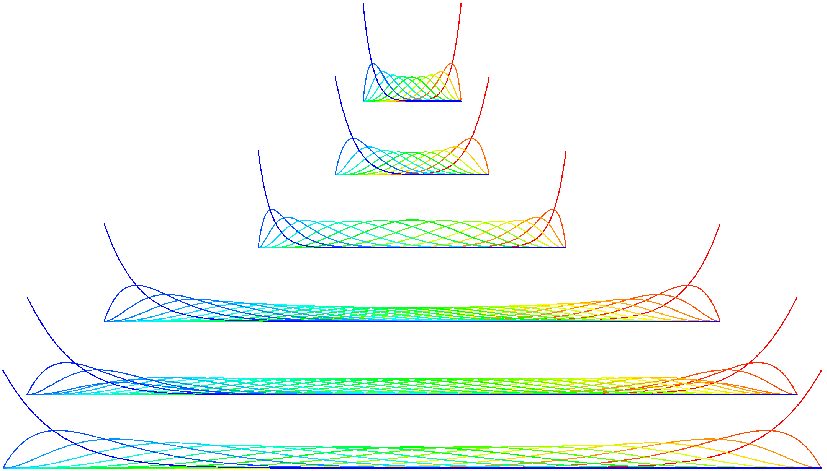
\includegraphics[]{images/differentiation_and_rendering_of_B_bases+.pdf}
    \caption{From top to bottom: evaluation and rendering of the unique normalized B-bases of the EC spaces $\mathbb{P}_{10}^{0,1}$, $\mathbb{T}_{10}^{0,\frac{\pi}{2}}$, $\mathbb{H}_{14}^{0,\pi}$, $\mathbb{AT}_{24}^{0,2\pi}$, $\mathbb{AET}_{27}^{-5\pi/4,5\pi/4}$ and $\mathbb{M}_{14,1,0.2}^{0,\beta}$ that are of types (\mref{eq:pure_polynomial}), (\mref{eq:pure_trigonometric}), (\mref{eq:pure_hyperbolic}), (\mref{eq:algebraic_trigonometric}), (\mref{eq:algebraic-exponential-trigonometric}) and (\mref{eq:Mazure_vector_space}), respectively, where $\beta = \frac{1}{2}\cdot 16.694941067922716 = 8.347470533961358$. (The figure was generated by the source codes listed in Listings \mref{src:GLWidgetDifferentiatingAndRenderingBasisFunctions.h} and \mref{src:GLWidgetDifferentiatingAndRenderingBasisFunctions.cpp}.)}
    \label{fig:differentiation_and_rendering_of_B_bases}
\end{figure}

\section{Defining and using specialized B-curves}\label{sec:Defining_and_using_specialized_EC_B-curves}

The next two subsections provide examples for the description and manipulation of B-curves defined in different types of EC spaces.

\subsection{B-curve generation, order elevation and subdivision}\label{subsec:B-curve_generation_order_elevation_and_subdivision}

EC space objects can also be used to define, evaluate, differentiate, manipulate and render B-curves of type (\mref{eq:B_curve}) and to perform order elevations and subdivisions on them as it is illustrated in Listings \mref{src:GLWidgetDefineEvaluateDifferentiateManipulateRenderBCurves.h} and \mref{src:GLWidgetDefineEvaluateDifferentiateManipulateRenderBCurves.cpp} in case of five different EC spaces.

\ccodeNUV{1}{listings/Examples/02/GLWidgetDefineEvaluateDifferentiateManipulateRenderBCurves.h}{src:GLWidgetDefineEvaluateDifferentiateManipulateRenderBCurves.h}{Defining, rendering, order elevating and subdividing B-curves (\textbf{YourGLWidget.h})}{1}

\ccodeNUV{1}{listings/Examples/02/GLWidgetDefineEvaluateDifferentiateManipulateRenderBCurves.cpp}{src:GLWidgetDefineEvaluateDifferentiateManipulateRenderBCurves.cpp}{Defining, rendering, order elevating and subdividing B-curves (\textbf{YourGLWidget.cpp})}{1}

\begin{figure}[!htb]
	\centering
	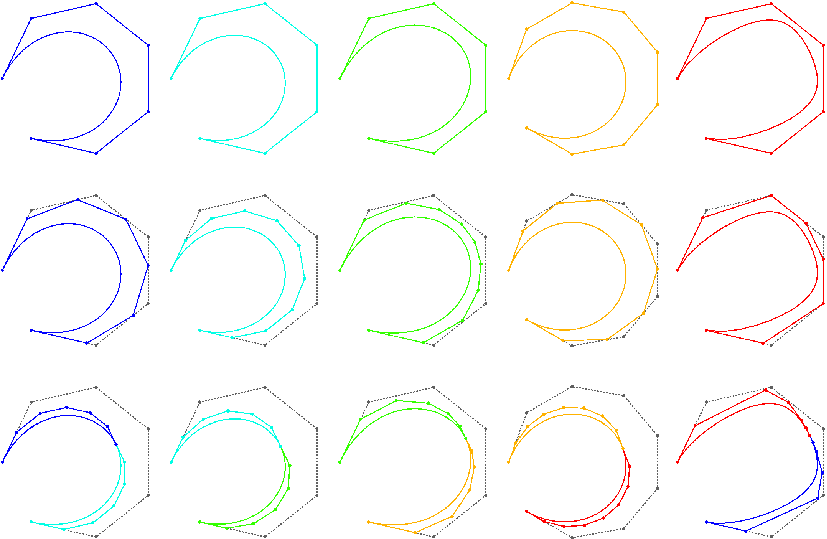
\includegraphics[]{images/B-curve_operations+.pdf}
	\caption{From left to right: the columns illustrate the order elevation and subdivision of different B-curves in EC spaces $\mathbb{P}_{6}^{0,1}$, $\mathbb{T}_{6}^{0,\frac{\pi}{2}}$, $\mathbb{H}_{6}^{0,\pi}$, $\mathbb{AT}_{8}^{0,\frac{4\pi}{3}}$ and $\mathbb{M}_{6,1,0.2}^{0,16.694941067922716}$ that are of types (\mref{eq:pure_polynomial}), (\mref{eq:pure_trigonometric}), (\mref{eq:pure_hyperbolic}), (\mref{eq:algebraic_trigonometric}) and (\mref{eq:Mazure_vector_space}), respectively. (The figure was generated by the source codes listed in Listings \mref{src:GLWidgetDefineEvaluateDifferentiateManipulateRenderBCurves.h} and \mref{src:GLWidgetDefineEvaluateDifferentiateManipulateRenderBCurves.cpp}.)}
	\label{fig:B-curve_operations}
\end{figure}

\subsection{B-representation of ordinary integral curves}\label{subsec:B_representation_of_ordinary_integral_curves}

B-curves can also be used to provide control point based exact descriptions (or B-representations) for ordinary integral curves of type (\mref{eq:ordinary_integral_curve}) as it is illustrated in Listings \mref{src:GLWidget_exmp_03.h} and \mref{src:GLWidget_exmp_03.cpp}, which at first define the EC space
\begin{align*}
\mathbb{S}_4^{0,\beta}
=&~
\left\langle
\left\{
\varphi_{4,0}\left(u\right) \equiv 1,
\varphi_{4,1}\left(u\right)=e^{-\omega u} \cos\left(u\right),
\varphi_{4,2}\left(u\right)=e^{-\omega u} \sin\left(u\right),
\right.
\right.
\\
&~~~\,
\left.
\left.
\varphi_{4,3}\left(u\right)=e^{\omega u} \cos\left(u\right),
\varphi_{4,4}\left(u\right)=e^{\omega u} \sin\left(u\right):
u \in \left[0,\beta\right]
\right\}
\right\rangle,~\beta \in \left(0,\pi\right]
\end{align*}
where $\omega = \frac{1}{3\pi}$, then they also generate B-curves for the B-representations of the logarithmic spiral arcs 
\begin{align}
\mathbf{c}_k\left(u\right) &=
\left[
\begin{array}{c}
e^{\omega \left(u+k\beta\right)} \cos\left(u+k\beta\right)\\
e^{\omega \left(u+k\beta\right)} \sin\left(u+k\beta\right)
\end{array}
\right]
\nonumber
\\
&=
e^{k\omega\beta}
\left[
\begin{array}{c}
\cos\left(k\beta\right)
\\
\sin\left(k\beta\right)
\end{array}
\right]
\varphi_{4,3}\left(u\right)
+
e^{k\omega\beta}
\left[
\begin{array}{r}
-\sin\left(k\beta\right)\\
\cos\left(k\beta\right)
\end{array}
\right]
\varphi_{4,4}\left(u\right), ~ u \in \left[0,\beta\right],~k=0,\ldots,6.
\label{eq:logarithmic_spiral}
\end{align}

\newpage{}

\ccodeNUV{1}{listings/Examples/03/GLWidget.h}{src:GLWidget_exmp_03.h}{B-representations of ordinary integral curves (\textbf{YourGLWidget.h})}{1}

\ccodeNUV{1}{listings/Examples/03/GLWidget.cpp}{src:GLWidget_exmp_03.cpp}{B-representations of ordinary integral curves (\textbf{YourGLWidget.cpp})}{1}

\begin{figure}[!htb]
	\centering
	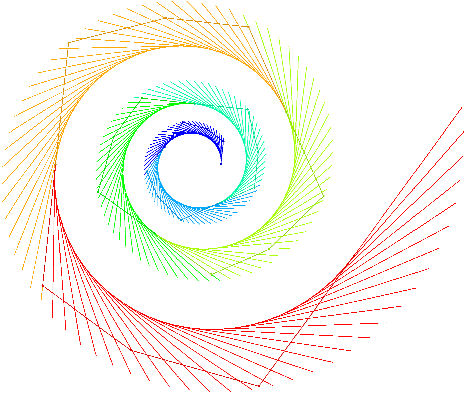
\includegraphics[]{images/logarithmic_spiral.pdf}
	\caption{Control point based exact description (or B-representation) of different arcs of a logarithmic spiral. (The figure was generated by the source codes given in Listings \mref{src:GLWidget_exmp_03.h} and \mref{src:GLWidget_exmp_03.cpp}.)}
	\label{fig:logarithmic_spiral}
\end{figure}

\section{Defining and using specialized B-surfaces}\label{sec:Defining_and_using_specialized_EC_B-surfaces}

The next two subsections provide examples for the description and manipulation of B-surfaces defined in different types of EC spaces.

\subsection{B-surface generation, order elevation and subdivision}\label{subsec:B-surface_generation_order_elevation_and_subdivision}

Listings \mref{src:GLWidgetTestingBSurfaceOperations.h} and \mref{src:GLWidgetTestingBSurfaceOperations.cpp} provide examples for the generation, evaluation, order elevation, subdivision and rendering of B-surfaces.

\newpage{}

\ccode{1}{listings/Examples/04/GLWidgetTestingBSurfaceOperations.h}{src:GLWidgetTestingBSurfaceOperations.h}{Defining, rendering, order elevating and subdividing B-surfaces (\textbf{YourGLWidget.h})}{1}

\ccode{1}{listings/Examples/04/GLWidgetTestingBSurfaceOperations.cpp}{src:GLWidgetTestingBSurfaceOperations.cpp}{Defining, rendering, order elevating and subdividing B-surfaces (\textbf{YourGLWidget.cpp})}{1}

\begin{figure}[!htb]
    \centering
    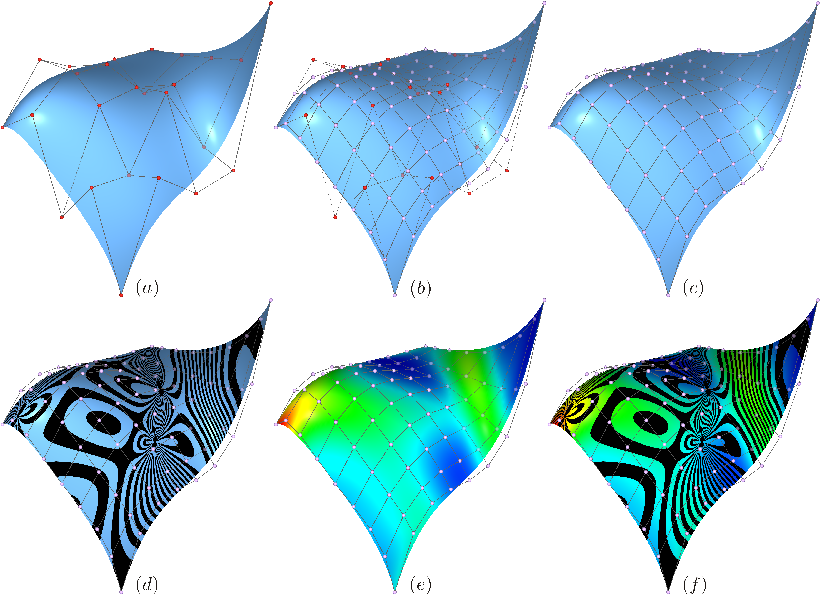
\includegraphics[]{images/B_surface_order_elevation.pdf}
    \caption{(\textit{a}) Randomly generated initial B-surface, rendered with a simple color material together with its control net. (\textit{b}) Order elevation of the initial B-surface, rendered with a simple color material together with its initial and order elevated control nets. (\textit{c}) The order elevated B-surface, rendered with a simple color material together with its control net. (\textit{d}) The order elevated B-surface, rendered with a simple color material together with its control net and reflection lines. (\textit{d}) The order elevated B-surface, rendered with the logarithmic umbilic deviation color scheme together with its control net. (\textit{e}) The order elevated B-surface, rendered with the translated logarithmic scale of the umbilic deviation color scheme together with its control net and reflection lines. (The figure was generated by the source codes given in Listings \mref{src:GLWidgetTestingBSurfaceOperations.h} and \mref{src:GLWidgetTestingBSurfaceOperations.cpp}.)}
    \label{fig:B_surface_order_elevation}
\end{figure}

\begin{figure}[!htb]
    \centering
    \includegraphics[]{images/color_schemes.pdf}
    \caption{The figure was generated by the source codes given in Listings \mref{src:GLWidgetTestingBSurfaceOperations.h} and \mref{src:GLWidgetTestingBSurfaceOperations.cpp}. (\textit{a})--($\ell$) The color schemes correspond to the point-wise variations of the $x$-, $y$- and $z$-coordinates, of the length of the normal vectors, of the Gaussian- and mean curvatures, of the Willmore energy and its translated logarithmic counterpart, of the umbilic deviation and its translated logarithmic scale, of the total curvature and its translated logarithmic variant, respectively. (In each case the applied color map behaves like a temperature variation that ranges from the cold dark blue to the hot red, by passing through the colors cyan, green, yellow and orange such that the minimal and maximal values of a fixed energy type correspond to the extremal colors dark blue and red, respectively. For more details, see the lines  \mref{src:Utilities:coldToHotColormap:rainbow}--\mref{src:Utilities:coldToHotColormap:end} and \mref{src:TensorProductSurface3.h:ImageColorScheme:start}--\mref{src:TensorProductSurface3.h:ImageColorScheme:end} of Listings \mref{src:Utilities.cpp} and \mref{src:TensorProductSurfaces3.h}, respectively.)}
    \label{fig:color_schemes}
\end{figure}

\begin{figure}[!htb]
    \centering
    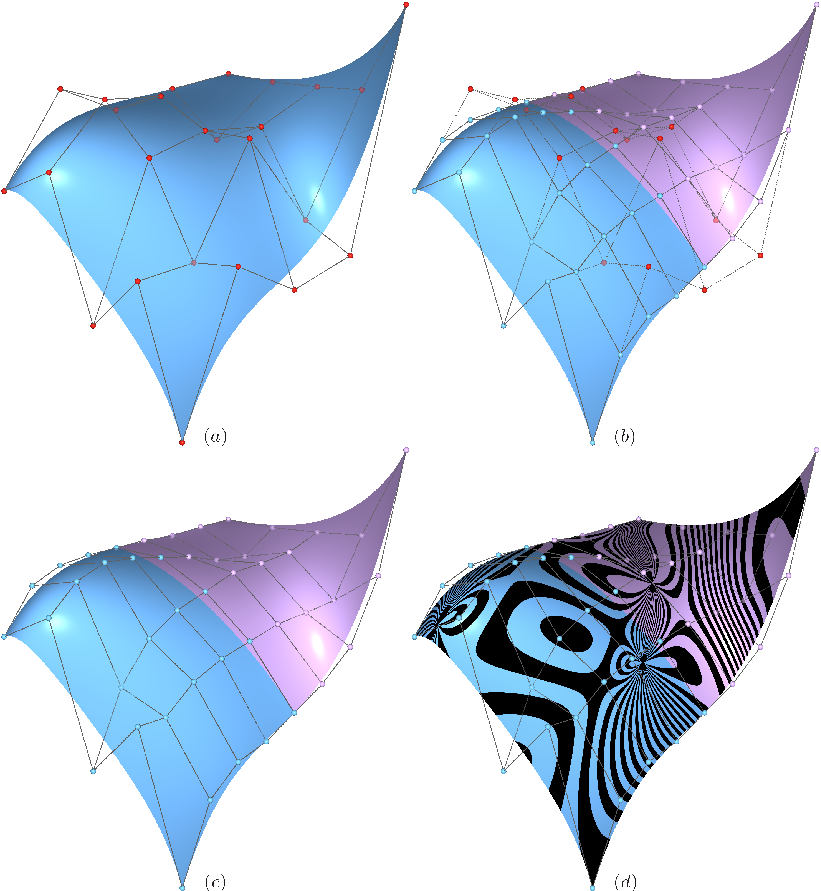
\includegraphics[]{images/B_surface_subdivision_u.pdf}
    \caption{(\textit{a}) A randomly generated initial B-surface, rendered with a simple color material together with its control net. (\textit{b}) Subdivision of the given B-surface in direction $u$. The obtained B-patches are rendered with simple color materials together with the control net of the initial B-surface and with their control nets. (\textit{c}) The obtained B-patches are rendered with simple color materials together with their control nets. (\textit{d}) The obtained B-patches are rendered with simple color materials together with their control nets and smooth reflection lines. (The figure was generated by the source codes given in Listings \mref{src:GLWidgetTestingBSurfaceOperations.h} and \mref{src:GLWidgetTestingBSurfaceOperations.cpp}.)}
    \label{fig:B_surface_subdivision_u}
\end{figure}

\begin{figure}[!htb]
    \centering
    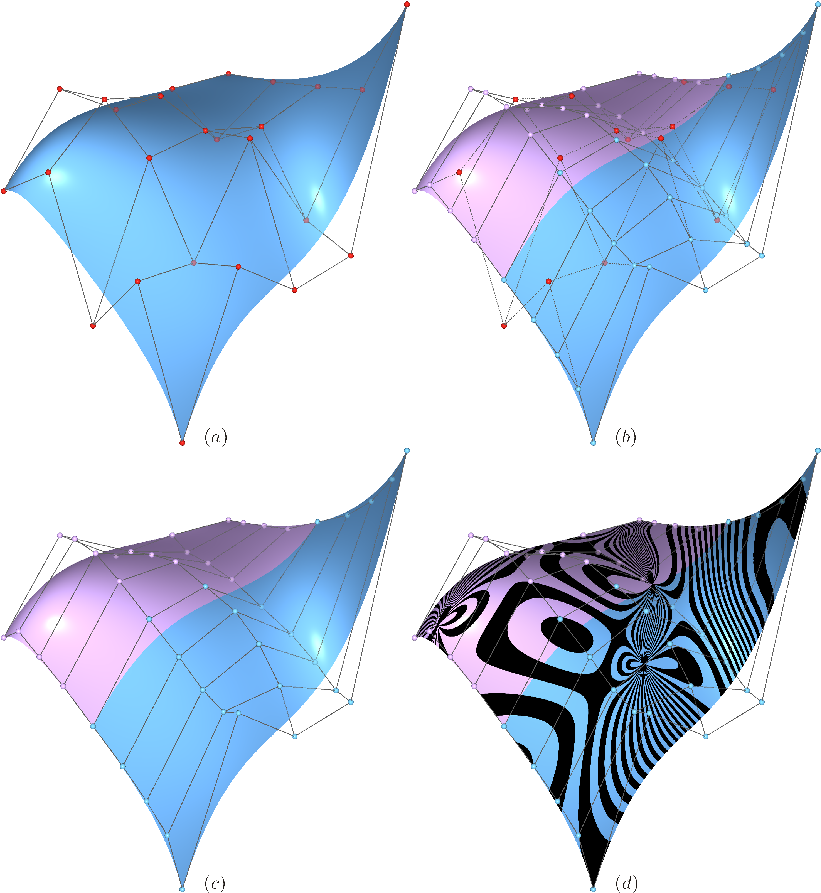
\includegraphics[]{images/B_surface_subdivision_v.pdf}
    \caption{(\textit{a}) A randomly generated initial B-surface, rendered with a simple color material together with its control net. (\textit{b}) Subdivision of the given B-surface in direction $v$. The obtained B-patches are rendered with simple color materials together with the control net of the initial B-surface and with their control nets. (\textit{c}) The obtained B-patches are rendered with simple color materials together with their control nets. (\textit{d}) The obtained B-patches are rendered with simple color materials together with their control nets and smooth reflection lines. (The figure was generated by the source codes given in Listings \mref{src:GLWidgetTestingBSurfaceOperations.h} and \mref{src:GLWidgetTestingBSurfaceOperations.cpp}.)}
    \label{fig:B_surface_subdivision_v}
\end{figure}

\subsection{B-representation of ordinary integral surfaces}\label{subsec:B-representation_of_ordinary_integral_surfaces}

B-surfaces can also be used to provide control point configurations for the exact description (or B-representation) of ordinary integral surfaces of type (\mref{eq:ordinary_integral_surface}) as it is illustrated in Listings \mref{src:GLWidgetSnail.h} and \mref{src:GLWidgetSnail.cpp}. We also show how can one evaluate and render the zeroth and higher order partial derivatives of the isoparametric lines of arbitrary B-surfaces. As we will see, the mentioned listings at first define the mixed exponential-trigonometric and pure trigonometric EC spaces
\begin{align*}
\mathbb{ET}_6^{\alpha_0^k,\beta_0^k}
=&~
\left\langle
\left\{
\varphi_{6,0}\left(u\right) \equiv 1,
\varphi_{6,1}\left(u\right)=\cos\left(u\right),
\varphi_{6,2}\left(u\right)=\sin\left(u\right),
\varphi_{6,3}\left(u\right)=e^{\omega_0 u},
\varphi_{6,4}\left(u\right)=e^{\omega_1 u},
\right.
\right.
\\
&~~~\,
\left.
\left.
\varphi_{6,5}\left(u\right)=e^{\omega_0 u} \cos\left(u\right),
\varphi_{6,6}\left(u\right)=e^{\omega_0 u} \sin\left(u\right):
u \in \left[\alpha_0^k,\beta_0^k\right]
\right\}
\right\rangle,~k=0,1,\ldots,4
\end{align*}
and
\[
\mathbb{T}_2^{\alpha_1^{\ell}, \beta_1^{\ell}} =
\left\langle
\left\{
\varphi_{2,0}\left(v\right) \equiv 1, 
\varphi_{2,1}\left(v\right)=\cos\left(v\right),
\varphi_{2,2}\left(v\right)=\sin\left(v\right) :
v \in \left[\alpha_1^{\ell}, \beta_1^{\ell}\right]
\right\}
\right\rangle,~\ell = 0,1,\ldots,\left\lfloor 3\tau \right\rfloor,
\]
respectively, where 
\begin{align*}
\omega_0 &= \frac{1}{6\pi},\\
\omega_1 &= \frac{1}{3\pi},\\
\alpha_0^k &= \frac{7\pi}{2}+\frac{29\pi}{40}\cdot k,~k=0,1,\ldots,4,\\
\beta_0^k  &= \alpha_0^k + \frac{29\pi}{40},~k=0,1,\ldots,4,\\
\alpha_1^{\ell} &= -\frac{\pi}{3\tau}+\frac{2\pi}{\left\lfloor 3\tau\right\rfloor}\cdot\ell,~\ell=0,1,\ldots,\left\lfloor 3\tau\right\rfloor,~\tau \geq 1,\\
\beta_1^{\ell}  &= \alpha_1^{\ell} + \frac{2\pi}{\left\lfloor 3\tau\right \rfloor},~\ell=0,1,\ldots,\left\lfloor 3\tau\right\rfloor,
\end{align*}
then they also generate B-surfaces for the B-representations of the ordinary surface patches 
\begin{align}
\mathbf{s}_{k,\ell}\left(u,v\right) =
\def\arraystretch{1.3}
%\left[\begin{array}{c}s^0\left(u, v\right)\\s^1\left(u, v\right)\\s^2\left(u, v\right)\end{array}\right]
%=
\left[\begin{array}{c}\left(1-e^{\omega_0 u}\right) \cos\left(u\right) \left(\frac{5}{4}+\cos\left(v\right)\right)\\\left(e^{\omega_0 u}-1\right) \sin\left(u\right) \left(\frac{5}{4}+\cos\left(v\right)\right)\\7-e^{\omega_1 u} - \sin\left(v\right) + e^{\omega_0 u} \sin\left(v\right)\end{array}\right],\def\arraystretch{1.0} 
~
\left(u,v\right)\in\left[\alpha_0^k, \beta_0^k\right]\times\left[\alpha_1^{\ell}, \beta_1^{\ell}\right],
\label{eq:snail}
\end{align}
where $k=0,1,\ldots,4$ and $\ell = 0,1,\ldots,\left\lfloor 3\tau\right\rfloor$.

\newpage{}

\ccode{1}{listings/Examples/05/GLWidgetSnail.h}{src:GLWidgetSnail.h}{B-representations of ordinary integral surfaces and their isoparametric lines (\textbf{YourGLWidget.h})}{1}

\ccode{1}{listings/Examples/05/GLWidgetSnail.cpp}{src:GLWidgetSnail.cpp}{B-representations of ordinary integral surfaces and their isoparametric lines (\textbf{YourGLWidget.cpp})}{1}

\begin{figure}[!htb]
    \centering
    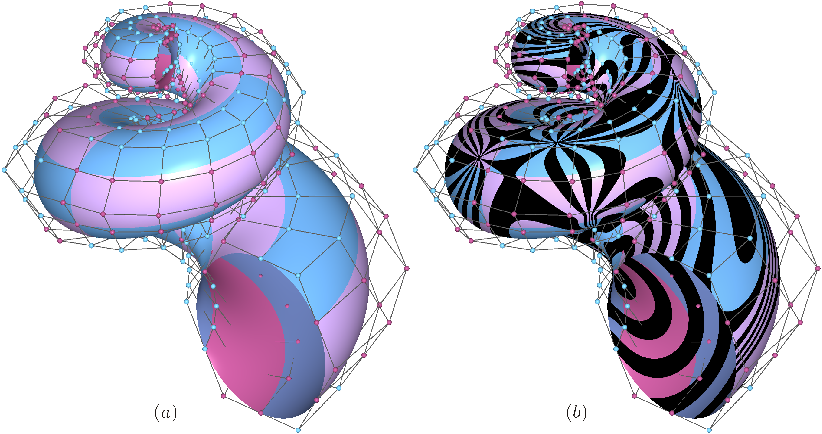
\includegraphics[]{images/control_point_based_exact_description_snail_tau_2.pdf}
    \caption{A possible control point based exact description (or B-representation) of the ordinary exponential-trigonometric integral surface (\mref{eq:snail}) by means of a $5 \times 6$ matrix of B-surface patches. (\textit{a}) Using alternating simple color materials, the obtained B-surface patches are rendered together with their control nets. (\textit{b}) Using alternating simple color materials, the obtained B-surface patches are rendered together with their control nets and smooth reflection lines. (The figure was generated by the source codes given in Listings \mref{src:GLWidgetSnail.h} and \mref{src:GLWidgetSnail.cpp}.)}
    \label{fig:control_point_based_exact_description_snail_tau_2}
\end{figure}

\begin{figure}[!htb]
    \centering
    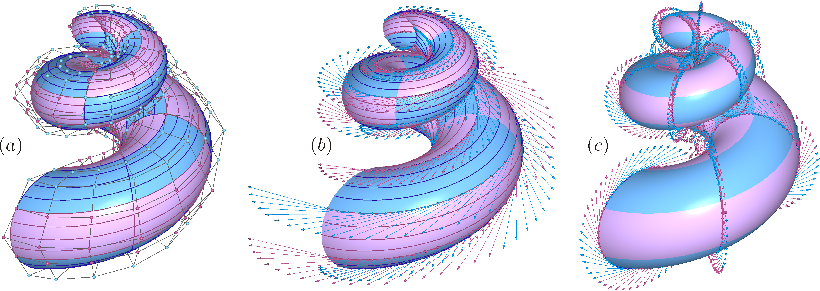
\includegraphics[]{images/isoparametric_lines_snail_user_manual.pdf}
    \caption{Isoparametric lines and their tangent vectors in case of a possible B-representation of the ordinary exponential-trigonometric integral surface (\mref{eq:snail}). Along all $5\times 6 = 30$ B-surface patches we have generated $5$ and $3$ isoparametric lines in directions $u$ and $v$, respectively. The $u$- and $v$-isoparametric lines consist of $20$ and $10$ subdivision points, respectively. (For better visibility, we have rendered the tangent vectors only of some of the isoparametric lines.) (\textit{a}) Surface patches, rendered with alternating simple color materials together with their control nets and isoparametric lines. (\textit{b}) $u$-directional isoparametric lines and their tangent vectors. (\textit{c}) $v$-directional isoparametric lines and their tangent vectors. (The figure was generated by the source codes given in Listings \mref{src:GLWidgetSnail.h} and \mref{src:GLWidgetSnail.cpp}.)}
    \label{fig:isoparametric_lines_user_manual}
\end{figure}

\backmatter

\bibliographystyle{ACM-Reference-Format}
\bibliography{refs}

\end{document}
